\documentclass[10pt,a4paper]{elsarticle}
\usepackage[utf8]{inputenc}
\usepackage[T1]{fontenc}
\usepackage{amsmath}
\usepackage{amsfonts}
\usepackage{amssymb}
\usepackage{graphicx}
\usepackage{mathtools,amssymb}
\usepackage{subcaption}
\usepackage{booktabs}
\usepackage{optidef}
\PassOptionsToPackage{gray}{xcolor}
\usepackage{xcolor}
\usepackage{amsthm}
\usepackage{comment}
\usepackage{pgfplots}
\usepackage{soul}
\usepackage{mathrsfs}
\usepackage[ruled]{algorithm2e}
\usepackage{xspace}
\usepackage{ulem}
\usepackage{multirow}
\usepackage{bigstrut}
\usepackage{url}
\usepackage{algorithm}
\usepackage{algpseudocode}
\newtheorem*{remark}{Remark}
\newtheorem{theorem}{Theorem}[section]
\newtheorem{corollary}{Corollary}[theorem]
\newtheorem{lemma}[theorem]{Lemma}
\allowdisplaybreaks


\usepackage[margin=1in]{geometry}

\def\MDR{{\sf MDRPG\xspace}}
\def\AMD{{\sf AMMDRPG\xspace}}
\def\AMDCO{{\sf AMMDRPG-CO\xspace}}
\def\AMDPO{{\sf AMMDRPG-PO\xspace}}
\def\NMD{{\sf NMDRPG\xspace}}
\def\PMD{{\sf PMDRPG\xspace}}
\definecolor{armygreen}{rgb}{0.19, 0.53, 0.43}
\definecolor{atomictangerine}{rgb}{1.0, 0.6, 0.4}
\newcommand{\JP}[1]{{\color{black}#1}}
\newcommand{\CV}[1]{{\color{black}#1}}
\newcommand{\LA}[1]{{\color{black}#1}}
\newcommand{\RE}[1]{{\color{black}#1}}
\renewcommand{\arraystretch}{1.5}

\newcommand{\EN}[1]{{\color{black}#1}}

\title{Coordinating drones with mothership vehicles: The mothership and \EN{multiple-drone} routing problem with \EN{g}raphs}

\author[1]{Lavinia Amorosi\corref{cor1}}
\ead{lavinia.amorosi@uniroma1.it}
\author[2]{Justo Puerto\corref{cor1}}
\ead{puerto@us.es}
\author[2]{Carlos Valverde\corref{cor1}}
\ead{cvalverde@us.es}

\cortext[cor1]{Equally contributing authors}

\address[1]{Department of Statistical Sciences, Sapienza University of Rome, Italy}
\address[2]{Department of Statistical Sciences and Operational Research, University of Seville, Spain}




\date{\today}

\begin{document}


\begin{abstract}
This paper considers the optimization problems that arise to coordinate a tandem between a mothership vehicle and a fleet of drones. 
Each drone can be launched from the mothership to perform a task. After completing the\EN{ir} tasks, the drones return to the mothership to recharge the\EN{ir} batteries and to be ready for a new task. Tasks consist o\EN{f} (partially) visiting graphs with a given length to deliver some services or to perform \EN{a} surveillance/inspection activity.  The goal is to minimize the overall time of \EN{traveling carried out} by the mothership while satisfying some requirements in terms of fractions of visits to the target graphs. In all cases, we develop exact formulations resorting to mixed integer second-order cone programs that are compared on a testbed of instances to assess their performance. We also develop a matheuristic algorithm that provides reasonable solutions.  Computational experiments show the usefulness of our methodology in different scenarios. 
\end{abstract}

\begin{keyword}
Arc Routing Problems \sep Networks \sep Drones \sep Conic Programming
\end{keyword}


\maketitle


\section{Introduction}
\noindent
In recent years, the grow\EN{th} of potential business opportunities related to the use of drone technology ha\EN{s} motivated the appearance of an interesting body of methodological literature on the optimization of the use of such technology. 
\EN{Examples may be found} of that in many different sectors, like telecommunications where drones can be adopted in place of traditional infrastructures to provide connectivity (see, for example \cite{art:Amorosi2018}, \cite{art:Chiaraviglio2018}, \cite{Jimenez2018}, \cite{art:Amorosi2019}, and \cite{art:Chiaraviglio2019a}), or to temporar\EN{il}y deal with the damage caused by a disaster (\cite{art:Chiaraviglio2019}), deliveries (see, for example \cite{art:Mathew2015} , \cite{art:Ferrandez2016}, \cite{art:Poikonen2020} and \cite{art:Amorosi2020}), also in emergency (\cite{art:Wen2016}), inspection (\cite{art:Trotta2018}) and other \EN{contexts}.
The reader is referred to the recent surveys \cite{art:Otto2018} and \cite{art:Chung2020} for further details.\\
\noindent
Among the different aspects that can be considered, \EN{the focus of this article} due to its relationship with the development in this paper, \EN{is on} the design, coordination and optimization of the combined routes of drones with a base vehicle. After the initial paper \cite{MURRAY201586}, where a combined model of truck and drone is considered, the work \cite{Ulmer2018} also considers another model where trucks and drones are dispatched as orders are placed and analyze\EN{s} the effect of different policies for either the truck or the drone. Other papers, \EN{such} as, for instance, \cite{art:Campbell2017}, \cite{art:Carlsson2017} and \cite{art:Dayarian2017}, have also considered hybrid truck-and-drone models in order to mitigate the limited delivery range of drones. In \cite{Poikonen2019} the authors advance on the coordination problem considering the \textit{Mothership and drone routing problem} where these two vehicles are used to design a route that visits a number of points allowing the truck to launch and recover the drone in a continuous space. More recently, in \cite{art:Poikonen2020}, the authors consider the \textit{$k$-Multi-Visit drone routing problem} where a truck that acts as a mobile depot only allowed to stop \EN{at} a predefined set of points, launches drones that can deliver more than one package to their designated destination points. 
\noindent
Many of these papers make assumptions that the set of allowable locations to launch/retrieve a drone are fixed and known a priori, the operations performed by the drone consist of delivering to a single point and the coordination is between a truck and a single drone. These assumptions may be appropriate in some frameworks, but, in other cases, it \EN{would} be better to relax them.\\
\noindent
In particular, only a few papers in the literature focus on drone operations consisting of traversing graphs rather than visiting single points. Later \EN{the} authors in 
\cite{art:Campbell2018} introduce the \textit{Drone Rural Postman Problem} (DRPP). Th\EN{e}se authors present a solution algorithm based on the approximation of curves in the plane by polygonal chains that iteratively increases the number of points in the polygonal chain where the UAV can enter or leave. Thus, they solve the problem as a discrete optimization problem trying to better define the curve by increasing the number of points. The authors \EN{also} consider the case in which the drone has limited endurance and thus it cannot serve all the lines. To deal with th\EN{e} latter case, they assume to have a fleet of drones and the problem consists \EN{of} finding a set of routes, each of limited length.\\
In \cite{art:CAMPBELL202160}  this problem \EN{was} defined as the \textit{Length Constrained K-drones Rural Postman Problem}, a continuous optimization problem where a fleet of homogeneous drones ha\EN{s} to jointly service (traverse) a set of (curved or straight) lines of a network. The authors design and implement a branch-and-cut algorithm for its solution and a matheuristic algorithm capable of providing good solutions for large-scale instances of the problem.\\
Scanning the literature of arc routing problems involving hybrid systems consisting of one vehicle and one or multiple drones, the number of contributions is rather limited.\\
In \cite{art:Tokekar2016} the authors study the path planning problem of a system composed of a ground robot and one drone in precision agriculture and solve it by applying orienteering algorithms. Moreover, paper \cite{art:Garone2010} studies the problem of path planning for systems consisting of a carrier vehicle and a carried one to visit a set of target points and assuming that the carrier vehicle moves in continuous space.\\
To the best of our knowledge, paper \cite{art:Amorosi2021} is the only one that deals with the coordination of a mothership with one drone to visit targets represented by graphs. The authors made different assumptions on the route followed by the mothership: it can move on a continuous framework (the Euclidean plane), ii) on a connected piecewise linear polygonal chain, or iii) on a general graph. In all cases, the authors develop exact formulations resorting to mixed integer second-order cone programs and propose a matheuristic algorithm capable \EN{of obtaining} high quality solutions in short computing time.
\\
The set of target graphs to be visited permits \EN{one} to model real situations like monitoring \EN{or} inspection activities on fractions of networks (roads or wires) where traditional vehicles cannot arrive, due to, for example, the presence of narrow streets, or because of a natural disaster or a terrorist attack that caused damage \EN{to} the network. In all these cases, the inspection or monitoring of the drone consists \EN{of} traversing edges of the network to perform a reconnaissance activity. For this reason, we model the targets to be visited by the drone as graphs. The action of visiting a graph can be of two different types: 1) traversing a given fraction of the length of each one of its edges or 2) visiting a fraction of the total length of the network. Other kinds of inspection activities, like, for example, video surveillance of urban areas of big cities, can \EN{also be modeled} by adopting the formulations presented in this paper. In this context, the request of visiting only a given fraction of the target graphs (e.g., borders of a neighborhood) can be due to the necessity of ``covering” different areas in a limited amount of time. Another example that we can mention is traffic flow monitoring. In this case, to verify \EN{whether} traffic progression is not disrupted, only \EN{by} inspecting a fraction of the edge provides valuable information.
\\
In this paper we deal with an extension of the problem studied in \cite{art:Amorosi2021} for which we propose a novel truck-and-multi-drone coordination model. We consider a system where a base vehicle (mothership) travels in continuous space and has to support the launch/retriev\EN{al} of a number of drones that must visit graphs. Our contribution over the existing literature is to extend the coordination beyond a single drone to the more cumbersome case of several drones and operations to traversing graphs rather than visiting single points. 
\noindent
In particular, we focus on two different versions. In the first, called \textit{complete overlapping model}, operations consisting o\EN{f} the launching and retrieving of a set of drones are done sequentially so that no two consecutive launch\EN{es} are  possible without retrieving the previously launched drones (See Figure \ref{fig:2-models} left).  The second version, called \textit{partial overlapping model}, allows consecutive launching or retrieving actions so that the visits of several drones to their target graphs are allowed to partially overlap over time (See Figure \ref{fig:2-models} right). 
Note that the partial overlapping variant is an extension of the complete overlapping one. Indeed, in both versions of the problem, the situation \EN{is included} in which one drone is launched and retrieved before another different drone is launched to visit another target graph.
For both problem variants, we present  mathematical programming formulations, valid inequalities to strengthen them and ad hoc matheuristics to deal with large sized instances of the problem.\\
\noindent

\usetikzlibrary{arrows}
\begin{figure}[h!]
	\centering
	\begin{tikzpicture}[line cap=round,line join=round,>=triangle 45,x=0.5cm,y=0.5cm]
		\fill[line width=2pt,fill=black] (3.8,5.2) -- (4.2,5.2) -- (4.2,4.8) -- (3.8,4.8) -- cycle;
		\fill[line width=2pt,fill=black] (15.8,5.2) -- (16.2,5.2) -- (16.2,4.8) -- (15.8,4.8) -- cycle;
		\fill[line width=2pt,fill=black] (18.8,5.2) -- (19.2,5.2) -- (19.2,4.8) -- (18.8,4.8) -- cycle;
		\fill[line width=2pt,fill=black] (30.8,5.2) -- (31.2,5.2) -- (31.2,4.8) -- (30.8,4.8) -- cycle;
		\draw [line width=3.5pt] (4,5)-- (7,5);
		\begin{scope}[transparency group, opacity=0.5]
			\draw [-stealth,line width=3.5pt,color=gray] (7,5) -- (9,8);
			\draw [-stealth,line width=3.5pt,color=gray] (7,5) -- (11,1.974194108172913);
			\draw [-stealth,line width=3.5pt,color=gray] (9,8) -- (13,4.974194108172913);
			\draw [-stealth,line width=3.5pt,color=gray] (11,1.974194108172913) -- (13,4.974194108172913);
		\end{scope}
		\draw [line width=3.5pt,color=gray] (7,5)-- (13,4.974194108172913);
		\draw [line width=3.5pt] (13,4.974194108172913)-- (16,5);
		\draw [line width=3.5pt] (19,5)-- (22,5);
		\draw [line width=3.5pt] (28,5)-- (31,5);
		\begin{scope}[transparency group, opacity=1]
			\draw[-stealth,line width=3.5pt, lightgray] (22,5) -- (24,8);
			\draw[-stealth,line width=3.5pt, lightgray] (24,8) -- (26,5);
			\draw[-stealth,line width=3.5pt, lightgray] (24,5) -- (26,2);
			\draw[-stealth,line width=3.5pt, lightgray] (26,2) -- (28,5);
		\end{scope}
		\draw [line width=3.5pt,color=gray] (24,5)-- (26,5);
		\draw [line width=3.5pt,color=gray, opacity=0.5] (22,5)-- (24,5);
		\draw [line width=3.5pt,color=gray, opacity=0.5] (26,5)-- (28,5);
		\begin{scriptsize}
			\draw [fill=gray] (7,5) circle (2.5pt);
			\draw [fill=lightgray] (9,8) circle (2.5pt);
			\draw [fill=lightgray] (11,1.974194108172913) circle (2.5pt);
			\draw [fill=gray] (13,4.974194108172913) circle (2.5pt);
			\draw [fill=lightgray] (22,5) circle (2.5pt);
			\draw [fill=gray] (28,5) circle (2.5pt);
			\draw [fill=lightgray] (24,8) circle (2.5pt);
			\draw [fill=lightgray] (26,2) circle (2.5pt);
			\draw [fill=lightgray] (26,5) circle (2.5pt);
			\draw [fill=lightgray] (24,5) circle (2.5pt);
		\end{scriptsize}
	\end{tikzpicture}
	\caption{Models with complete and partial overlapping.\label{fig:2-models}}
\end{figure}
\noindent
The work is structured as follows: Section \ref{section:desc} provides a detailed description of the problem under consideration. Section \ref{Form}  develops valid mixed integer nonlinear programming formulations for the two versions of the \EN{problem considered}. Here, we also show the relationship between the two models and prove that the second model is a relaxation of the first. Section \ref{bounds} provides some valid inequalities that strengthen the formulations and derives upper and lower bounds on the bigM constants introduced in the proposed formulations. Section \ref{Math} presents details of the matheuristic algorithms designed to handle large sized instances. In Section \ref{section:results} we report the results obtained testing the formulations and the matheuristic algorithm on different classes of planar graphs to assess \EN{their} effectiveness. In Section \ref{section:CS}, we introduce an illustrative example applying the coordination models to the Courtyards Festival of Cordoba. Section \ref{section:CR} concludes the paper. Finally, for the sake of completeness, we have included an appendix with an extension of the model of complete overlapping where the drones are not assumed to be homogeneous. 
\section{Problem description}\label{section:desc}
\noindent
In the All Terrain Mothership and \EN{Multiple-Drone} Routing Problem with Graphs (\AMD), there is one mothership (the base vehicle) and a fleet of homogeneous drones $\mathcal D$ that have to coordinate \EN{between each other} and with the mothership to perform a number of operations consisting \EN{of} visiting given fractions of the length of a set of graphs $\mathcal G$. The mothership and the drones travel at constant velocities $v_M$ and $v_D$, respectively. We also assume that \EN{it} is not \EN{necessary for} the mothership to be stopped to launch and retrieve the drones and that the time spent by the mothership to launch and retrieve them is negligible. Moreover, it is assumed that each drone has a limited flying autonomy endurance $N_D$, so that once it is launched, it must complete the operation and return to the base vehicle to recharge \EN{its} batteries before the time limit. In addition, the base vehicle moves freely on the continuous space. This assumption can model the case where the base vehicle is a helicopter or a boat, so that there are no obstacles or restrictions \EN{to} its movement. Nowadays, this type of system consisting \EN{of} a boat and a fleet of drones \EN{is} used, for example, by coast guards to perform surveillance activities to identify immigrants that need help in the sea (see \cite{altigator2015}). The mothership starts at a known location, denoted $origin$ where the whole system is ready to depart. Once all the operations are finished, the mothership and the drones must return together to a final location, called $dest$. Moreover, we assume, without loss of generality, that the drone endurance does not allow \EN{it} to visit all target graphs in a single trip starting from the origin and finishing at the destination. Otherwise, the problem becomes trivial and no coordination is required.


\noindent
In this problem, it is assumed that each graph must be visited by one drone: once the drone is assigned to this action, it goes to visit the graph and has to complete the entire action of traversing this target before \EN{returning} to the base. 
We assume that the time spent by the drones to visit the graph must be lower than or equal to the time that the mothership needs to move from the launching point to the retrieving point. Note also that every drone \EN{in} the fleet cannot be launched from the same base vehicle location to \EN{carry out} all the tasks because of its limited endurance. In addition, it is supposed that the costs induced by the drones' trips are negligible compared to those incurred by the base vehicle. Therefore, the goal is to minimize the overall time traveled by the mothership. In spite of that, the reader may note that from a theoretical point of view, the extension to include in the objective function the times traveled by the drones is straightforward and does not increase the complexity of the models \EN{or} formulations.
\noindent
The goal of the \AMD \ is to find the launching and rendezvous points of the fleet of drones $\mathcal D$ satisfying the visit requirements for the graphs in $\mathcal G$ and minimizing the total time traveled by the mothership.\\

\noindent

\section{Mixed\EN{-}Integer Non\EN{-}Linear Programming Formulations}\label{Form}
\noindent
In this section, we present a mixed-integer nonlinear programming (MINLP) formulation for the \AMD \;\hspace{-2pt}  that can be used to solve medium\EN{-}size instances of this problem.
\noindent
As mentioned in Section \ref{section:desc}, we assume that the mothership is allowed to move freely in a continuous space that for the sake of presentation we  assume to be $\mathbb R^2$. Here, the distances are measured by the Euclidean norm, $\|\cdot\|_2$, although this assumption can be extended to any $l_p$ norm, $1\leq p\leq \infty$ (see \cite{Blanco2017}).
\noindent
In the following, we introduce the parameters or input data that formally describe the problem and that are summarized in Table \ref{table:t1}.

\begin{table}[!h]
\scriptsize
\centering
\begin{tabular}{ | l | }
	\hline
	\textbf{Problem Parameters}\\
	\hline
	$origin$: coordinates of the point defining the origin of the mothership path (or tour).\\
	$dest$: coordinates of the point defining the destination of the mothership path (or tour).\\
	$\mathcal{G}$: set of the target graphs.\\
	$g = (V_g, E_g)$: set of nodes and edges of each target graph $g \in \mathcal{G}$.\\
	$\mathcal{L}(e_g)$: length of edge $e$ of graph $g \in \mathcal{G}$.\\
	$\mathcal{L}(g)=\sum_{e_g\in E_g} \mathcal L(e_g)$: total length of the graph $g\in\mathcal G$.\\
	$B^{e_g}, C^{e_g}$: coordinates of the endpoints of edge $e$ of graph $g \in \mathcal{G}$.\\
	$\alpha^{e_g}$: fraction of length of edge $e$ of graph $g \in \mathcal{G}$ that must be visited. It ranges \EN{from 0 to 1}. \\
	$\alpha^{g}$: fraction of length of graph $g \in \mathcal{G}$ that must be visited. It ranges \EN{from 0 to 1.}\\
	$v_M$: mothership speed.\\
	$|\mathcal D|$: number of drones.\\
	$v_D$: drone speed.\\
	$N_D$: drone endurance. \\
	$\mathcal{O}$: set of drone operations to perform visits to the target graphs. $\mathcal{O} =\{1,\ldots,|\mathcal{O}|\}$.\\
	$M$: big-M constant.\\
	\hline
\end{tabular}
\caption{Nomenclature for AMMDRPG-CO}
\label{table:t1}
\end{table}

\begin{table}[h!]
\scriptsize
\centering
\begin{tabular}{|l|}
	\hline 
	\textbf{Binary and Integer Decision Variables}\\
	\hline
	$\mu^{e_g} \in \{0,1\}, \:\: \forall e_g \in E_g$ ($g \in \mathcal{G}$): equal to 1 if edge $e$ of graph $g$ (or a fraction of it) is visited by the drone, 0 otherwise.\\
	$\text{entry}^{e_g} \in \{0,1\}, \:\: \forall e_g \in E_g \:\: (g \in \mathcal{G})$: auxiliary binary variable used for linearizing expressions.\\
	$u^{e_{g}o} \in \{0,1\}, \:\: \forall e_g \in E_g \:\: (g \in \mathcal{G}), \:\: \forall o \in \mathcal O$: equal to 1 if one drone enters graph $g$ \EN{through} the edge $e_g$ at operation $o$, 0 otherwise.\\
	$z^{e_{g}e^{'}_{g}} \in \{0,1\}, \:\: \forall e_g, e_g' \in E_g\:\: (g \in \mathcal{G})$: equal to 1 if one drone goes from $e_g$ to $e^{'}_{g}$, 0 otherwise.\\
	$v^{e_{g}o} \in \{0,1\}, \:\: \forall e_g \in E_g \:\: (g \in \mathcal{G})$, $\: \forall o \in \mathcal O$: equal to 1 if one drone exits graph $g$ by $e_g$ at operation $o$, 0 otherwise.\\
	\hline
	\textbf{Continuous Decision Variables}\\
	\hline
	$s^{e_g} \in [0,|E_g|-1], \:\: \forall e_g \in E_g \:\: (g \in \mathcal{G})$: continuous non\EN{-}negative variable representing the order of visit\EN{s to} the edge $e$ of graph $g$.\\
	$\rho^{e_g} \in [0,1]$ and $\lambda^{e_g} \in [0,1], \:\: \forall e_g \in E_g \:\: (g \in \mathcal{G})$: defining the entry and exit points on $e_g$.\\
	$\nu_\text{min}^{e_g}$ and $\nu_\text{max}^{e_g} \in [0,1], \:\: \forall e_g \in E_g \:\: (g \in \mathcal{G})$: auxiliary variables used for linearizing expressions.\\
	$x_L^o\in\mathbb R^2, \:\: \forall o \in \mathcal O$: coordinates representing the point where the mothership launches the drones at operation $o$.\\
	$x_R^o\in\mathbb R^2, \:\: \forall o \in \mathcal O$: coordinates representing the point where the mothership retrieves the drones at operation $o$.\\
	$R^{e_g}\in\mathbb R^2, \:\: \forall e_g \in E_g \:\: (g \in \mathcal{G})$: coordinates representing the entry point on edge $e_g$ of graph $g$.\\
	$L^{e_g}\in\mathbb R^2, \:\: \forall e_g \in E_g \:\: (g \in \mathcal{G})$: coordinates representing the exit point on edge $e_g$ of graph $g$.\\
	$d_{origin}\geq 0$: distance from the origin $origin$ to the first launching point $x_L^1$.\\
	$d_L^{e_go} \geq 0, \:\: \forall e_g \in E_g \:\:(g \in \mathcal{G}), \:\:\forall o \in \mathcal O$: representing the distance traveled by one drone from the launching\\
	\hspace*{1cm} point $x_L^o$ on the mothership at operation $o$ to the first visiting point $R^{e_g}$ on $e_g$.\\
	$p_L^{e_go} \geq 0, \:\: \forall e_g \in E_g \:\: (g \in \mathcal{G}), \:\:\forall o \in \mathcal O$: auxiliary variable used for modeling the product of $d_L^{e_go}$ and $u^{e_go}$.\\
	$d^{e_g} \geq 0, \:\: \forall e_g \in E_g \:\: (g \in \mathcal{G})$: representing the distance traveled by the drone from the rendezvous point $R^{e_g}$ to the \\
	\hspace*{1cm} launching point $L^{e_g}$ on $e_g$. \\
	$p^{e_g}\in [0, 1], \:\: \forall e_g \in E_g \:\: (g \in \mathcal G)$: auxiliary variable used for modeling the product of $\mu^{e_g}$ and $|\lambda^{e_g}-\rho^{e_g}|$.\\
	$d^{e_ge^\prime_g} \geq 0, \:\: \forall e_g, e^\prime_g \in E_g \:\:(g \in \mathcal{G})$: representing the distance traveled by the drone from the launching point $L^{e_g}$ on $e_g$ to\\
	\hspace*{1cm}  the rendezvous point $R^{e^\prime_g}$ on $e^\prime_g$.\\
	$p^{e_ge^\prime_g} \geq 0, \:\: \forall e_g, e^\prime_g \in E_g \:\:(g \in \mathcal{G})$: auxiliary variable used for modeling the product of $d^{e_ge^\prime_g}$ and $z^{e_ge^\prime_g}$.\\
	$d_R^{e_go} \geq 0, \:\: \forall e_g \in E_g \:\:(g \in \mathcal{G}), \:\:\forall o \in \mathcal O$: representing the distance traveled by one drone from the last visiting point\\
	\hspace*{1cm} $L^{e_g}$ on $e_g$ to the rendezvous point $x_R^o$ on the mothership at operation $o$.\\
	$p_R^{e_go} \geq 0, \:\: \forall e_g \in E_g \:\:(g \in \mathcal{G}), \:\:\forall o \in \mathcal O$: auxiliary variable used for modeling the product of $d_R^{e_go}$ and $v^{e_go}$.\\
	$d_{LR}^o \geq 0, \:\: \forall o \in \mathcal O$: representing the distance traveled by the mothership from the launching point $x_L^o$ to the rendezvous\\
	\hspace*{1cm}   point $x_R^o$ at operation $o$.\\
	$d_{RL}^o \geq 0, \:\: \forall o \in \mathcal O\setminus |\mathcal O|$: representing the distance traveled by the mothership from the rendezvous point $x_R^o$ at operation $o$ to the \\ 
	\hspace*{1cm}  launching point $x_L^{(o+1)}$ at operation $o+1$.\\
	$d_{dest}\geq 0$: distance from the last retrieving point $x_R^{|\mathcal O|}$ to the destination $dest$.\\
	
	$time_D^o \geq 0, \:\: \forall o \in \mathcal O$: maximum time spent by a drone during operation $o$.\\
	$time_M^o \geq 0, \:\: \forall o \in \mathcal O$: time spent by the mothership to go from the launching point $x_L^o$ to the retrieving point $x_R^o$ of operation $o$.\\
	$time_M \geq 0$: total time spent by the mothership to go from the origin to the destination.\\
	\hline
\end{tabular}
\caption{Decision Variables for AMMDRPG-CO}
\label{table:t2}
\end{table}

\noindent
In the following, we describe all the constraints required to formulate the \AMD\xspace model. Table \ref{table:t2} summarizes the set of decision variables that appear in that formulation.
\subsection*{Visits \EN{to} graphs}
\noindent
To represent the movement of the drone within a graph $g\in\mathcal G$, we proceed to introduce some notation\EN{s} related to $g$.
Let $g = (V_g, E_g)$ be a graph in $\mathcal G$ whose total length is denoted by $\mathcal L(g)$. Here, $V_g$ denotes the set of nodes and $E_g$ denotes the set of edges connecting pairs of nodes.  Let $e_g$ be the edge $e$ of the graph $g \in G$ and let $\mathcal  L(e_g)$ be its length. Each edge $e_g$ is parameterized by its endpoints $B^{e_g}= (B^{e_g}(x_1), B^{e_g}(x_2))$ and $C^{e_g}= (C^{e_g}(x_1), C^{e_g}(x_2))$ and we can compute its length $\mathcal L(e_g) =\|C^{e_g} -  B^{e_g}\|$. 

\noindent
For each edge $e_g$ an indicator binary variable $\mu^{e_g}$ \EN{is associated}, that is one if the drone visits the segment $e_g$. Moreover, we define the entry and exit points $R^{e_g}=(B^{e_g},C^{e_g},\rho^{e_g})$ and $L^{e_g}=(B^{e_g},C^{e_g},\lambda^{e_g})$ that determine the fraction of the edge visited by the drone. The coordinates of the points $R^{e_g}$ and $L^{e_g}$ are given, respectively by 
$$R^{e_g} = \rho^{e_g} B^{e_g} + (1- \rho^{e_g})C^{e_g} \quad\text{ and }\quad L^{e_g} = \lambda^{e_g} B^{e_g} + (1- \lambda^{e_g})C^{e_g},$$ where $\rho^{e_g} \in [0,1]$ and $\lambda^{e_g} \in [0,1]$ are variables to determine the position of the points on the segment.



\noindent
As discussed in Section \ref{section:desc}, we consider two modes of visit to the target graphs $g\in \mathcal{G}$:
\begin{itemize}
\item Visiting a fraction $\alpha^{e_g}$ of each edge $e_g$ which can be modeled by using the following constraints:
\begin{equation}\label{eq:alphaE}\tag{$\alpha$-E}
	|\lambda^{e_g} - \rho^{e_g}|\geq \alpha^{e_g}, \quad \forall e_g\in E_g.
\end{equation}
These inequalities state that the difference between the parameterizations of the entry and exit points associated \EN{with} each edge $e_g$ must be higher than the fraction of the length of $e_g$ required to be traversed.
\item Visiting a fraction $\alpha^g$ of the total length of the graph:
\begin{equation}\label{eq:alphaG}\tag{$\alpha$-G}
	\sum_{e_g\in E_g} \mu^{e_g}|\lambda^{e_g} - \rho^{e_g}|\mathcal L(e_g) \geq \alpha^g\mathcal L(g).
\end{equation}
This constraint ensures that the sum of the fractions of length of those edges chosen to be crossed must be higher than the fraction of length of $g$ required to be traversed.
\end{itemize}



\bigskip
\noindent
In both cases, the corresponding constraints are nonlinear. To linearize them, we need to introduce a binary variable $\text{entry}^{e_g}$ that determines the traveling direction on the edge $e_g$ as well as the definition of the auxiliary variables $\nu_\text{min}^{e_g}$ and $\nu_\text{max}^{e_g}$ of the access and exit points on that segment. Then, for each edge $e_g$, the absolute value constraint \eqref{eq:alphaE} can be represented by:

\begin{equation}\label{eq:alpha-E}\tag{$\alpha$-E}
|\rho^{e_g}-\lambda^{e_g}|\geq \alpha^{e_g} \Longleftrightarrow
\left\{
\begin{array}{ccl}
\rho^{e_g} - \lambda^{e_g}                       & =    & \nu_\text{max}^{e_g} - \nu_\text{min}^{e_g},                                     \\
\nu_\text{max}^{e_g}                         & \leq & 1-{\text{entry}^{e_g}},                                   \\
\nu_\text{min}^{e_g}                      & \leq & {  \text{entry}^{e_g}},                                        \\
\nu_\text{min}^{e_g}, \,\nu_\text{max}^{e_g} & \geq & 0, \\

\nu_\text{max}^{e_g} + \nu_\text{min}^{e_g} & \geq & \alpha^{e_g}.
\\
\end{array}
\right.
\end{equation}
The first four inequalities model the standard trick of the linearization of the absolute value. The last constraint ensures that the value of the linear expression of the absolute value is higher than the required fraction $\alpha^{e_g}$.
\noindent
Similarly, \eqref{eq:alphaG} can be linearized as follows:
\begin{equation}\label{eq:alpha-G}\tag{$\alpha$-G}
\sum_{e_g\in E_g} \mu^{e_g}|\rho^{e_g}-\lambda^{e_g}|\mathcal L(e_g)\geq \alpha^g\mathcal L(g). \Longleftrightarrow
\left\{
\begin{array}{ccl}
\rho^{e_g} - \lambda^{e_g}                       & =    & \nu_\text{max}^{e_g} - \nu_\text{min}^{e_g},                                     \\
\nu_\text{max}^{e_g}                         & \leq & 1-{\text{entry}^{e_g}},                                   \\
\nu_\text{min}^{e_g}                      & \leq & {  \text{entry}^{e_g}},                                        \\
\nu_\text{min}^{e_g}, \,\nu_\text{max}^{e_g} & \geq & 0, \\
p^{e_g} & \leq & \nu_\text{max}^{e_g} + \nu_\text{min}^{e_g}, \\
p^{e_g} & \leq & \mu^{e_g}, \\
p^{e_g} & \geq & \nu_\text{max}^{e_g} + \nu_\text{min}^{e_g} + \mu^{e_g} - 1, \\
\sum_{e_g\in E_g} p^{e_g}\mathcal L(e_g) & \geq & \alpha^{g}\mathcal L(g),
\\
\end{array}
\right.
\end{equation}
where $p^{e_g}$ is the auxiliary variable that represents the product of the binary variable $\mu^{e_g}$ and the absolute value difference $|\rho^{e_g} - \lambda^{e_g}|$. The first four inequalities linearize the absolute value expression \EN{again}. The following three constraints model the product of the expression of the absolute value and the binary variable $\mu^{e_g}$. The last inequality ensures that the fraction of the length of those edges chosen to be crossed must be higher than the fraction of the length of $g$ required to be traversed.


\subsection*{Elimination of subtours}
\noindent
To represent the actual routes of the drones over the target graph, subtours cannot be allowed. The reader may note that the subtour elimination constraints are needed to avoid the presence of disconnected paths on the edges of the graph. To prevent the existence of subtours within each graph $g\in \mathcal G$ that the drone must visit, one can include, among others, either the compact formulation that uses the Miller-Tucker-Zemlin constraints (MTZ) or the subtour elimination constraints (SEC).\\
\noindent
For the MTZ formulation, we use the continuous variables $s^{e_g}$, defined in Table \ref{table:t2}, that state the order to visit the edge $e_g$ and set the following constraints for each $g\in\mathcal G$:

\begin{align}
s^{e_g} - s^{e^\prime_g} + |E_g|z^{e_ge^\prime_g} & \leq |E_g| - 1  , &\quad\forall e_g \neq e_g'\in E_g, \tag{MTZ$_1$} \label{MTZ1}\\
0 & \leq s^{e_g} \leq |E_g| - 1, &\quad\forall e_g\in E_g.\tag{MTZ$_2$}\label{MTZ2}
\end{align}

\noindent
Alternatively, we can also use the family of subtour elimination constraints for each $g\in\mathcal G$:
\begin{equation}\tag{SEC}\label{SEC}
\sum_{e_g, e^\prime_g \in S} z_g^{e_ge^\prime_g} \leq |S| - 1, \quad \forall S\subset E_g.
\end{equation}

\noindent

Since there is an exponential number of SEC constraints, when we implement this formulation, we need to perform a row generation procedure including constraints whenever they are required by a separation oracle. To find SEC inequalities, as usual, we search for disconnected components in the current solution. Among them, we choose the shortest subtour found in the solution to be added as a lazy constraint to the model.\\


\subsection{\AMD\xspace  with complete overlapping} \label{subsec:CO}
\noindent
To model this problem, we use operations identified with the order in which the different target graphs in the problem are visited. Let us denote by $\mathcal O$ the set of operations that the mothership and the fleet of drones have to carry out. These operations are visits to different graphs in $\mathcal G$ with the required constraints. An \textit{operation} $o\in\mathcal O$ is referred to as the actions in which the mothership launches some drones from a taking-off location, denoted by $x_L^o$ and later it takes them back \EN{at} a rendezvous location $x_R^o$. Here, it is important to realize that both locations $x_L^o$ and $x_R^o$ must be determined in the continuous space \EN{in which} the mothership is assumed to move. Note that $|\mathcal O|\leq|\mathcal G|$, since it is assumed that, for each operation, at least one drone must be launched.
\noindent
For each operation $o\in\mathcal O$, each of the drones launched from the mothership must follow a path starting from and returning to the mothership, while visiting the required edges of one of the graph\EN{s} $g \in \mathcal G$. According to the notation introduced above, we write this generic path in the following form:

$$
x_L^o\rightarrow R^{e_g}\rightarrow L^{e_g}\rightarrow\ldots\rightarrow R^{e^\prime_g}\rightarrow L^{e^\prime_g}\rightarrow \ldots \rightarrow R^{e''_g}  \rightarrow L^{e''_g} \rightarrow x_R^o. 
$$



\begin{figure}[h!]
	\centering
	\begin{subfigure}{.45\textwidth}
		\begin{tikzpicture}
			
			\definecolor{color0}{rgb}{1,0.5490196,0}
			
			\begin{axis}[
				hide x axis,
				hide y axis,
				scaled x ticks=manual:{}{\pgfmathparse{#1}},
				scaled y ticks=manual:{}{\pgfmathparse{#1}},
				tick align=outside,
				x grid style={white!69.0196078431373!black},
				xmajorticks=false,
				xmin=-5, xmax=105,
				xtick style={color=black},
				xticklabels={},
				y grid style={white!69.0196078431373!black},
				ymajorticks=false,
				ymin=-5, ymax=75,
				ytick style={color=black},
				yticklabels={}
				]
				\path [draw=blue, thick]
				(axis cs:21.0696182692914,1.38670279952717)
				--(axis cs:30.306045132353,1.50447958089156);
				
				\path [draw=blue, thick]
				(axis cs:21.0696182692914,1.38670279952717)
				--(axis cs:23.9355243392435,8.22107815581281);
				
				\path [draw=blue, thick]
				(axis cs:30.306045132353,1.50447958089156)
				--(axis cs:30.6007400849981,8.61180925900065);
				
				\path [draw=blue, thick]
				(axis cs:23.9355243392435,8.22107815581281)
				--(axis cs:30.6007400849981,8.61180925900065);
				
				\path [draw=blue, thick]
				(axis cs:4.08370396767994,62.5193171258523)
				--(axis cs:8.09069545603466,60.4417973648425);
				
				\path [draw=blue, thick]
				(axis cs:4.08370396767994,62.5193171258523)
				--(axis cs:2.37426610997379,66.9905560181573);
				
				\path [draw=blue, thick]
				(axis cs:8.09069545603466,60.4417973648425)
				--(axis cs:8.40433589338944,70.7975020391092);
				
				\path [draw=blue, thick]
				(axis cs:2.37426610997379,66.9905560181573)
				--(axis cs:8.40433589338944,70.7975020391092);
				
				\path [draw=blue, thick]
				(axis cs:21.0664581490033,38.3255279820558)
				--(axis cs:29.0472438012912,42.369596955967);
				
				\path [draw=blue, thick]
				(axis cs:21.0664581490033,38.3255279820558)
				--(axis cs:22.1750046919912,47.5858849832036);
				
				\path [draw=blue, thick]
				(axis cs:29.0472438012912,42.369596955967)
				--(axis cs:27.0356718607916,49.5164362980235);
				
				\path [draw=blue, thick]
				(axis cs:22.1750046919912,47.5858849832036)
				--(axis cs:27.0356718607916,49.5164362980235);
				
				\path [draw=blue, thick]
				(axis cs:89.6170857784204,29.8130206242151)
				--(axis cs:98.4204942730176,31.9280359170996);
				
				\path [draw=blue, thick]
				(axis cs:89.6170857784204,29.8130206242151)
				--(axis cs:89.5168058385155,39.6742972814671);
				
				\path [draw=blue, thick]
				(axis cs:98.4204942730176,31.9280359170996)
				--(axis cs:97.2556927544101,39.0446066906692);
				
				\path [draw=blue, thick]
				(axis cs:89.5168058385155,39.6742972814671)
				--(axis cs:97.2556927544101,39.0446066906692);
				
				\path [draw=black, thick]
				(axis cs:0,0)
				--(axis cs:0,0)
				--(axis cs:11.9384375817266,38.1768740390765)
				--(axis cs:10.3131414759248,47.5858849832036)
				--(axis cs:44.9451427093311,40.8090894507933)
				--(axis cs:64.0827735142413,29.8198845110857)
				--(axis cs:95.4029040306271,4.93918065109767)
				--(axis cs:100,0);
				\path [draw=green, thick]
				(axis cs:0,0)
				--(axis cs:21.0696182692914,1.38670279952717)
				--(axis cs:25.6878317008222,1.44559119020937)
				--(axis cs:30.3792241725836,3.26938108252212)
				--(axis cs:30.5265716489061,6.82304592157666)
				--(axis cs:27.2681322121208,8.41644370740673)
				--(axis cs:23.9355243392435,8.22107815581281)
				--(axis cs:23.9355243392435,8.22107815581281)
				--(axis cs:22.5025713042674,4.80389047767)
				--(axis cs:11.9384375817266,38.1768740390765);
				\path [draw=color0, thick]
				(axis cs:0,0)
				--(axis cs:21.0664581490033,38.3255279820558)
				--(axis cs:25.0568509751472,40.3475624690114)
				--(axis cs:29.0472438012912,42.369596955967)
				--(axis cs:28.0414578310414,45.9430166269952)
				--(axis cs:24.6053382763914,48.5511606406136)
				--(axis cs:22.1750046919912,47.5858849832036)
				--(axis cs:22.1750046919912,47.5858849832036)
				--(axis cs:21.3637623976544,40.8090894507933)
				--(axis cs:11.9384375817266,38.1768740390765);
				\path [draw=green, thick]
				(axis cs:0,0)
				--(axis cs:21.0696182692914,1.38670279952717)
				--(axis cs:25.6878317008222,1.44559119020937)
				--(axis cs:30.3792241725836,3.26938108252212)
				--(axis cs:30.5265716489061,6.82304592157666)
				--(axis cs:27.2681322121208,8.41644370740673)
				--(axis cs:23.9355243392435,8.22107815581281)
				--(axis cs:23.9355243392435,8.22107815581281)
				--(axis cs:22.5025713042674,4.80389047767)
				--(axis cs:11.9384375817266,38.1768740390765);
				\path [draw=color0, thick]
				(axis cs:0,0)
				--(axis cs:21.0664581490033,38.3255279820558)
				--(axis cs:25.0568509751472,40.3475624690114)
				--(axis cs:29.0472438012912,42.369596955967)
				--(axis cs:28.0414578310414,45.9430166269952)
				--(axis cs:24.6053382763914,48.5511606406136)
				--(axis cs:22.1750046919912,47.5858849832036)
				--(axis cs:22.1750046919912,47.5858849832036)
				--(axis cs:21.3637623976544,40.8090894507933)
				--(axis cs:11.9384375817266,38.1768740390765);
				\path [draw=green, thick]
				(axis cs:10.3131414759248,47.5858849832036)
				--(axis cs:8.09069545603467,60.4417973648425)
				--(axis cs:6.08719971185731,61.4805572453474)
				--(axis cs:8.1475539671049,62.3191380350312)
				--(axis cs:8.30437418578229,67.4969903721645)
				--(axis cs:5.38930100168162,68.8940290286332)
				--(axis cs:2.37426610997379,66.9905560181573)
				--(axis cs:2.3742661099738,66.9905560181572)
				--(axis cs:3.22898503882687,64.7549365720048)
				--(axis cs:44.9451427093311,40.8090894507933);
				\path [draw=green, thick]
				(axis cs:10.3131414759248,47.5858849832036)
				--(axis cs:8.09069545603467,60.4417973648425)
				--(axis cs:6.08719971185731,61.4805572453474)
				--(axis cs:8.1475539671049,62.3191380350312)
				--(axis cs:8.30437418578229,67.4969903721645)
				--(axis cs:5.38930100168162,68.8940290286332)
				--(axis cs:2.37426610997379,66.9905560181573)
				--(axis cs:2.3742661099738,66.9905560181572)
				--(axis cs:3.22898503882687,64.7549365720048)
				--(axis cs:44.9451427093311,40.8090894507933);
				\path [draw=green, thick]
				(axis cs:64.0827735142413,29.8198845110857)
				--(axis cs:89.6170857784204,29.8130206242151)
				--(axis cs:94.018790025719,30.8705282706573)
				--(axis cs:97.8380935137139,35.4863213038844)
				--(axis cs:97.2556927544101,39.0446066906692)
				--(axis cs:97.25569275441,39.0446066906692)
				--(axis cs:93.3862492964628,39.3594519860681)
				--(axis cs:89.5669458084679,34.7436589528409)
				--(axis cs:89.6170857784204,29.8130206242149)
				--(axis cs:95.4029040306271,4.93918065109767);
				\path [draw=green, thick]
				(axis cs:64.0827735142413,29.8198845110857)
				--(axis cs:89.6170857784204,29.8130206242151)
				--(axis cs:94.018790025719,30.8705282706573)
				--(axis cs:97.8380935137139,35.4863213038844)
				--(axis cs:97.2556927544101,39.0446066906692)
				--(axis cs:97.25569275441,39.0446066906692)
				--(axis cs:93.3862492964628,39.3594519860681)
				--(axis cs:89.5669458084679,34.7436589528409)
				--(axis cs:89.6170857784204,29.8130206242149)
				--(axis cs:95.4029040306271,4.93918065109767);
				\addplot [draw=blue, fill=blue, mark=*, only marks]
				table{%
					x  y
					21.0696182692914 1.38670279952717
					30.306045132353 1.50447958089156
					23.9355243392435 8.22107815581281
					30.6007400849981 8.61180925900065
				};
				\addplot [draw=blue, fill=blue, mark=*, only marks]
				table{%
					x  y
					4.08370396767994 62.5193171258523
					8.09069545603466 60.4417973648425
					2.37426610997379 66.9905560181573
					8.40433589338944 70.7975020391092
				};
				\addplot [draw=blue, fill=blue, mark=*, only marks]
				table{%
					x  y
					21.0664581490033 38.3255279820558
					29.0472438012912 42.369596955967
					22.1750046919912 47.5858849832036
					27.0356718607916 49.5164362980235
				};
				\addplot [draw=blue, fill=blue, mark=*, only marks]
				table{%
					x  y
					89.6170857784204 29.8130206242151
					98.4204942730176 31.9280359170996
					89.5168058385155 39.6742972814671
					97.2556927544101 39.0446066906692
				};
				\addplot [semithick, red, mark=*, mark size=1, mark options={solid}, only marks]
				table {%
					25.6878317008222 1.44559119020937
					21.0696182692914 1.38670279952717
					23.9355243392435 8.22107815581281
					22.5025713042674 4.80389047767
					30.3792241725836 3.26938108252212
					30.5265716489061 6.82304592157666
					27.2681322121208 8.41644370740673
					23.9355243392435 8.22107815581281
					8.09069545603467 60.4417973648425
					6.08719971185731 61.4805572453474
					2.3742661099738 66.9905560181572
					3.22898503882687 64.7549365720048
					8.1475539671049 62.3191380350312
					8.30437418578229 67.4969903721645
					5.38930100168162 68.8940290286332
					2.37426610997379 66.9905560181573
					21.0664581490033 38.3255279820558
					25.0568509751472 40.3475624690114
					22.1750046919912 47.5858849832036
					21.3637623976544 40.8090894507933
					29.0472438012912 42.369596955967
					28.0414578310414 45.9430166269952
					24.6053382763914 48.5511606406136
					22.1750046919912 47.5858849832036
					89.6170857784204 29.8130206242151
					94.018790025719 30.8705282706573
					89.5669458084679 34.7436589528409
					89.6170857784204 29.8130206242149
					97.8380935137139 35.4863213038844
					97.2556927544101 39.0446066906692
					97.25569275441 39.0446066906692
					93.3862492964628 39.3594519860681
				};
				\addplot [semithick, black, opacity=1, mark=square*, mark size=2.5, mark options={solid}, only marks]
				table {%
					0 0
					100 0
				};
				\addplot [semithick, red, opacity=1, mark=*, mark size=1.5, mark options={solid}, only marks]
				table {%
					0 0
					11.9384375817266 38.1768740390765
					10.313141475924828 47.585884983203592
					44.9451427093311 40.8090894507933
					64.082773514241339 29.819884511085665
					95.4029040306271 4.93918065109767
				};
				\draw (0,10) node[
				scale=0.75,
				anchor=base west,
				text=black,
				rotate=0.0
				]{origin};
				\draw (0,10) node[
				scale=0.75,
				anchor=base west,
				text=black,
				rotate=0.0
				]{origin};
				\draw (axis cs:3.4384375817266,38.1768740390765) node[
				scale=0.75,
				anchor=base west,
				text=black,
				rotate=0.0
				]{$x_R^1$};
				\draw (axis cs:2,3) node[
				scale=0.75,
				anchor=base west,
				text=black,
				rotate=0.0
				]{$x_L^1$};
				\draw (axis cs:3.4384375817266,38.1768740390765) node[
				scale=0.75,
				anchor=base west,
				text=black,
				rotate=0.0
				]{$x_R^1$};
				\draw (axis cs:2,3) node[
				scale=0.75,
				anchor=base west,
				text=black,
				rotate=0.0
				]{$x_L^1$};
				\draw (axis cs:46.4451427093311,40.8090894507933) node[
				scale=0.75,
				anchor=base west,
				text=black,
				rotate=0.0
				]{$x_R^2$};
				\draw (axis cs:2.7,47.5858849832036) node[
				scale=0.75,
				anchor=base west,
				text=black,
				rotate=0.0
				]{$x_L^2$};
				\draw (axis cs:46.4451427093311,40.8090894507933) node[
				scale=0.75,
				anchor=base west,
				text=black,
				rotate=0.0
				]{$x_R^2$};
				\draw (axis cs:2.7,47.5858849832036) node[
				scale=0.75,
				anchor=base west,
				text=black,
				rotate=0.0
				]{$x_L^2$};
				\draw (axis cs:86,1) node[
				scale=0.75,
				anchor=base west,
				text=black,
				rotate=0.0
				]{$x_R^3$};
				\draw (axis cs:55.0827735142413,27) node[
				scale=0.75,
				anchor=base west,
				text=black,
				rotate=0.0
				]{$x_L^3$};
				\draw (axis cs:86,1) node[
				scale=0.75,
				anchor=base west,
				text=black,
				rotate=0.0
				]{$x_R^3$};
				\draw (axis cs:55.0827735142413,27) node[
				scale=0.75,
				anchor=base west,
				text=black,
				rotate=0.0
				]{$x_L^3$};
				\draw (100, 10) node[
				scale=0.75,
				anchor=base west,
				text=black,
				rotate=0.0
				]{dest};
				\draw (100, 10) node[
				scale=0.75,
				anchor=base west,
				text=black,
				rotate=0.0
				]{dest};
			\end{axis}
		\end{tikzpicture}
		\caption{}
	\end{subfigure}
	\begin{subfigure}{.45\textwidth}
		\begin{tikzpicture}
			\definecolor{color0}{rgb}{1,0.54901960,0}
			\begin{axis}[
				hide x axis,
				hide y axis,
				scaled x ticks=manual:{}{\pgfmathparse{#1}},
				scaled y ticks=manual:{}{\pgfmathparse{#1}},
				tick align=outside,
				x grid style={white!69.0196078431373!black},
				xmajorticks=false,
				xmin=-5, xmax=105,
				xtick style={color=black},
				xticklabels={},
				y grid style={white!69.0196078431373!black},
				ymajorticks=false,
				ymin=-5, ymax=75,
				ytick style={color=black},
				yticklabels={}
				]
				\path [draw=blue, thick]
				(axis cs:21.0696182692914,1.38670279952717)
				--(axis cs:30.306045132353,1.50447958089156);
				
				\path [draw=blue, thick]
				(axis cs:21.0696182692914,1.38670279952717)
				--(axis cs:23.9355243392435,8.22107815581281);
				
				\path [draw=blue, thick]
				(axis cs:30.306045132353,1.50447958089156)
				--(axis cs:30.6007400849981,8.61180925900065);
				
				\path [draw=blue, thick]
				(axis cs:23.9355243392435,8.22107815581281)
				--(axis cs:30.6007400849981,8.61180925900065);
				
				\path [draw=blue, thick]
				(axis cs:4.08370396767994,62.5193171258523)
				--(axis cs:8.09069545603466,60.4417973648425);
				
				\path [draw=blue, thick]
				(axis cs:4.08370396767994,62.5193171258523)
				--(axis cs:2.37426610997379,66.9905560181573);
				
				\path [draw=blue, thick]
				(axis cs:8.09069545603466,60.4417973648425)
				--(axis cs:8.40433589338944,70.7975020391092);
				
				\path [draw=blue, thick]
				(axis cs:2.37426610997379,66.9905560181573)
				--(axis cs:8.40433589338944,70.7975020391092);
				
				\path [draw=blue, thick]
				(axis cs:21.0664581490033,38.3255279820558)
				--(axis cs:29.0472438012912,42.369596955967);
				
				\path [draw=blue, thick]
				(axis cs:21.0664581490033,38.3255279820558)
				--(axis cs:22.1750046919912,47.5858849832036);
				
				\path [draw=blue, thick]
				(axis cs:29.0472438012912,42.369596955967)
				--(axis cs:27.0356718607916,49.5164362980235);
				
				\path [draw=blue, thick]
				(axis cs:22.1750046919912,47.5858849832036)
				--(axis cs:27.0356718607916,49.5164362980235);
				
				\path [draw=blue, thick]
				(axis cs:89.6170857784204,29.8130206242151)
				--(axis cs:98.4204942730176,31.9280359170996);
				
				\path [draw=blue, thick]
				(axis cs:89.6170857784204,29.8130206242151)
				--(axis cs:89.5168058385155,39.6742972814671);
				
				\path [draw=blue, thick]
				(axis cs:98.4204942730176,31.9280359170996)
				--(axis cs:97.2556927544101,39.0446066906692);
				
				\path [draw=blue, thick]
				(axis cs:89.5168058385155,39.6742972814671)
				--(axis cs:97.2556927544101,39.0446066906692);
				
				\path [draw=black, thick]
				(axis cs:0,0)
				--(axis cs:5.19517108668237e-05,5.19721988422751e-05)
				--(axis cs:8.31804668177588,39.1256215879103)
				--(axis cs:8.0902667404291,41.3992381927182)
				--(axis cs:41.9928361091472,39.3784823234059)
				--(axis cs:61.5718673452208,26.0879192386296)
				--(axis cs:94.5456634712005,3.70413789044963)
				--(axis cs:100,0);
				\path [draw=green, thick]
				(axis cs:5.19517108668237e-05,5.19721988422751e-05)
				--(axis cs:21.0696185355958,1.3867034345879)
				--(axis cs:22.5025656416375,4.80387697389931)
				--(axis cs:24.9379489929542,1.43602918392242)
				--(axis cs:29.5561397992636,1.49491728610282)
				--(axis cs:30.353931133669,2.65937414309857)
				--(axis cs:30.5012780269027,6.21302491945877)
				--(axis cs:29.1826401424249,8.52867680295897)
				--(axis cs:25.850065249296,8.33331318471784)
				--(axis cs:8.31804668177588,39.1256215879103);
				\path [draw=green, thick]
				(axis cs:5.19517108668237e-05,5.19721988422751e-05)
				--(axis cs:21.0696185355958,1.3867034345879)
				--(axis cs:22.5025656416375,4.80387697389931)
				--(axis cs:24.9379489929542,1.43602918392242)
				--(axis cs:29.5561397992636,1.49491728610282)
				--(axis cs:30.353931133669,2.65937414309857)
				--(axis cs:30.5012780269027,6.21302491945877)
				--(axis cs:29.1826401424249,8.52867680295897)
				--(axis cs:25.850065249296,8.33331318471784)
				--(axis cs:8.31804668177588,39.1256215879103);
				\path [draw=green, thick]
				(axis cs:8.0902667404291,41.3992381927182)
				--(axis cs:6.08717590107675,61.4805695906112)
				--(axis cs:4.0837005407278,62.5193189026369)
				--(axis cs:4.08369465698464,62.5193414790879)
				--(axis cs:3.22897670117108,64.7549583801393)
				--(axis cs:2.84174575638185,67.2856885528858)
				--(axis cs:5.85674978390742,69.1891420779693)
				--(axis cs:8.3052804744899,67.5269139951667)
				--(axis cs:8.14846106263484,62.3490882974996)
				--(axis cs:41.9928361091472,39.3784823234059);
				\path [draw=color0, thick]
				(axis cs:8.0902667404291,41.3992381927182)
				--(axis cs:27.6728191506586,47.2527393224256)
				--(axis cs:28.7000788954416,43.6030262742796)
				--(axis cs:24.4315739690114,40.0307185577996)
				--(axis cs:28.4696719165738,42.0769264544708)
				--(axis cs:22.0922910532811,46.8949281369037)
				--(axis cs:21.5323008920902,42.2169930131509)
				--(axis cs:23.3011399504012,48.0331614224841)
				--(axis cs:25.830886920397,49.0379219151249)
				--(axis cs:41.9928361091472,39.3784823234059);
				\path [draw=green, thick]
				(axis cs:8.0902667404291,41.3992381927182)
				--(axis cs:6.08717590107675,61.4805695906112)
				--(axis cs:4.0837005407278,62.5193189026369)
				--(axis cs:4.08369465698464,62.5193414790879)
				--(axis cs:3.22897670117108,64.7549583801393)
				--(axis cs:2.84174575638185,67.2856885528858)
				--(axis cs:5.85674978390742,69.1891420779693)
				--(axis cs:8.3052804744899,67.5269139951667)
				--(axis cs:8.14846106263484,62.3490882974996)
				--(axis cs:41.9928361091472,39.3784823234059);
				\path [draw=color0, thick]
				(axis cs:8.0902667404291,41.3992381927182)
				--(axis cs:27.6728191506586,47.2527393224256)
				--(axis cs:28.7000788954416,43.6030262742796)
				--(axis cs:24.4315739690114,40.0307185577996)
				--(axis cs:28.4696719165738,42.0769264544708)
				--(axis cs:22.0922910532811,46.8949281369037)
				--(axis cs:21.5323008920902,42.2169930131509)
				--(axis cs:23.3011399504012,48.0331614224841)
				--(axis cs:25.830886920397,49.0379219151249)
				--(axis cs:41.9928361091472,39.3784823234059);
				\path [draw=color0, thick]
				(axis cs:61.5718673452208,26.0879192386296)
				--(axis cs:89.5688132333832,34.5600210912317)
				--(axis cs:89.5186458802408,39.4933522137777)
				--(axis cs:89.9608257385526,39.6381686810341)
				--(axis cs:93.8383627815696,39.3226648342931)
				--(axis cs:97.7899505784608,35.7804594900926)
				--(axis cs:98.374626227098,32.2082752452751)
				--(axis cs:98.3537907014276,31.9120104112867)
				--(axis cs:93.9472998319943,30.8533527808329)
				--(axis cs:94.5456634712005,3.70413789044963);
				\path [draw=color0, thick]
				(axis cs:61.5718673452208,26.0879192386296)
				--(axis cs:89.5688132333832,34.5600210912317)
				--(axis cs:89.5186458802408,39.4933522137777)
				--(axis cs:89.9608257385526,39.6381686810341)
				--(axis cs:93.8383627815696,39.3226648342931)
				--(axis cs:97.7899505784608,35.7804594900926)
				--(axis cs:98.374626227098,32.2082752452751)
				--(axis cs:98.3537907014276,31.9120104112867)
				--(axis cs:93.9472998319943,30.8533527808329)
				--(axis cs:94.5456634712005,3.70413789044963);
				\addplot [draw=blue, fill=blue, mark=*, only marks]
				table{%
					x  y
					21.0696182692914 1.38670279952717
					30.306045132353 1.50447958089156
					23.9355243392435 8.22107815581281
					30.6007400849981 8.61180925900065
				};
				\addplot [draw=blue, fill=blue, mark=*, only marks]
				table{%
					x  y
					4.08370396767994 62.5193171258523
					8.09069545603466 60.4417973648425
					2.37426610997379 66.9905560181573
					8.40433589338944 70.7975020391092
				};
				\addplot [draw=blue, fill=blue, mark=*, only marks]
				table{%
					x  y
					21.0664581490033 38.3255279820558
					29.0472438012912 42.369596955967
					22.1750046919912 47.5858849832036
					27.0356718607916 49.5164362980235
				};
				\addplot [draw=blue, fill=blue, mark=*, only marks]
				table{%
					x  y
					89.6170857784204 29.8130206242151
					98.4204942730176 31.9280359170996
					89.5168058385155 39.6742972814671
					97.2556927544101 39.0446066906692
				};
				\addplot [semithick, red, mark=*, mark size=1, mark options={solid}, only marks]
				table {%
					24.9379489929542 1.43602918392242
					29.5561397992636 1.49491728610282
					21.0696185355958 1.3867034345879
					22.5025656416375 4.80387697389931
					30.353931133669 2.65937414309857
					30.5012780269027 6.21302491945877
					29.1826401424249 8.52867680295897
					25.850065249296 8.33331318471784
					6.08717590107675 61.4805695906112
					4.0837005407278 62.5193189026369
					4.08369465698464 62.5193414790879
					3.22897670117108 64.7549583801393
					8.3052804744899 67.5269139951667
					8.14846106263484 62.3490882974996
					2.84174575638185 67.2856885528858
					5.85674978390742 69.1891420779693
					24.4315739690114 40.0307185577996
					28.4696719165738 42.0769264544708
					22.0922910532811 46.8949281369037
					21.5323008920902 42.2169930131509
					27.6728191506586 47.2527393224256
					28.7000788954416 43.6030262742796
					23.3011399504012 48.0331614224841
					25.830886920397 49.0379219151249
					98.3537907014276 31.9120104112867
					93.9472998319943 30.8533527808329
					89.5688132333832 34.5600210912317
					89.5186458802408 39.4933522137777
					97.7899505784608 35.7804594900926
					98.374626227098 32.2082752452751
					89.9608257385526 39.6381686810341
					93.8383627815696 39.3226648342931
				};
				
				\addplot [semithick, black, opacity=1, mark=square*, mark size=2.5, mark options={solid}, only marks]
				table {%
					0 0
					100 0
				};
				\addplot [semithick, red, opacity=1, mark=*, mark size=1.5, mark options={solid}, only marks]
				table {%
					5.19517108668237e-05 5.19721988422751e-05
					8.31804668177588 39.1256215879103
					8.0902667404291044 41.399238192718173
					41.9928361091472 39.3784823234059
					61.571867345220838 26.087919238629631
					94.5456634712005 3.70413789044963
				};
				\draw (0, 10) node[
				scale=0.75,
				anchor=base west,
				text=black,
				rotate=0.0
				]{origin};
				\draw (axis cs:2,3) node[
				scale=0.75,
				anchor=base west,
				text=black,
				rotate=0.0
				]{$x_L^1$};
				\draw (axis cs:0,36) node[
				scale=0.75,
				anchor=base west,
				text=black,
				rotate=0.0
				]{$x_R^1$};
				\draw (axis cs:0,44) node[
				scale=0.75,
				anchor=base west,
				text=black,
				rotate=0.0
				]{$x_L^2$};
				\draw (axis cs:43.4928361091472,39.3784823234059) node[
				scale=0.75,
				anchor=base west,
				text=black,
				rotate=0.0
				]{$x_R^2$};
				\draw (axis cs:53,23) node[
				scale=0.75,
				anchor=base west,
				text=black,
				rotate=0.0
				]{$x_L^3$};
				\draw (axis cs:85,0) node[
				scale=0.75,
				anchor=base west,
				text=black,
				rotate=0.0
				]{$x_R^3$};
				\draw (100,10) node[
				scale=0.75,
				anchor=base west,
				text=black,
				rotate=0.0
				]{dest};
				\draw (0, 10) node[
				scale=0.75,
				anchor=base west,
				text=black,
				rotate=0.0
				]{origin};
				\draw (axis cs:2,3) node[
				scale=0.75,
				anchor=base west,
				text=black,
				rotate=0.0
				]{$x_L^1$};
				\draw (axis cs:0,36) node[
				scale=0.75,
				anchor=base west,
				text=black,
				rotate=0.0
				]{$x_R^1$};
				\draw (axis cs:0,44) node[
				scale=0.75,
				anchor=base west,
				text=black,
				rotate=0.0
				]{$x_L^2$};
				\draw (axis cs:43.4928361091472,39.3784823234059) node[
				scale=0.75,
				anchor=base west,
				text=black,
				rotate=0.0
				]{$x_R^2$};
				\draw (axis cs:53,23) node[
				scale=0.75,
				anchor=base west,
				text=black,
				rotate=0.0
				]{$x_L^3$};
				\draw (axis cs:85,0) node[
				scale=0.75,
				anchor=base west,
				text=black,
				rotate=0.0
				]{$x_R^3$};
				\draw (100,10) node[
				scale=0.75,
				anchor=base west,
				text=black,
				rotate=0.0
				]{dest};
			\end{axis}
		\end{tikzpicture}
		\caption{}
	\end{subfigure}
	\caption{Example of feasible solution (a) and optimal solution (b) for a problem instance with 4 graphs and 2 drones.}
	\label{fig:illustrative}
\end{figure}
\noindent
Figure \ref{fig:illustrative} shows an example of the notation over a configuration with four target graphs that have four nodes and four edges. Here, it is supposed that the number of available drones is equal to two.  
In particular, figure \ref{fig:illustrative}(a) represents a feasible solution \EN{to} the problem for this configuration.
The mothership, whose path is represented in black, begins at its starting point $origin$ which coincides with the first launching point $x_L^1$ where two drones are launched to visit two graphs. There, each drone follows a route (represented by gray paths) that ensures the coverage of one half of the length of each edge of the graph. The smaller gray dots on the visited graphs are the intermediate points $R^{e_g}$ and $L^{e_g}$ used by the drones in their visit to the edges of the different graphs. After finishing the visit \EN{to} the first two graphs, the drones return to the point $x_R^1$. The mothership moves from this point to the second launching point $x_L^2$ from where only one drone is launched to visit the third graph. Once this graph \EN{has been} visited, the drone returns to the mothership at the rendezvous point $x_R^2$. Finally, the mothership moves to the point $x_L^3$ from where one drone is launched for the last visit to the fourth graph. Then, the drone is retrieved by the mothership at the point $x_R^3$ and then the mothership ends its route at the destination point $dest$.\\
Figure \ref{fig:illustrative}(b) represents the optimal solution for the same instance of the problem. We can observe that, in this case, from the first launching point $x_L^1$ only one drone is launched, while from the second $x_L^2$ two drones are launched to visit the second and the third graph. The different position in space of this latter point, with respect to the feasible solution reported in figure \ref{fig:illustrative}(a) whose total time is 158.36, ensures that the total traveling time of the optimal solution equals 152.39, which is shorter.



\noindent
To include the definition of these paths in our mathematical programming formulation, we need to make decisions to choose:
\begin{itemize}
\item The optimal assignment of drones for visiting graphs in a given operation $o$.
\item The order to visit the edges of each graph in its corresponding operation.
\end{itemize}



\subsubsection*{Drone Constraints}
\noindent
We model the route that the drone follows by using the binary variables $u^{e_go}$, $z^{e_ge^\prime_g}$ and $v^{e_go}$ defined in Table \ref{table:t2}.



\begin{align}
\sum_{g\in \mathcal G}\sum_{e_g\in E_g}  u^{e_go} & \leq |\mathcal D|, &\forall o\in \mathcal O,\label{st:DEnt}\\
\sum_{g\in \mathcal G}\sum_{e_g\in E_g}  v^{e_go} & \leq |\mathcal D|, &\forall o\in \mathcal O,\label{st:DExt} \\
\sum_{e_g\in E_g} \sum_{o\in \mathcal O} u^{e_go} & = 1, &\forall g\in\mathcal G, \label{st:DEng}\\
\sum_{e_g\in E_g} \sum_{o\in \mathcal O} v^{e_go} & = 1, &\forall g\in\mathcal G, \label{st:DExg}\\
\sum_{e_g\in E_g} u^{e_go} & = \sum_{e_g\in E_g} v^{e_go}, &\forall g\in\mathcal G, \forall o\in \mathcal O, \label{st:Duv}\\
\sum_{o\in \mathcal O} u^{e_go} + \sum_{e^\prime_g\in E_g} z_g^{e^\prime_ge_g} & = \mu^{e_g}, &\forall e_g\in E_g:g\in\mathcal G, \label{st:DInu}\\
\sum_{o\in \mathcal O} v^{e_go} + \sum_{e^\prime_g\in E_g} z_g^{e_ge^\prime_g} & = \mu^{e_g}, &\forall e_g\in E_g:g\in\mathcal G. \label{st:DInv}
\end{align}

\noindent 
Inequalities \eqref{st:DEnt} and \eqref{st:DExt} state that it is not possible to use a number of drones \EN{larger} than the available one at each operation $o$.  Constraints \eqref{st:DEng} and \eqref{st:DExg} \EN{ensure} that each graph is visited at \EN{an} operation $o$ by \EN{a} drone. Equations \eqref{st:Duv} ensure that the action of entering and exiting the graph $g$ occurs in the same operation $o$. Constraints \eqref{st:DInu} state that if an edge $e$ of graph $g$ is visited by a drone, one of two alternative situations must occur: either $e$ is the first edge of graph $g$ visited by the drone at operation $o$, or edge $e$ is visited by the drone after visiting another edge $e^\prime$ of graph $g$. Similarly, constraints \eqref{st:DInv} state that if an edge $e$ of graph $g$ is visited by a drone, either $e$ is the last edge of graph $g$ visited by the drone at operation $o$, or the drone must move to another edge $e^\prime$ of graph $g$ after visiting edge $e$.

\subsubsection*{Distance and Time Constraints}
\noindent
The goal of the \AMDCO\xspace is to find a feasible solution that minimizes the total time traveled by the mothership. To account for the different distances between the decision variables of the model we need to set the continuous variables $d_L^{e_go}$, $d^{e_g}$, $d^{e_ge^\prime_g}$, $d_R^{e_go}$, $d_{origin}$, $d_{RL}^o$, $d_{LR}^o$ and $d_{dest}$ defined in Table \ref{table:t2}. This can be done by means of the following constraints:

\begin{align*}
\|x_L^o- R^{e_g}\| & \leq  d_L^{e_go},  &\forall e_g\in E_g:g\in \mathcal{G}, \:\:\forall o\in \mathcal O, \tag{Drone DIST$_{1}$-CO} \label{eq:drone-d1-async-CO}\\
\|R^{e_g}- L^{e_g}\| & \leq  d^{e_g},  &\forall e_g\in E_g:g\in \mathcal{G}, \tag{Drone DIST$_{2}$-CO} \label{eq:drone-d2-async-CO}\\
\|R^{e_g}- L^{e'_g}\| & \leq  d^{e_ge'_g}, &\forall e_g\neq e_g'\in E_g:g\in \mathcal{G}, \tag{Drone DIST$_{3}$-CO} \label{eq:drone-d3-async-CO}\\
\|L^{e_g}- x_R^o\| & \leq  d_R^{e_o}, &\forall e_g\in E_g:g\in \mathcal{G},\:\:\forall o\in \mathcal O. \tag{Drone DIST$_{4}$-CO} \label{eq:drone-d4-async-CO}\\\\
\|origin - x_L^1\| & \leq d_{origin}, \tag{Mothership DIST$_1$-CO}\label{eq:mothership-d1-async-CO}\\
\|x_L^o - x_R^{o}\| & \leq d_{LR}^{o}, &\forall o\in\mathcal O, \tag{Mothership DIST$_{2}$-CO}\label{eq:mothership-d3-async-CO}\\
\|x_R^o - x_L^{o+1}\| & \leq d_{RL}^{o}, &\forall o\in\mathcal O:o<|\mathcal O|, \tag{Mothership DIST$_{3}$-CO}\label{eq:mothership-d4-async-CO}\\
\|x_R^{|\mathcal O|} - dest\| & \leq d_{dest}. \tag{Mothership DIST$_4$-CO}\label{eq:mothership-d6-async-CO}
\end{align*}

\noindent
All variables modeling the distances covered by drones, namely $d_L^{e_go}$, $d^{e_g}$, $d^{e_g'e_g}$ and $d_R^{e_go}$,  as well as those modeling the distance traveled by the mothership, namely $d_{origin}$, $d_{LR}^o$, $d_{RL}^o$ and $d_{dest}$, are defined in Table \ref{table:t2}. 



\begin{comment}
\begin{align*}
\|x_L^o- R^{e_g}\| & \leq  d_L^{e_go},  &\quad \forall e_g:g\in \mathcal{G}, \forall o\in \mathcal O, \tag{DIST$_{1}$-o} \label{eq:d1}\\
\|R^{e_g}- L^{e_g}\| & \leq  d^{e_g},  &\quad \forall e_g:g\in \mathcal{G}, \tag{DIST$_{2}$-o} \label{eq:d2}\\
\|R^{e_g}- L^{e^\prime_g}\| & \leq  d^{e_ge^\prime_g}, &\quad \forall e_g\neq e_g'\in E_g:g\in \mathcal{G}, \tag{DIST$_{3}$-o} \label{eq:d3}\\
\|L^{e_g}- x_R^o\| & \leq  d_R^{e_go}, &\quad \forall e_g:g\in \mathcal{G},\forall o\in \mathcal O, \tag{DIST$_{4}$-o} \label{eq:d4}\\
\|x_R^o- x_L^{o+1}\| & \leq  d_{RL}^o, & \quad \forall o\in \mathcal O\setminus |\mathcal O|, \tag{DIST$_{5}$-o} \label{eq:d5}\\
\|x_L^o- x_R^o\| & \leq  d_{LR}^o, & \quad \forall o\in \mathcal O. \tag{DIST$_{6}$-o} \label{eq:d6}\\
\end{align*}
\end{comment}


\noindent
In order to compute the maximum time spent by a drone to visit a graph $g \in \mathcal G$ associated with operation $o,\forall o \in \mathcal O$, we introduce the following constraints:

\begin{equation}\tag{Time$_D^o$}
time_D^o \geq \frac{1}{v_D}\left(\sum_{e_g\in E_g} u^{e_go}d_L^{e_go} + \sum_{e_g, e^\prime_g\in E_g}z^{e_ge^\prime_g}d^{e_ge^\prime_g} + \sum_{e_g\in E_g} \mu^{e_g}d^{e_g} + \sum_{e_g\in E_g} v^{e_go}d_R^{e_go}\right) - N_D(1 - \sum_{e_g\in E_g} u^{e_go}). 
\label{eq:timeD}
\end{equation}
\noindent
The first addend within the brackets accounts for the time spent by the drone to go from the launching point $x_L^o$ to the first retrieving point in the graph $R^{e_g}$. The second addend considers the time consumed by the drone to go from edge $e_g$ to $e_g'$ in graph $g$. The third one computes the time required \EN{to traverse} the required edges in $g$. The fourth one measures the time to travel from the last launching point $L^{e_g''}$ to the retrieving point $x_R^o$. Note that, in the special case where all edges must be visited, the third sum of the right-hand side of the \eqref{eq:timeD} constraint, reduces to $\sum_{e_g\in E_g} d^{e_g}$ by setting all the $\mu^{e_g}$ variables equal to one.
\noindent
The endurance term in constraint (\ref{eq:timeD}) ensures that the constraint becomes active only when a graph $g$ is visited during operation $o$. The reader may observe that the endurance constraint \eqref{CAP} restricts the time spent by the drone to perform operation $o$ to be less than the endurance $N_D$. Therefore, the constant $N_D$ can be taken as the bigM term in \EN{the} \eqref{eq:timeD} constraint.
\noindent
Note that, to deal with the bilinear terms of the \eqref{eq:timeD} constraint, we use McCormick's envelope to linearize them by adding variables $p\geq 0$  representing the products and introducing the following constraints:
\begin{align*}
p & \leq  M z, \\
p & \leq  d, \\
p & \geq m z, \\
p & \geq d - M(1 - z),
\end{align*}
where $m$ and $M$ are, respectively, the lower and upper bounds of the distance variable $d$. These bounds will be adjusted for each bilinear term in Section \ref{bounds}.

\noindent
\EN{The} constraint (\ref{eq:timeMO}) defines the time spent by the mothership to go from the launching point $x_L^o$ to the retrieving point $x_R^o$ associated with operation $o$.

\begin{equation}\tag{Time$_M^o$}
time_M^o = \frac{d_{LR}^o}{v_M}, \quad \forall o \in \mathcal O.
\label{eq:timeMO}
\end{equation}

\noindent
Thus, the overall time spent by the mothership to move from the origin to the destination can be expressed as follows:

\begin{equation}\tag{Time$_M$}
time_M = \frac{1}{v_M} (d_{origin} + \sum_{o \in \mathcal O} d_{LR}^o + \sum_{o \in \mathcal O:o<|\mathcal O|} d_{RL}^o + d_{dest}).
\label{eq:timeM}
\end{equation}



\subsubsection*{Coordination and Endurance Constraints}
\noindent
The coordination between the drones and the mothership must ensure that the maximum time $time_D^o$ spent by a drone to visit a graph $g$ at operation $o$ is less than or equal to the time that the mothership needs to move from the launching point to the retrieving point during operation $o$. To this end, we need to define the following coordination constraint for each operation $o\in \mathcal O$:

\begin{equation}\tag{DCW-CO}\label{DCW}
time_D^o \leq time_M^o.
\end{equation}



\noindent
We can model the time endurance constraint for a particular operation $o\in \mathcal O$ by limiting the time traveled by the drone for this operation $o$:

\begin{equation}\tag{Endurance-CO}\label{CAP}
time_D^o \leq N_D.
\end{equation}


\subsubsection*{AMMDRPG-Complete Overlapping Formulation}
\noindent
Putting together all the constraints introduced \EN{hitherto}, the following formulation minimizes the total time traveled by the mothership, ensuring the coordination with the fleet of drones while guaranteeing the required coverage of the target graphs.
\begin{mini*}|s|
{}{time_M}{}{} \label{AMMDRPG} \tag{AMMDRPG-Complete Overlapping}
\addConstraint{\eqref{eq:alpha-E} \text{ or } \eqref{eq:alpha-G}}{}{}
\addConstraint{\eqref{MTZ1}-\eqref{MTZ2}} \text{ or }  \eqref{SEC}
\addConstraint{\eqref{st:DEnt}-\eqref{st:DInv}}{}{}
\addConstraint{\eqref{eq:drone-d1-async-CO}-\eqref{eq:drone-d4-async-CO}}{}{} \addConstraint{\eqref{eq:mothership-d1-async-CO}-\eqref{eq:mothership-d6-async-CO}}{}{}
\addConstraint{\eqref{eq:timeD}, \eqref{eq:timeMO}, \eqref{eq:timeM}}{}{}
\addConstraint{\eqref{DCW}, \eqref{CAP}.}{}{}
\end{mini*}

\noindent
The objective function accounts for the time traveled by the mothership. Constraints \eqref{st:DEnt}-\eqref{st:DInv} model the route followed by the drones, \eqref{MTZ1} - \eqref{MTZ2} \text{ or } \eqref{SEC} ensure that the displacement of a drone  assigned to the target graph $g\in\mathcal G$ is a route, \eqref{eq:alpha-E} \text{ or } \eqref{eq:alpha-G} define what is required in each visit to a target graph. Constraints (\ref{eq:drone-d1-async-CO})-(\ref{eq:drone-d4-async-CO}) set the variables $d_L^{e_go}$, $d^{e_g}$, $d^{e_ge^\prime_g}$, $d_R^{e_go}$.
The mothership distances $d_{RL}^o$ and $d_{LR}^o$, are defined by means of constraints (\ref{eq:mothership-d1-async-CO})-(\ref{eq:mothership-d6-async-CO}). Constraints (\ref{eq:timeD}), (\ref{eq:timeMO}) and (\ref{eq:timeM}) define the \EN{times traveled} by the drones and the mothership. Finally, constraints (\ref{DCW})-(\ref{CAP}) guarantee that the coordination and drone endurance are satisfied. 

\begin{table}[h!]
\scriptsize
\centering
\begin{tabular}{|l|}
\hline 
\textbf{Binary and Integer Decision Variables}\\
\hline
$\mu^{e_g} \in \{0,1\}, \:\: \forall e_g \in E_g \:\:(g \in \mathcal{G})$: equal to 1 if edge $e$ of graph $g$ (or a portion of it) is visited by the drone, 0 otherwise.\\
$\text{entry}^{e_g} \in \{0,1\}, \:\: \forall e_g \in E_g\:\: (g \in \mathcal{G})$: auxiliary binary variable used for linearizing expressions.\\
$u^{e_g t} \in \{0,1\}, \:\: \forall e_g \in E_g \:\: (g \in \mathcal{G}), \:\: \forall t \in \mathcal T$: equal to 1 if the visit of graph $g$ starts in stage $t$ from edge $e_g$, 0 otherwise.\\
$z^{e_{g}e^{'}_{g}} \in \{0,1\}, \:\: \forall e_g, e_g' \in E_g\:\: (g \in \mathcal{G})$: equal to 1 if the drone goes from $e_g$ to $e^{'}_{g}$, 0 otherwise.\\
$\gamma^{gt}\in \{0,1\}, \:\: \forall g\in\mathcal G,\:\:\forall t\in \mathcal T$: equal to 1 if the operation of visiting graph $g$ continues when stage $t$ occurs, 0 otherwise.\\
$v^{e_g t} \in \{0,1\}, \:\: \forall e_g \in E_g \:\: (g \in \mathcal{G}), \:\: \forall t \in \mathcal T$: equal to 1 if the the visit of graph $g$ ends in stage $t$ on edge $e_g$, 0 otherwise.\\
$y_{LL}^t \in \{0,1\},  \:\: \forall t \in \mathcal T:t<|\mathcal T|$: equal to 1 if the mothership moves from a launching point to a launching point between stage $t$\\ \hspace*{1cm} and stage $t+1$, 0 otherwise.\\
$y_{LR}^t \in \{0,1\},  \:\: \forall t \in \mathcal T:t<|\mathcal T|$: equal to 1 if the mothership moves from a launching point to a retrieving point between stage $t$\\ \hspace*{1cm} and stage $t+1$, 0 otherwise.\\
$y_{RL}^t \in \{0,1\},  \:\: \forall t \in \mathcal T:t<|\mathcal T|$: equal to 1 if the mothership moves from a retrieving point to a launching point between stage $t$\\ \hspace*{1cm} and stage $t+1$, 0 otherwise.\\
$y_{RR}^t \in \{0,1\},  \:\: \forall t \in \mathcal T:t<|\mathcal T|$: equal to 1 if the mothership moves from a retrieving point to a retrieving point between stage $t$\\ \hspace*{1cm} and stage $t+1$, 0 otherwise.\\
$\mathcal{K}(t) \in \{0, 1, 2, \ldots, |\mathcal D|\}, \:\: \forall t \in \mathcal T$: integer non-negative variable representing the number of available drones at stage $t$.\\
\hline
\textbf{Continuous Decision Variables}\\
\hline
$s^{e_g}\in [0, |E_g|-1], \:\: \forall e_g \in E_g\:\: (g \in \mathcal{G})$: continuous non\EN{-}negative variable representing the order of visit of the edge $e$ of graph $g$.\\
$x_L^t\in\mathbb R^2, \:\: \forall t \in \mathcal T$: coordinates representing the launching point visited by the mothership at stage $t$.\\
$x_R^t\in\mathbb R^2, \:\: \forall t \in \mathcal T$: coordinates representing the retrieving point visited by the mothership at stage $t$.\\
$R^{e_g}\in\mathbb R^2, \:\: \forall e_g \in E_g\:\: (g \in \mathcal{G})$: coordinates representing the entry point on edge $e_g$ of graph $g$.\\
$L^{e_g}\in\mathbb R^2, \:\: \forall e_g \in E_g\:\: (g \in \mathcal{G})$: coordinates representing the exit point on edge $e_g$ of graph $g$.\\
$d_L^{e_g t} \geq 0, \:\: \forall e_g \in E_g \:\: (g \in \mathcal{G}), \:\:\forall t \in \mathcal T$: representing the distance traveled by the drone from the launching\\
\hspace*{1cm} point $x_L^t$ on the mothership at stage $t$ to the first visiting point $R^{e_g}$ on $e_g$.\\
$d^{e_g} \geq 0, \:\: \forall e_g \in E_g\:\: (g \in \mathcal{G}$): representing the distance traveled by the drone from the rendezvous point $R^{e_g}$ to the \\
\hspace*{1cm} launching point $L^{e_g}$ on $e_g$. \\
$d^{e_ge^\prime_g} \geq 0, \:\: \forall e_g, e^\prime_g \in E_g \:\: (g \in \mathcal{G}$): representing the distance traveled by the drone from the launching point $L^{e_g}$ on $e_g$ to\\
\hspace*{1cm}  the rendezvous point $R^{e^\prime_g}$ on $e^\prime_g$.\\
$d_R^{e_g t} \geq 0, \:\: \forall e_g \in E_g\:\: (g \in \mathcal{G}), \:\:\forall t \in \mathcal T$: representing the distance traveled by the drone from the last visiting point\\
\hspace*{1cm} $L^{e_g}$ on $e_g$ to the rendezvous point $x_R^o$ on the mothership at stage $t$.\\
$d_{origin}\geq 0$: distance from the origin $origin$ to the first launching point $x_L^1$.\\
$d_{LL}^t\geq 0, \:\: \forall t \in \mathcal T:t<|\mathcal T|$: distance from the launching point $x_L^t$ to the launching point $x_L^{t+1}$.\\
$d_{LR}^t\geq 0, \:\: \forall t \in \mathcal T:t<|\mathcal T|$: distance from the launching point $x_L^t$ to the retrieving point $x_R^{t+1}$.\\
$d_{RL}^t\geq 0, \:\: \forall t \in \mathcal T:t<|\mathcal T|$: distance from the retrieving point $x_R^t$ to the launching point $x_L^{t+1}$.\\
$d_{RR}^t\geq 0, \:\: \forall t \in \mathcal T:t<|\mathcal T|$: distance from the retrieving point $x_R^t$ to the retrieving point $x_R^{t+1}$.\\
$d_{dest}\geq 0$: distance from the last retrieving point $x_R^{|\mathcal T|}$ to the destination $dest$.\\
$d_{LR}^g\geq 0, \:\: \forall g \in\mathcal G$: representing the distance traveled by the mothership from the launching point $x_L^t$ to the rendezvous\\
\hspace*{1cm} point $x_R^{t'}$ associated with graph $g$ for some $t, t' \in \mathcal T$.\\

$time_M^g \geq 0, \:\: \forall g \in \mathcal G$: time spent by the mothership while graph $g$ is visited by a drone.\\
$time_D^g \geq 0, \:\: \forall g \in \mathcal G$: time spent by a drone to visit graph $g$.\\  
$time_M \geq 0$: total time spent by the mothership to go from the origin to the destination.\\
\hline
\end{tabular}
\caption{Decision Variables for AMMDRPG-PO}
\label{table:t3}
\end{table}

\subsection{The AMMDRPG with partial overlapping }\label{amdasyn}
\noindent
In the \AMDCO\xspace version of the problem, we assume that every drone is launched and retrieved in the same operation. In this subsection, we show how this assumption can be relaxed.
We consider a variant of the model presented in Section \ref{subsec:CO}, in which we assume that the mothership can retrieve one drone in a different phase from \EN{that} in which it has been launched. That is, the mothership can move to another point to launch a new drone without having  retrieved all the drones that were launched \EN{previously}.
\noindent
In the following formulation\EN{,} we use the concept of \textit{stage} to refer to the action of launching or receiving a drone \EN{by} the mothership. Each graph must be visited by a drone so that each operation gives rise to two stages: one when the drone is launched and another once the same drone \EN{has been} retrieved by the mothership. We denote by $\mathcal{T}$ the set of stages. It is clear that $|\mathcal{T}|=2|\mathcal{G}|$. Using the concept of stage we can substitute the set of operations with the set of stages to model the coordination between drones and mothership in the partial overlapping version of the problem. Indeed, in this case, differently from the complete overlapping version of the problem, the launch of a drone it is not necessarily followed by its retriev\EN{al} but, for example, by the launch of a different drone to visit another target graph, \EN{as} shown in Figure \ref{fig:proof1}. 
We can notice that when the fleet of drones consists of only one drone, the two versions of the problem coincide.
Table \ref{table:t3} summarizes all the variables used in our formulation for the \AMDPO\xspace model.



\subsubsection*{Drone Constraints}
\noindent
Similarly to the complete overlapping version of the problem, we model the route followed by the drone by using the binary variables $u^{e_g t}$, $v^{e_g t}$ and $z^{e_g e_g'}$. However, in this case, the variables $u^{e_g t}$ and $v^{e_g t}$ are associated  with stage $t$ and because of the problem assumptions, we need to introduce the additional binary variables $\gamma^{gt}$ . 
Thus, the following constraints model the route followed by the drone while it is operating in a graph $g\in \mathcal G$:


\begin{align}
\sum_{t \in \mathcal T} \sum_{e_g\in E_g} u^{e_g t} &= 1, &\forall g \in \mathcal{G}, \label{eq:drone1}\\ 
\sum_{t \in \mathcal T} \sum_{e_g\in E_g} v^{e_g t} &= 1, &\forall g \in \mathcal{G}, \label{eq:drone2}\\
\sum_{g\in\mathcal {G}} \sum_{e_g \in E_g} u^{e_g t} &\leq \mathcal{K}(t), &\forall t \in \mathcal T, \label{eq:drone3}\\
\sum_{g\in\mathcal {G}} \sum_{e_g \in E_g} (u^{e_g t} + v^{e_g t}) &\leq 1, &\forall t \in \mathcal T, \label{eq:drone4}\\
\sum_{e_g \in E_g} u^{e_g t} &\leq \sum_{e_g \in E_g} \sum_{t' \in \mathcal T: t'>t} v^{e_g t'}, &\forall g\in\mathcal G, \:\: \forall t \in \mathcal T, \label{eq:drone5}\\
\sum_{t \in \mathcal T} u^{e_g t} + \sum_{e_g' \in E_g}z^{e_g'e_g} &= \mu^{e_g}, &\forall e_g \in E_g: \:\:  g \in \mathcal{G}, \label{eq:drone6}\\
\sum_{t \in \mathcal T} v^{e_g t} + \sum_{e_g' \in E_g}z^{e_g e_g'} &= \mu^{e_g}, &\forall e_g \in E_g: \:\: g \in \mathcal{G}, \label{eq:drone7}\\
\gamma^{gt} &\geq \sum_{e_g \in E_g} u^{e_g t}, &\forall g \in \mathcal{G}, \:\: \forall t \in \mathcal T, \label{eq:drone8}\\
\gamma^{g(t+1)} &\geq \gamma^{gt} - \sum_{e_g \in E_g} v^{e_g (t+1)},  &\forall g \in \mathcal{G}, \:\: \forall t \in \mathcal T: t < |\mathcal T|, \label{eq:drone9}\\
\sum_{t'\in\mathcal T : t' < t} \gamma^{gt'} &\leq (t-1)(1- \sum_{e_g\in E_g} u^{e_g t}), &\forall g\in\mathcal G, \:\: \forall t \in \mathcal T, \label{eq:drone10}\\
\sum_{t' \in \mathcal T: t' \geq t} \gamma^{gt'} &\leq \left(|\mathcal T| - t + 1\right) (1- \sum_{e_g\in E_g}v^{e_g t}), &\forall g\in\mathcal G, \:\: \forall t \in \mathcal T, \label{eq:drone11}\\
\mathcal{K}(1) &= |\mathcal{D}|, \label{eq:drone12}\\
\mathcal{K}(t+1) &= \mathcal{K}(t) + \sum_{g\in\mathcal {G}} \sum_{e_g \in E_g} v^{e_g t} - \sum_{g\in\mathcal G}\sum_{e_g \in E_g} u^{e_g t}, &\forall t \in \mathcal T: t<|\mathcal T|. \label{eq:drone13}
\end{align}


\noindent
Constraints \eqref{eq:drone1} and \eqref{eq:drone2} ensure that a launching and a retrieving point are associated \EN{with} each graph $g$. Constraints \eqref{eq:drone3} allow the mothership to launch a drone in stage $t$ only if a drone is available when stage $t$ occurs. Constraints \eqref{eq:drone4} guarantee that a launching or a retrieving occurs in each stage $t\in\mathcal T$. Constraints \eqref{eq:drone5} indicate that the retrieving stage associated \EN{with} graph $g$ happens after the launching stage associated \EN{with} the same graph $g$. Equations \eqref{eq:drone6} state that if an edge $e$ of graph $g$ is visited by a drone\EN{,} either $e$ is the first edge of graph $g$ visited by the drone at stage $t$, or edge $e$ is visited by the drone after visiting another edge $e^\prime$ of graph $g$. Similarly, constraints \eqref{eq:drone7} state that if an edge $e$ of graph $g$ is visited by a drone, either $e$ is the last edge of graph $g$ visited by the drone at stage $t$, or the drone must move to another edge $e^\prime$ of graph $g$ after visiting edge $e$.
Constraints \eqref{eq:drone8} ensure that the operation associated with graph $g$ starts when the drone is launched during stage $t$. Inequalities \eqref{eq:drone9} state that the drone is still operating in graph $g$ for successive stages until it is retrieved in stage $t$. Constraints \eqref{eq:drone10} ensure that the drone is not operating in $g$ until the stage of launching occurs. Constraints \eqref{eq:drone11} guarantee that the drone finishes operating in graph $g$ when the \EN{retrieving stage} happens. Finally, constraints \eqref{eq:drone12} and \eqref{eq:drone13} model the number of available drones at stage $t$.




\subsubsection*{Mothership Constraints}
\noindent
This subsection models all possible sequences of stages in terms of launching and retrieving that can be followed by the mothership: launching-launching, launching-retrieving, retrieving-launching and retrieving-retrieving. 


\begin{align}
y_{LL}^1 + y_{LR}^1 & = 1, \label{eq:mother1}\\
y_{LL}^{t+1} + y_{LR}^{t+1} & \geq y_{RL}^{t} + y_{LL}^{t}, &\forall t \in \mathcal T: t<|\mathcal T|,\label{eq:mother2}\\
y_{RR}^{t+1} + y_{RL}^{t+1} & \geq  y_{LR}^{t} + y_{RR}^{t}, &\forall t \in \mathcal T: t<|\mathcal T|,\label{eq:mother3}\\
y_{LR}^{|\mathcal T|-1} + y_{RR}^{|\mathcal T|-1} & = 1. \label{eq:mother4}
\end{align}


\noindent
Constraints \eqref{eq:mother1} state that at stage 1 the mothership must depart from the launching point $x_L^1$. Constraints \eqref{eq:mother2} (resp. \eqref{eq:mother3}) ensure that if the mothership go\EN{es} to the launching (resp. retrieving) point $x_L^{t+1}$ (resp. $x_R^{t+1}$) then in the next stage it must depart from $x_L^{t+1}$ (resp. $x_R^{t+1}$). Constraint \eqref{eq:mother4} guarantee\EN{s} that the path followed by the mothership finishes in the retrieving point $x_R^{|\mathcal T|}$.


\subsubsection*{Distance and Time Constraints}
\noindent
This subsection considers the second-order cone constraints that model the distances covered by the drones and the mothership:

\begin{align*}
\|x_L^t- R^{e_g}\| & \leq  d_L^{e_gt},  &\forall e_g\in E_g:g\in \mathcal{G}, \:\:\forall t\in \mathcal T, \tag{Drone DIST$_{1}$} \label{eq:drone-d1-async}\\
\|R^{e_g}- L^{e_g}\| & \leq  d^{e_g},  &\forall e_g\in E_g:g\in \mathcal{G}, \tag{Drone DIST$_{2}$} \label{eq:drone-d2-async}\\
\|R^{e_g}- L^{e'_g}\| & \leq  d^{e_ge'_g}, &\forall e_g\neq e_g'\in E_g:g\in \mathcal{G}, \tag{Drone DIST$_{3}$} \label{eq:drone-d3-async}\\
\|L^{e_g}- x_R^t\| & \leq  d_R^{e_gt}, &\forall e_g\in E_g:g\in \mathcal{G},\:\:\forall t\in \mathcal T. \tag{Drone DIST$_{4}$} \label{eq:drone-d4-async}\\\\
\|origin - x_L^1\| & \leq d_{origin}, \tag{Mothership DIST$_1$}\label{eq:mothership-d1-async}\\
\|x_L^t - x_L^{t+1}\| & \leq d_{LL}^{t}, &\forall t\in\mathcal T:t<|\mathcal T|, \tag{Mothership DIST$_{2}$}\label{eq:mothership-d2-async}\\
\|x_L^t - x_R^{t+1}\| & \leq d_{LR}^{t}, &\forall t\in\mathcal T:t<|\mathcal T|, \tag{Mothership DIST$_{3}$}\label{eq:mothership-d3-async}\\
\|x_R^t - x_L^{t+1}\| & \leq d_{RL}^{t}, &\forall t\in\mathcal T:t<|\mathcal T|, \tag{Mothership DIST$_{4}$}\label{eq:mothership-d4-async}\\
\|x_R^t - x_R^{t+1}\| & \leq d_{RR}^{t}, &\forall t\in\mathcal T:t<|\mathcal T|, \tag{Mothership DIST$_{5}$}\label{eq:mothership-d5-async}\\
\|x_R^{|\mathcal T|} - dest\| & \leq d_{dest}. \tag{Mothership DIST$_6$}\label{eq:mothership-d6-async}
\end{align*}


\noindent
All the variables modeling the distances covered by drones, namely, $d_L^{e_gt}$, $d^{e_g}$, $d^{e_g'e_g}$ and $d_R^{e_gt}$,  as well as those modeling the distance traveled by the mothership, namely, $d_{origin}$, $d_{LL}^t$, $d_{LR}^t$, $d_{RL}^t$, $d_{RR}^t$ and $d_{dest}$, are  defined in Table \ref{table:t3}. 
\noindent
The time spent by the drone to perform the operation of visiting graph $g$ is given by:


\begin{footnotesize}
\begin{equation}\tag{Time$^g_D$}\label{eq:time-g-d}
time_D^g = \frac{1}{v_D}\left(\sum_{t \in \mathcal T}\sum_{e_g \in E_g} u^{e_g t}d_L^{e_g t} + \sum_{e_g, e^\prime_g\in E_g}z^{e_ge^\prime_g}d^{e_ge^\prime_g} + \sum_{e_g\in E_g} \mu^{e_g}d^{e_g} + \sum_{t \in \mathcal T}\sum_{e_g \in E_g} v^{e_g t}d_R^{e_g t}\right).
\end{equation}
\end{footnotesize}


\noindent
The time spent by the mothership while the drone is operating in graph $g$ is given by:


\begin{footnotesize}
\begin{equation}\tag{Time$^g_M$}\label{eq:time-g-m}
time_M^g = \frac{1}{v_M} d_{LR}^g = \frac{1}{v_M}\sum_{t \in \mathcal T: t < |\mathcal T|} (\|x_L^t - x_L^{t+1}\|y_{LL}^t + \|x_L^t - x_R^{t+1}\|y_{LR}^t + \|x_R^t - x_L^{t+1}\|y_{RL}^t + \| x_R^t - x_R^{t+1}\|y_{RR}^t )\gamma^{gt}, \:\:\ \forall g \in \mathcal{G}.
\end{equation}
\end{footnotesize}


\noindent
Finally, the overall time spent by the mothership can be described as follows:

\begin{footnotesize}
\begin{equation}\tag{Time$_M$}\label{eq:time-m}
time_M = \frac{1}{v_M}\left(d_{origin} + \sum_{t \in \mathcal T: t < |\mathcal T|} \left(\|x_L^t - x_L^{t+1}\|y_{LL}^t + \|x_L^t - x_R^{t+1}\|y_{LR}^t + \|x_R^t - x_L^{t+1}\|y_{RL}^t + \| x_R^t - x_R^{t+1}\|y_{RR}^t\right) + d_{dest} \right).
\end{equation}
\end{footnotesize}


\subsection*{Coordination and Endurance Constraints}
\noindent
Once \EN{having} defined the time spent by the drone to visit graph $g$ and the time spent by the mothership while the drone is visiting this graph $g$, we can model the coordination constraint simply as:

\begin{equation}\label{eq:DCW-Overlapping}\tag{DCW-PO}
time_D^g \leq time_M^g,\quad\forall g\in\mathcal G.
\end{equation}
\noindent
In addition, the time spent by the drone to operate in graph $g$ must not exceed its endurance:

\begin{equation}\label{eq:Endurance-Overlapping}\tag{Endurance-PO}
time_D^g \leq N_D
\end{equation}



\subsection*{Linearization Constraints}
\noindent
This subsection is devoted to lineariz\EN{ing} the relationship between the decision variables that model the route of the mothership and the drones. The relationship of these variables is given by the the following non-linear expressions:

\begin{align*}
y_{LL}^t & = \sum_{g\in\mathcal G}\sum_{e_g\in E_g} u^{e_gt} \sum_{g\in\mathcal G}\sum_{e_g\in E_g} u^{e_g(t+1)}, &\forall t\in\mathcal T:t<|\mathcal T|,\\
y_{LR}^t & = \sum_{g\in\mathcal G}\sum_{e_g\in E_g} u^{e_gt} \sum_{g\in\mathcal G}\sum_{e_g\in E_g} v^{e_g(t+1)}, &\forall t\in\mathcal T:t<|\mathcal T|,\\
y_{RL}^t & = \sum_{g\in\mathcal G}\sum_{e_g\in E_g} v^{e_gt} \sum_{g\in\mathcal G}\sum_{e_g\in E_g} u^{e_g(t+1)}, &\forall t\in\mathcal T:t<|\mathcal T|,\\
y_{RR}^t & = \sum_{g\in\mathcal G}\sum_{e_g\in E_g} v^{e_gt} \sum_{g\in\mathcal G}\sum_{e_g\in E_g} v^{e_g(t+1)} &\forall t\in\mathcal T:t<|\mathcal T|.\\
\end{align*}


\noindent
\EN{The products above} can be linearized, respectively, by means of the following constraints:


\begin{align}
y_{LL}^t &\leq \sum_{g\in\mathcal {G}} \sum_{e_g \in E_g} u^{e_g t}, &\forall t\in\mathcal T:t<|\mathcal T|,\label{eq:yLL-1}\\
y_{LL}^t &\leq \sum_{g\in\mathcal {G}} \sum_{e_g \in E_g} u^{e_g (t+1)}, &\forall t\in\mathcal T:t<|\mathcal T|,\\
y_{LL}^t &\geq \sum_{g\in\mathcal {G}} \sum_{e_g \in E_g} u^{e_g t} + \sum_{g\in\mathcal {G}} \sum_{e_g \in E_g} u^{e_g (t+1)} -1, &\forall t\in\mathcal T:t<|\mathcal T|,\\
y_{LR}^t &\leq \sum_{g\in\mathcal {G}} \sum_{e_g \in E_g} u^{e_g t}, &\forall t\in\mathcal T:t<|\mathcal T|,\\
y_{LR}^t &\leq \sum_{g\in\mathcal {G}} \sum_{e_g \in E_g} v^{e_g (t+1)}, &\forall t\in\mathcal T:t<|\mathcal T|,\\
y_{LR}^t &\geq \sum_{g\in\mathcal {G}} \sum_{e_g \in E_g} u^{e_g t} + \sum_{g\in\mathcal {G}} \sum_{e_g \in E_g} v^{e_g (t+1)} -1, &\forall t\in\mathcal T:t<|\mathcal T|,\\
y_{RL}^t &\leq \sum_{g\in\mathcal {G}} \sum_{e_g \in E_g} v^{e_g t}, &\forall t\in\mathcal T:t<|\mathcal T|,\\
y_{RL}^t &\leq \sum_{g\in\mathcal {G}} \sum_{e_g \in E_g} u^{e_g (t+1)}, &\forall t\in\mathcal T:t<|\mathcal T|,\\
y_{RL}^t &\geq \sum_{g\in\mathcal {G}} \sum_{e_g \in E_g} v^{e_g t} +\sum_{g\in\mathcal {G}} \sum_{e_g \in E_g} u^{e_g (t+1)} -1, &\forall t\in\mathcal T:t<|\mathcal T|,\\
y_{RR}^t &\leq \sum_{g\in\mathcal {G}} \sum_{e_g \in E_g} v^{e_g t}, &\forall t\in\mathcal T:t<|\mathcal T|,\\
y_{RR}^t &\leq \sum_{g\in\mathcal {G}} \sum_{e_g \in E_g} v^{e_g (t+1)}, &\forall t\in\mathcal T:t<|\mathcal T|,\\
y_{RR}^t &\geq \sum_{g\in\mathcal {G}} \sum_{e_g \in E_g}v^{e_g t} +\sum_{g\in\mathcal {G}} \sum_{e_g \in E_g} v^{e_g (t+1)} -1,  &\forall t\in\mathcal T:t<|\mathcal T|.\label{eq:yRR-3}
\end{align}

\subsection*{AMMDRPG-Partial Overlapping Formulation}

\noindent
Hence, the formulation of the \AMD\xspace with partial overlapping operations is:
\begin{mini*}|s|
{}{time_M}{}{} \label{AMMDRPG-Overlapping} \tag{AMMDRPG-Partial Overlapping}
\addConstraint{\eqref{eq:alpha-E} \text{ or } \eqref{eq:alpha-G}}{}{}
\addConstraint{\eqref{MTZ1}-\eqref{MTZ2}} \text{ or }  \eqref{SEC}
\addConstraint{\eqref{eq:drone1}-\eqref{eq:drone13}}{}{}
\addConstraint{\eqref{eq:mother1}-\eqref{eq:mother4}}{}{}
\addConstraint{\eqref{eq:yLL-1}-\eqref{eq:yRR-3}}{}{}
\addConstraint{\eqref{eq:drone-d1-async}-\eqref{eq:drone-d1-async}}{}{} \addConstraint{\eqref{eq:mothership-d1-async}-\eqref{eq:mothership-d6-async}}{}{}
\addConstraint{\eqref{eq:time-g-d}, \eqref{eq:time-g-m}, \eqref{eq:time-m}}{}{}
\addConstraint{\eqref{eq:DCW-Overlapping}, \eqref{eq:Endurance-Overlapping}.}{}{}
\end{mini*}


\subsection{Relationship between problem variants}
\noindent
In this section\EN{,} we present two results that link the two models presented \EN{above}. Note that the only difference between the solutions of these models is that, for the partial overlapping case, the mothership can launch a second drone sequentially before retrieving the ones that were launched \EN{previously}. Figure \ref{fig:proof1} shows a solution that is not possible for the model with complete overlapping. Indeed, we can see that a first drone is launched at $x_L^1$ to visit $P_1$ that is retrieved at $x_R^1$. However, the mothership has launched another drone at $x_L^2$ that goes \EN{to visit} $P_2$ before having retrieved the first drone. Clearly, this solution does not satisfy the assumptions in the complete overlapping model. 

\begin{theorem} \label{th:relaxation}
Let $X_{CO}$ be the feasible set of the \AMD\xspace with complete overlapping operations and let $X_{PO}$ be the feasible set of the \AMD\xspace with partial overlapping operations, then:
$$
X_{CO} \subsetneq X_{PO}.
$$
\end{theorem}

\begin{proof}
To prove the theorem, first we show that a feasible solution $\bar{\omega} \in X_{CO}$ is also feasible for the \AMDPO. 
We can notice that all the discrete decision variables of the \AMDPO\xspace model can be directly obtained once the $\hat{u}^{e_gt}$ and $\hat{v}^{e_gt}$ variables are set via the constraints (\ref{eq:drone8})-(\ref{eq:drone13}). Thus, we can limit ourselves to show how their values can be derived from \EN{those} of $\bar{\omega}$ to obtain a feasible solution $\hat{\omega} \in X_{PO}$.
We consider $\bar{u}^{e_go}$ and $\bar{v}^{e_go}$ equal to 1.
Let $\bar{\mathcal O}= \{o \in \mathcal O: \bar{u}^{e_go}=1\}$.
Let $\mathcal {\bar{G}}(o)$ be the set of graphs visited in operation $o \in \bar{\mathcal O}$.
We can compute for each $ o \in \bar{\mathcal O}$ the corresponding set $\mathcal T(o)$, that is the set of stages defining the launching and retrieving actions that occur in operation $o$.
More in detail, we can identify the first element $t(o)$ of this set  
as follows:\\ 
$$
t(0)= 1;
$$
$$
t(o+1)= t(o) + \sum_{g \in \mathcal {\bar{G}}(o)}\sum_{e_g \in E_g} (\bar{u}^{e_go} + \bar{v}^{e_go}).
$$
\noindent
Given its first element $t(o)$, we can split $\mathcal T(o)$ into two subsets of indexes $\mathcal T_u(o)$ and $\mathcal T_v(o)$ as follows:

$$
\mathcal T_u(o)= \{ t \in \mathcal T: t(o) \leq t \leq t(o) + |\mathcal{\bar{G}}(o)| - 1 \},
$$
$$
\mathcal T_v(o)= \{ t \in \mathcal T: t(o) \leq t - |\mathcal {\bar{G}}(o)| \leq t(o) + |\mathcal {\bar{G}}(o)| - 1 \}.
$$
\noindent
Since the cardinality of set $\mathcal T_u(o)$ is equal to \EN{the} cardinality of set $\mathcal{\bar{G}}(o)$, we can define a bijective function $\bar\varphi_{u(o)}:\mathcal T_u(o) \rightarrow \mathcal{\bar{G}}(o)$ and similarly we can define a bijective function $\bar\varphi_{v(o)}:\mathcal T_v(o) \rightarrow \mathcal{\bar{G}}(o)$. These functions define an assignment between graphs and stages. Note that any assignment defined by functions $\bar\varphi_{u(o)}$ and $\bar\varphi_{v(o)}$ is feasible.

By means of these two functions, we can set the values of the $\hat{u}^{e_gt}$ and $\hat{v}^{e_gt}$ variables. Indeed, by resorting to the Graph of the functions $\bar\varphi_{u(o)}$ and $\bar\varphi_{v(o)}$ we can define respectively the $\hat{u}^{e_gt}$ and $\hat{v}^{e_gt}$ variables that must be equal to 1:

$$
\hat{u}^{e_gt} = 1, \quad (t,g) \in \mbox{Graph}(\bar\varphi_{u(o)}) \wedge (\bar{u}^{e_go}=1) 
$$
$$
\hat{v}^{e_gt} = 1, \quad (t,g) \in \mbox{Graph}(\bar\varphi_{v(o)})  \wedge (\bar{v}^{e_go}=1) 
$$
The remaining $\hat{u}^{e_gt}$ and $\hat{v}^{e_gt}$ variables are set equal to 0.
To show that the binary variables $\hat{u}^{e_gt}$ and $\hat{v}^{e_gt}$ are feasible for the \AMDPO\xspace model, one can easily check that they satisfy constraints (\ref{eq:drone1})-(\ref{eq:drone7}).

\noindent
Moreover, it is easy to show that the mothership constraints are \EN{also} satisfied by the $\hat y^t=(\hat y_{LL}^t, \hat y_{LR}^t, \hat y_{RL}^t, \hat y_{RR}^t)$ variables induced by the $\hat{u}^{e_gt}$ and $\hat{v}^{e_gt}$ variables. 
\noindent
As regards continuous variables, they can be directly derived from the setting of the $\hat x_L^t$ and $\hat x_R^t$ variables that can be obtained as follows:

$$
\hat x_L^t=\bar x_L^o,\quad \forall t \in \mathcal T_u(o) : o \in \bar{\mathcal O},
$$
$$
\hat x_R^t=\bar x_R^o, \quad \forall t \in \mathcal T_v(o) : o \in \bar{\mathcal O}.
$$
\noindent
We can notice that the distances between two consecutive launching or two consecutive retrieving points are equal to 0 by definition of the $\hat x_L^t$ and $\hat x_R^t$ variables.
Consequently, the time $\widehat{time}_M^g$ spent by the mothership while the drone is visiting graph $g \in \mathcal {\bar{G}}(o): o \in \bar{\mathcal O}$ is equal to $\overline{time}_M^o$.\\
To complete the proof, it is sufficient to notice that, on the contrary, there exist feasible solutions of the \AMDPO\xspace characterized by partial overlaps between operations as shown, for example, in Figure \ref{fig:proof2}, that are not feasible for the \AMDCO.
\end{proof}

\begin{figure}[h]
	\centering
	\begin{tikzpicture}[scale = 1]
		
		\definecolor{color0}{rgb}{1,0,1}
		\definecolor{color1}{rgb}{1,0.647058823529412,0}
		
		\begin{axis}[
			hide x axis,
			hide y axis,
			scaled x ticks=manual:{}{\pgfmathparse{#1}},
			scaled y ticks=manual:{}{\pgfmathparse{#1}},
			tick align=outside,
			x grid style={white!69.0196078431373!black},
			xmajorticks=false,
			xmin=-5.05502235858009, xmax=105.174614066404,
			xtick style={color=black},
			xticklabels={},
			y grid style={white!69.0196078431373!black},
			ymajorticks=false,
			ymin=-2.21430082601252, ymax=43.3494567401465,
			ytick style={color=black},
			yticklabels={}
			]
			\path [draw=blue]
			(axis cs:92.3875096510917,28.760880398367)
			--(axis cs:100,28.2794147343731);
			
			\path [draw=blue]
			(axis cs:92.3875096510917,28.760880398367)
			--(axis cs:93.5775927984662,40.1087495102706);
			
			\path [draw=blue]
			(axis cs:100,28.2794147343731)
			--(axis cs:98.5401123942739,41.1944465598056);
			
			\path [draw=blue]
			(axis cs:93.5775927984662,40.1087495102706)
			--(axis cs:98.5401123942739,41.1944465598056);
			
			\path [draw=blue]
			(axis cs:43.8355352373253,1.27994935031229)
			--(axis cs:50.8720803503274,1.6950600202796);
			
			\path [draw=blue]
			(axis cs:43.8355352373253,1.27994935031229)
			--(axis cs:41.0205665640108,10.5650797543875);
			
			\path [draw=blue]
			(axis cs:50.8720803503274,1.6950600202796)
			--(axis cs:50.499509990895,8.80716884051199);
			
			\path [draw=blue]
			(axis cs:41.0205665640108,10.5650797543875)
			--(axis cs:50.499509990895,8.80716884051199);
			
			\path [draw=black, fill=black]
			(axis cs:40.6712279107997,12.661627094896)
			--(axis cs:39.3876489420068,11.7383584282162)
			--(axis cs:39.2836130498196,12.0725388183303)
			--(axis cs:0.0445868109373961,-0.14322016719175)
			--(axis cs:-0.0445868109373961,0.14322016719175)
			--(axis cs:39.1944394279448,12.3589791527138)
			--(axis cs:39.0904035357575,12.6931595428279)
			--cycle;
			\path [draw=black, fill=black]
			(axis cs:72.2742653520524,22.4992894800669)
			--(axis cs:70.9906627657779,21.5760536485974)
			--(axis cs:70.8866354222085,21.9102366999179)
			--(axis cs:40.7158110580437,12.5184057871872)
			--(axis cs:40.6266447635556,12.8048484026048)
			--(axis cs:70.7974691277204,22.1966793153355)
			--(axis cs:70.693441784151,22.530862366656)
			--cycle;
			\path [draw=black, fill=black]
			(axis cs:62.0843389713264,15.2704058105617)
			--(axis cs:63.0184491135358,16.5461166877676)
			--(axis cs:63.2209606877944,16.2606537964992)
			--(axis cs:72.1874746773702,22.621630719182)
			--(axis cs:72.3610560267347,22.3769482409519)
			--(axis cs:63.3945420371589,16.0159713182692)
			--(axis cs:63.5970536114175,15.7305084270008)
			--cycle;
			\path [draw=black, fill=black]
			(axis cs:92.802004052626,27.1951748475345)
			--(axis cs:91.5846209683839,26.1862256782493)
			--(axis cs:91.457958458731,26.5125025677901)
			--(axis cs:62.1386229040348,15.1305728579014)
			--(axis cs:62.030055038618,15.4102387632221)
			--(axis cs:91.3493905933141,26.7921684731108)
			--(axis cs:91.2227280836612,27.1184453626516)
			--cycle;
			\path [draw=black, fill=black]
			(axis cs:100,0)
			--(axis cs:99.1328415665434,1.3221332199461)
			--(axis cs:99.471190633074,1.41168716557576)
			--(axis cs:92.6569973098271,27.1567945851218)
			--(axis cs:92.9470107954248,27.2335551099472)
			--(axis cs:99.7612041186717,1.48844769040119)
			--(axis cs:100.099553185202,1.57800163603086)
			--cycle;
			\path [draw=green, fill=green]
			(axis cs:41.0205665640108,10.5650797543875)
			--(axis cs:40.6506966975442,11.2637901964735)
			--(axis cs:40.8479767929622,11.2966621290586)
			--(axis cs:40.6219078869452,12.6534091117497)
			--(axis cs:40.7205479346541,12.6698450780423)
			--(axis cs:40.9466168406712,11.3130980953511)
			--(axis cs:41.1438969360891,11.3459700279363)
			--cycle;
			\path [draw=green, fill=green]
			(axis cs:41.0205665640108,10.5650797543875)
			--(axis cs:41.8035787828808,10.6741295829079)
			--(axis cs:41.7671097642161,10.4774826640974)
			--(axis cs:50.5086272455611,8.8563305702146)
			--(axis cs:50.4903927362288,8.75800711080939)
			--(axis cs:41.7488752548837,10.3791592046922)
			--(axis cs:41.712406236219,10.1825122858818)
			--cycle;
			\path [draw=green, fill=green]
			(axis cs:50.8720803503274,1.6950600202796)
			--(axis cs:50.138104829191,1.40132555792856)
			--(axis cs:50.1263265999177,1.60097843998936)
			--(axis cs:43.8384797946437,1.23003612979709)
			--(axis cs:43.832590680007,1.32986257082749)
			--(axis cs:50.120437485281,1.70080488101976)
			--(axis cs:50.1086592560077,1.90045776308056)
			--cycle;
			\path [draw=green, fill=green]
			(axis cs:43.8355352373253,1.27994935031228)
			--(axis cs:43.3786913106025,1.92515755439566)
			--(axis cs:43.5700887937204,1.98318344048246)
			--(axis cs:40.9727171932314,10.5505732828658)
			--(axis cs:41.0684159347903,10.5795862259092)
			--(axis cs:43.6657875352793,2.01219638352586)
			--(axis cs:43.8571850183971,2.07022226961266)
			--cycle;
			\path [draw=green, fill=green]
			(axis cs:50.499509990895,8.80716884051185)
			--(axis cs:50.7884028865625,8.07127421841382)
			--(axis cs:50.5886767456056,8.06081149322144)
			--(axis cs:50.9220118855666,1.69767570157756)
			--(axis cs:50.8221488150881,1.69244433898138)
			--(axis cs:50.4888136751271,8.05558013062526)
			--(axis cs:50.2890875341702,8.04511740543288)
			--cycle;
			\path [draw=green, fill=green]
			(axis cs:50.499509990895,8.80716884051199)
			--(axis cs:49.716497772025,8.69811901199165)
			--(axis cs:49.7529667906897,8.89476593080208)
			--(axis cs:41.0114493093446,10.5159180246849)
			--(axis cs:41.029683818677,10.6142414840901)
			--(axis cs:49.7712013000221,8.99308939020728)
			--(axis cs:49.8076703186868,9.18973630901771)
			--cycle;
			\path [draw=green, fill=green]
			(axis cs:62.0843389713264,15.2704058105617)
			--(axis cs:61.5511779430038,14.6866770054836)
			--(axis cs:61.4537359120508,14.8613339566872)
			--(axis cs:50.5238704986332,8.76350460271093)
			--(axis cs:50.4751494831567,8.85083307831277)
			--(axis cs:61.4050148965743,14.9486624322891)
			--(axis cs:61.3075728656214,15.1233193834928)
			--cycle;
			\path [draw=color0, fill=color0]
			(axis cs:92.3875096510916,28.760880398367)
			--(axis cs:91.7457202656468,28.2992459274592)
			--(axis cs:91.6862711434645,28.4902061376385)
			--(axis cs:72.289127632598,22.4515494275221)
			--(axis cs:72.2594030715068,22.5470295326118)
			--(axis cs:91.6565465823734,28.5856862427282)
			--(axis cs:91.5970974601911,28.7766464529076)
			--cycle;
			\path [draw=color0, fill=color0]
			(axis cs:100,28.2794147343731)
			--(axis cs:99.2357154035718,28.0772537696382)
			--(axis cs:99.2483395397497,28.2768549499598)
			--(axis cs:92.3843536170472,28.7109801032866)
			--(axis cs:92.3906656851361,28.8107806934474)
			--(axis cs:99.2546516078387,28.3766555401206)
			--(axis cs:99.2672757440165,28.5762567204421)
			--cycle;
			\path [draw=color0, fill=color0]
			(axis cs:92.3875096510916,28.760880398367)
			--(axis cs:92.2170988265126,29.5328649518823)
			--(axis cs:92.4160079853226,29.5120047855001)
			--(axis cs:93.5278655087637,40.1139645518661)
			--(axis cs:93.6273200881687,40.103534468675)
			--(axis cs:92.5154625647276,29.501574702309)
			--(axis cs:92.7143717235376,29.4807145359267)
			--cycle;
			\path [draw=color0, fill=color0]
			(axis cs:98.5401123942739,41.1944465598056)
			--(axis cs:98.8727722475555,40.4772733436195)
			--(axis cs:98.6740378874083,40.4548088361268)
			--(axis cs:100.049683590037,28.2850308612462)
			--(axis cs:99.9503164099632,28.2737986074999)
			--(axis cs:98.5746707073347,40.4435765823804)
			--(axis cs:98.3759363471875,40.4211120748878)
			--cycle;
			\path [draw=color0, fill=color0]
			(axis cs:93.5775927984662,40.1087495102706)
			--(axis cs:94.2568322432455,40.5132662301425)
			--(axis cs:94.2995771004324,40.3178874258057)
			--(axis cs:98.5294261799772,41.2432912608898)
			--(axis cs:98.5507986085707,41.1456018587214)
			--(axis cs:94.3209495290259,40.2201980236374)
			--(axis cs:94.3636943862128,40.0248192193006)
			--cycle;
			\path [draw=color0, fill=color0]
			(axis cs:92.802004052626,27.1951748475345)
			--(axis cs:92.3683913862325,27.8562195173891)
			--(axis cs:92.5617311203091,27.9074029837351)
			--(axis cs:92.3391747175725,28.7480845317805)
			--(axis cs:92.4358445846108,28.7736762649535)
			--(axis cs:92.6584009873474,27.9329947169081)
			--(axis cs:92.851740721424,27.9841781832542)
			--cycle;
			\addplot [draw=blue, fill=blue, mark=*, only marks]
			table{%
				x  y
				92.3875096510917 28.760880398367
				100 28.2794147343731
				93.5775927984662 40.1087495102706
				98.5401123942739 41.1944465598056
			};
			\addplot [draw=blue, fill=blue, mark=*, only marks]
			table{%
				x  y
				43.8355352373253 1.27994935031229
				50.8720803503274 1.6950600202796
				41.0205665640108 10.5650797543875
				50.499509990895 8.80716884051199
			};
			\addplot [semithick, black, mark=square*, mark size=5, mark options={solid}, only marks]
			table {%
				0 0
			};
			\addplot [semithick, black, mark=square*, mark size=5, mark options={solid}, only marks]
			table {%
				100 0
			};
		\end{axis}
		
	\end{tikzpicture}
	\caption{Feasible solution with partial overlapping that is not feasible for the complete overlapping model.}
	\label{fig:proof2}
\end{figure}



\noindent
To present our next result, wlog, we restrict ourselves to the degenerate case where graphs reduce to points. The reader may note that it is possible to reduce the visit of graphs to the visit of points by assuming that the drone is stopped in the point which is at \EN{the} same time \EN{as} the one required to traverse the edges of the graph. We simplify the proof considering a generic solution between two consecutive target points.


\begin{theorem}\label{thm:relationship}
Let $x_L^1$, $x_L^2$ (resp. $x_R^1$, $x_R^2$) be the launching (resp. rendezvous) points associated with the visit of the target points $P_1$ and $P_2$. If there exist two points $x_L$ and $x_R$ verifying 
$$
\left\{
\begin{array}{ccl}
\dfrac{\|x_L-x_R\|}{v_M} & \leq    & \dfrac{\|x_L - P_1\| + \|P_1 - x_R\|}{v_D}, \\
\dfrac{\|x_L-x_R\|}{v_M} & \leq    & \dfrac{\|x_L - P_2\| + \|P_2 - x_R\|}{v_D}, \\
\dfrac{\|x_L-x_R\|}{v_M} & \leq   & N_D, \\
\|x_L-x_R\| & \leq & \|x_L^1 - x_L^2\| + \|x_L^2- x_R^1\| + \|x_R^1-x_R^2\|,
\end{array}
\right.
$$

\noindent then the contribution of this partial route to the optimal objective value will be the same in both models.
\end{theorem}
\begin{figure}[h!]
\centering
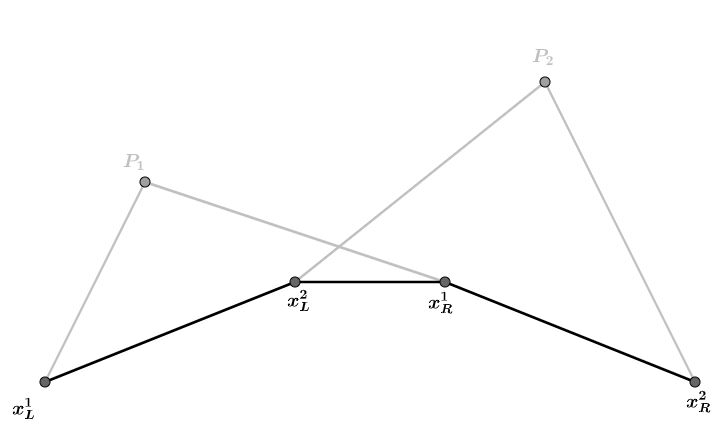
\includegraphics[width = 0.5\linewidth]{proof1_gray.PNG}
\caption{The mothership launches two drones sequentially}
\label{fig:proof1}
\end{figure}


\begin{proof}
Note that in the \EN{configuration considered}, the order of visits to the points $P_1$ and $P_2$ is fixed and then, the binary variables in the model are fixed in this case. Thus, the only differences that the two models can have are the location of the launching and rendezvous points. Hence, the only constraints that are involved are those related to these points. These are the conditions in the statement: The first two are the \eqref{DCW} inequalities. The third is the \eqref{CAP} constraint and the last ensures that the distance traveled by the mothership in the complete overlapping model is smaller than or equal to the distance assumed in the partial overlapping solution described in the statement. Therefore, the conclusion follows.
\end{proof}

\noindent
Note that this result states sufficient conditions to obtain the same solution for the two models.



\color{black}

\section{Strengthening the formulations}\label{bounds}
\noindent
In this section, we present some valid inequalities for \eqref{AMMDRPG} that reinforce the formulation given in Subsection \ref{subsec:CO}. Moreover, the \eqref{DCW} and \eqref{eq:DCW-Overlapping} constraints have products of binary and continuous variables that, when they are linearized, produce bigM constants that have to be tightened. This section also provides some bounds for these constants whenever possible. 



\subsection{Valid inequalities for the \ref{AMMDRPG}}
\noindent
In this problem, we assume that the fleet has more than one drone since otherwise the problem reduces to the \textit{All Terrain Mothership and Drone routing problem with graphs} that was already studied in \cite{art:Amorosi2021}. Therefore, if there exists {an operation} in which more than one drone is launched, the mothership does not need to perform $|\mathcal G|$ different operations. Hence, most likely the model does not need to deal with those operations that are numbered at the end. By exploiting this idea, it is possible to concentrate all drone activities on the first operations, avoiding empty operations in $\mathcal{O}$.
\noindent
Let $\beta^o$ be a binary variable that assumes the value \EN{of} 1 if all the target graphs are visited when the operation $o$ begins, and zero, otherwise. Note that, if all the graphs \EN{have already been} visited before operation $o$ then they are also completed before operation $o+1$. Hence, $\beta$ variables must satisfy the following constraints:

\begin{equation}\tag{Monotonicity}\label{eq:Monotonicity}
\beta^o \leq \beta^{o+1}, \mbox{ for all } o=1,\ldots, |\mathcal{G}|-1.
\end{equation}

\noindent
Let $k^o$ denote the number of graphs that are visited in operation $o$. This number can be computed using the $u$ variables since $u^{e_go}$ takes the value \EN{of} 1 if graph $g$ is visited in operation $o$. Thus:

$$k^o=\sum_{g\in\mathcal G}\sum_{e_g\in E_g} u^{e_go}.$$

\noindent
Hence, if $\beta^o$ equals one, the entire set of graphs in $\mathcal G$ must have been visited before operation $o$:

\begin{equation}\tag{VI-1}\label{eq:VI-1}
\sum_{o'=1}^{o-1} k^{o'} \geq |\mathcal G|\beta^o, \quad\forall o\in\mathcal{O},
\end{equation}
where $|\mathcal G|$ denotes the number of graphs of $\mathcal G$.

\noindent
To reduce the space of feasible solutions, we can assume without loss of generality that it is not permitted to have an operation $o$ without any visiting graphs if some of them are still to be visited. This can be enforced by the following constraints:

\begin{equation}\tag{VI-2}\label{eq:VI-2}
k^o \geq 1 - \beta^o, \quad\forall o\in\mathcal{O}.
\end{equation}

\noindent
The model that we have proposed includes bigM constants. We have defined different bigM constants \EN{throughout} this work. To strengthen the formulations, we provide tight upper and lower bounds for those constants. In this section, we present some results that adjust them for each of the models. The reader may note that the same bounds can be used for both models. Therefore, wlog, we focus on the bigM constants that appear in \eqref{AMMDRPG}.


\subsubsection*{Big $M$ constants bounding the distance from the launching / rendezvous point on the path followed by the mothership to the rendezvous / launching point on the target graph $g\in \mathcal{G}$}


\noindent
To linearize the first addend in \eqref{DCW}, we define the auxiliary non-negative continuous variables $p_L^{e_go}$ (resp. $p_R^{e_go}$) and we model the product by including the following constraints:
\begin{align*}
p_L^{e_go} & \leq  M_L^{e_go}u^{e_go},\\
p_L^{e_go} & \leq d_L^{e_go}, \\
p_L^{e_go} & \geq m_L^{e_go} u^{e_go}, \\
p_L^{e_go} & \geq d_L^{e_go} - M_L^{e_go}(1-u^{e_go}).
\end{align*}
Note that, among all graph nodes and the origin and destination points, it is possible to identify the pair of points at the maximum distance. From this pair of points, we can build a circle whose diameter is the segment joining them. Hence, because we are minimizing the distance traveled by the mothership, every launching  or rendezvous point is inside this circle and the best upper bound $M_L^{e_go}$ or $M_R^{e_go}$ can be described as:

$$
M_R^{e_go} = \max_{\{v\in V_g\cup\{\text{origin}, \text{dest}\}, v'\in V_{g'}\cup\{\text{origin}, \text{dest}\} : g, g'\in\mathcal G\}} \|v - v'\| = M_L^{e_go}.
$$

\noindent
On the other hand, the minimum distance in this case can be zero. This bound is attainable whenever the launching or rendezvous points of the mothership are the same that the rendezvous or launching point on the target graph $g\in \mathcal{G}$.



\subsubsection*{Bounds on the big$M$ constants for the distance from the launching to the rendezvous points on the target graph $g\in \mathcal{G}$.} 
\noindent
When the drone visits a graph $g$, it has to go from one edge $e_g$ to another edge $e'_g$ depending on the order given by $z^{e_ge_g'}$. This fact produces a product of variables linearized by the following constraints:
\begin{align*}
p^{e_ge'_g} & \leq M^{e_ge_g'} z^{e_ge_g'}, \\
p^{e_ge'_g} & \leq d^{e_ge_g'}, \\
p^{e_ge'_g} & \geq m^{e_ge_g'} d^{e_ge_g'}, \\
p^{e_ge_g'} & \geq d^{e_ge_g'} - M^{e_ge_g'}(1-z^{e_ge_g'}).
\end{align*}

\noindent
Since we are taking into account the distance between two edges $e_g=(B^{e_g},C^{e_g}), \, e_g'=(B^{e^\prime_g},C^{e^\prime_g})\in E_g$, the maximum distance between their vertices gives us the upper bound:
\begin{align*}
M^{e_g e^\prime_g} = & \max\{\|B^{e_g} - C^{e^\prime_g}\|, \|B^{e_g} - B^{e^\prime_g}\|, \|C^{e_g} - B^{e^\prime_g}\|, \|C^{e_g} - C^{e'_g}\|\}. 
\end{align*}
We observe that the minimum distance between edges $m^{e_g e^\prime_g}$ can \EN{easily be} obtained computing the minimum distance between two edges, which results in a simple second-order cone program.




\section{A Matheuristic for the Mothership-Drone Routing Problem with Graphs}\label{Math}
\noindent
This section is devoted to present\EN{ing} our matheuristic approach to address the solution of the \AMD. Our motivation comes from the fact that the exact solution of the models presented in Section \ref{Form} is highly time demanding. Alternatively, the matheuristic provides a good quality solution in limited computing times.\\
\noindent
The basic idea of the algorithm is to determine the route that a drone should perform \EN{to visit} each graph $g \in \mathcal{G}$, and thus the entry and exit points $L^{e_{g}}$ and $R^{e^{'}_{g}}$ for each graph.
Sequentially, a clustering procedure on the target graphs is applied to compute the route of the mothership via their reference points and the origin/destination points.
The clustering procedure is based on a random selection of the initial target graphs and for this reason it is repeated a number of times to consider different cluster structures. At each iteration, the new clusters are evaluated by computing the cost of the route visiting their reference points and the origin/destination points. 
The route of minimum length, computed on the reference points of the cluster generated by this iterative procedure, is used to set the values of the binary variables $u^{e_go}$ and $v^{e_go}$, that determines the order of visits to the graphs. Finally, these variables are provided as an initial partial solution to the \AMDCO\xspace model to produce a complete feasible solution.\\
Algorithm \ref{alg:math} reports the pseudocode of this algorithm.

\begin{algorithm}
	\caption{Matheuristic algorithm for \ref{AMMDRPG}}\label{alg:math}
	\KwData{$\mathcal{G}$, $|\mathcal{D}|$, $N_D$, $v_D$, $maxit$ (maximum number of iterations to perform the clustering procedure), $maxseed$ (maximum number of the clustering procedure repetitions)}
	
	STEP 1 (First entry and last exit points for each target graph)\\
	\begin{algorithmic}
		\State For each target graph $g \in \mathcal{G}$, compute the route:\\
		$ L^{e_{g}} \gets \mbox{entry point on $g$ closest to the origin}$\\
		$R^{e^{'}_{g}} \gets \mbox{exit point from $g$ closest to the origin}$\\
		$\mathcal L(e_{g}, e^{'}_{g}) \gets \mbox{route length}$
	\end{algorithmic}
	STEP 2 (Clustering procedure)
	\begin{algorithmic}
		\State $it \gets 1$
		\State $nit \gets 1$
		\State For each target graph $g \in \mathcal{G}$:\;
		$K_g \gets g$ \Comment{one cluster for each target graph}\\
		\While{$nit < maxit$}{
			\State Select randomly two clusters $K_i$ and $K_j$ ($i < j$)\\
			\If{$| K_i \cup K_j | < |\mathcal{D}|$}
			{
				\State Search for point $P$ satisfying the following endurance constraint:\\
				\begin{equation}
					\frac{d(P, R^{e_g}) + \mathcal L(e_{g}, e^{'}_{g}) + d(L^{e^{'}_{g}}, P)}{v_D} \leq N_D, \quad \forall R^{e_g}, L^{e^{'}_{g}} \in K_i, \:\: K_j. \label{eq:endurance_math}
				\end{equation}
				\If{$P \:\: \exists$}{\State $K_i \gets K_i \cup K_j$}
			}
			\State $nit \gets nit +1$
		}
		$\mathcal K \gets \mbox{set of clusters}$
	\end{algorithmic}
	STEP 3 (Computation of Reference Points) 
	\begin{algorithmic}
		\State For each cluster $K_i \in \mathcal K$\;
		compute a reference point $P_i$ by solving the following minimization problem:
		$$
		\min \sum_{K_i \in \mathcal K}( \|P_i - origin\| + \|P_i - dest \|) + \sum_{g \in K_i: K_i \in \mathcal K} (\|P_i - R^{e_g} \| + \| P_i - L^{e'_g}\|) + \sum_{K_i, K_j \in \mathcal K: i \neq j} \|P_i - P_j\|
		$$
		subject to (\ref{eq:endurance_math}).
	\end{algorithmic}
	STEP 4 (Order of visits to the graphs: route via the reference points and the origin/destination points)
	\begin{algorithmic}
		\State Compute the TSP of the mothership among the reference points $P_i$ of the clusters\\
		\State \CV{$\mathcal L(TSP) \gets \mbox{TSP length}$} [This update is performed only if $\mathcal L(TSP)$ decreases with respect to the previous iteration $it - 1$]
		\State $it \gets it+1$\\
		\eIf{$it < maxseed$}{go to STEP 2}{go to STEP 5}
	\end{algorithmic}
	STEP 5 (Solution of the \AMD\xspace model by fixing an initial partial solution)
	\begin{algorithmic}
		\State Set the initial values of the binary variables $u^{e_{g}o}$ and $v^{e_{g}o}$ and solve the model \CV{\AMD}\xspace to obtain a feasible solution.
	\end{algorithmic}
	\KwResult{Feasible solution for \CV{\ref{AMMDRPG}}}
\end{algorithm}


\noindent




\begin{figure}[h]
\centering
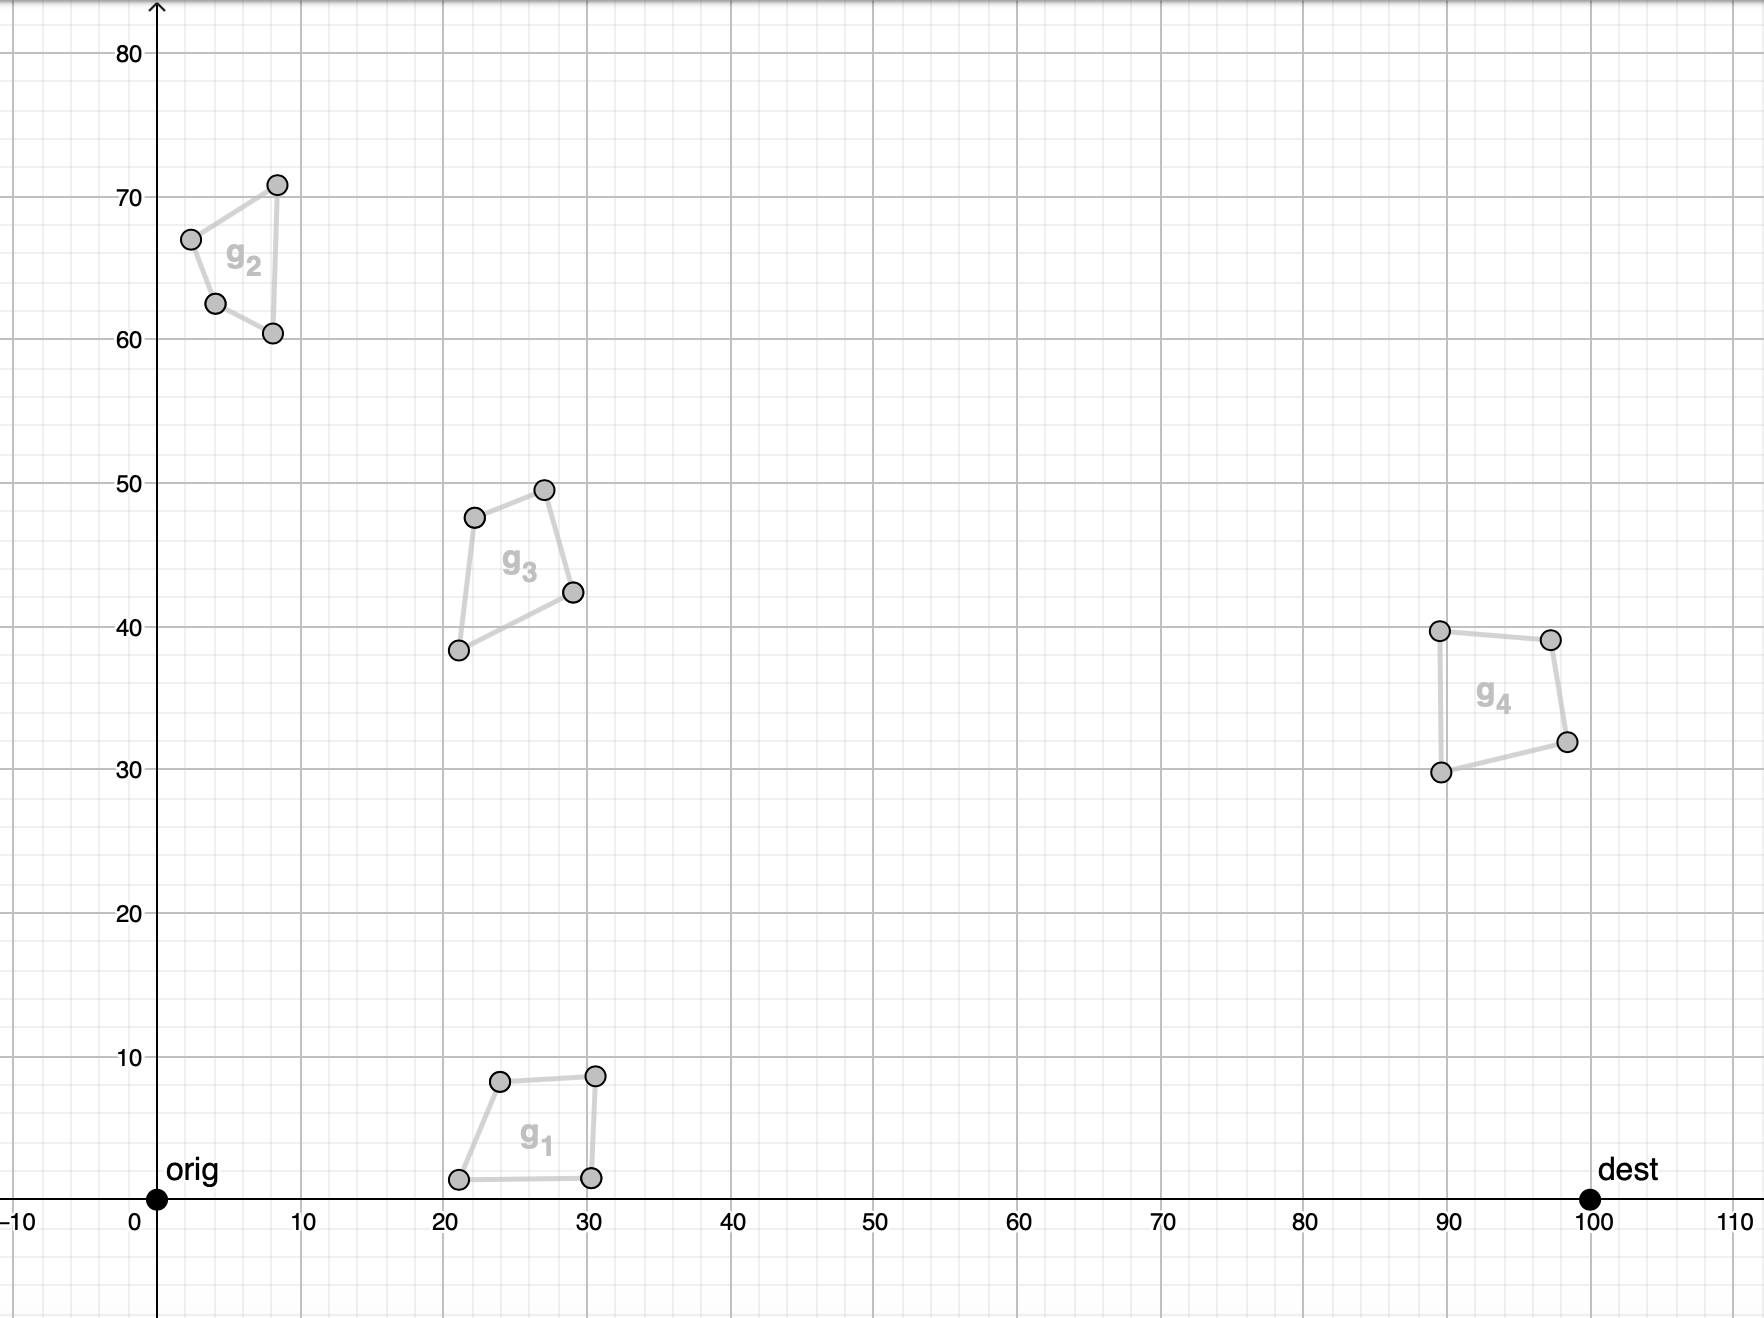
\includegraphics[width = 0.5\linewidth]{example_new_gray.png}
\caption{Illustrative example \label{fig:example1}}
\end{figure}

\noindent
Figure \ref{fig:example1} shows an illustrative example consisting of four target planar graphs ($g_1$, $g_2$, $g_3$ and $g_4$) to be visited. We assume that their visits must be performed by a fleet of two drones supported by a mothership whose path starts from the origin $(0,0)$ and ends \EN{at} the destination point $(100,0)$.



\begin{figure}[h!]
	\centering
\begin{subfigure}[b]{.35\textwidth}
	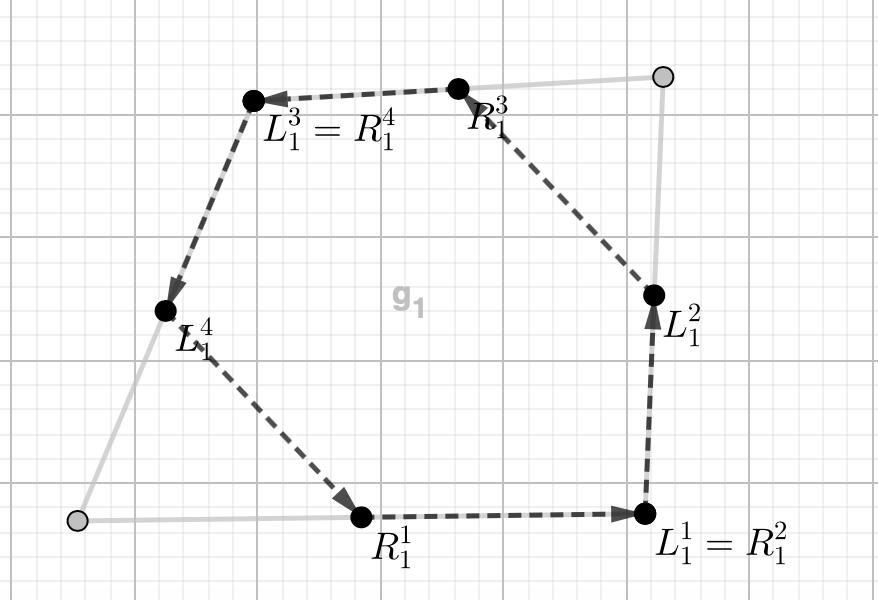
\includegraphics[width=\textwidth]{example_tour_g1_Step1_new_gray.png}
	\caption{}
\end{subfigure}
\begin{subfigure}[b]{.35\textwidth}
	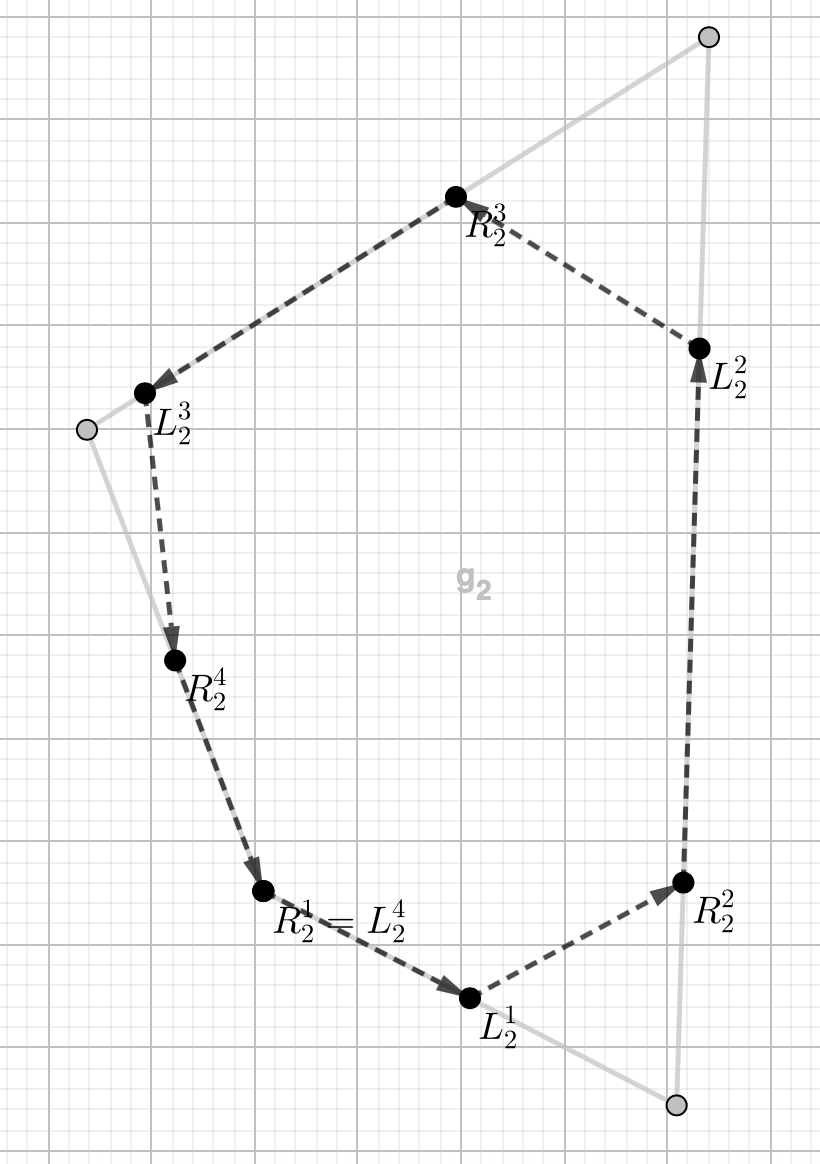
\includegraphics[width=\textwidth]{example_tour_g2_Step1_new_gray.png}
	\caption{}
\end{subfigure}
\begin{subfigure}[b]{.35\textwidth}
	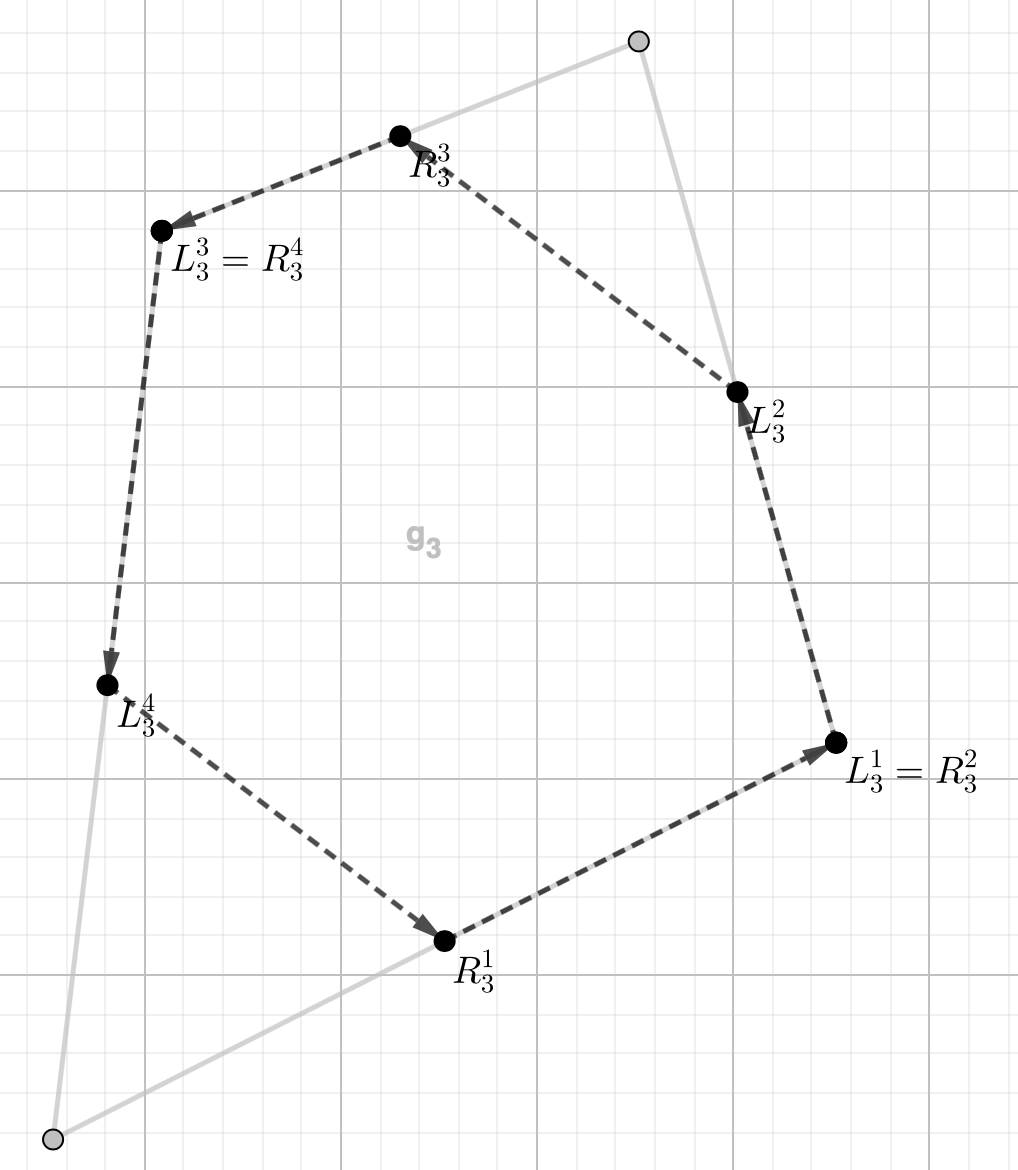
\includegraphics[width=\textwidth]{example_tour_g3_Step1_new_gray.png}
	\caption{}
\end{subfigure}
\begin{subfigure}[b]{.35\textwidth}
	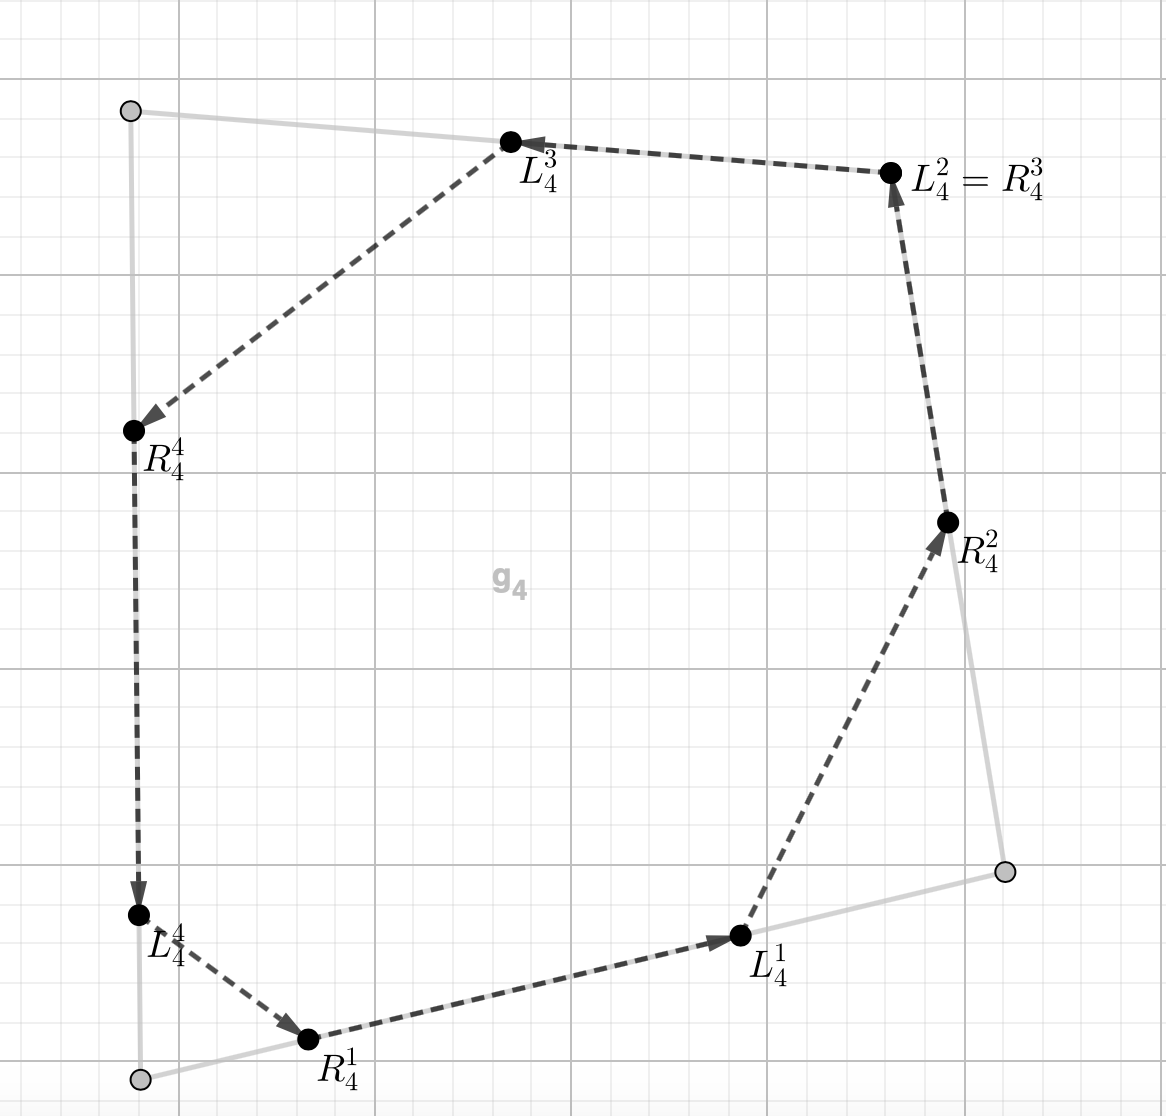
\includegraphics[width=\textwidth]{example_tour_g4_Step1_new_gray.png}
	\caption{}
\end{subfigure}
\caption{STEP 1 for the illustrative example}%
\label{fig:example2}%
\end{figure}

\noindent
Figure \ref{fig:example2} \EN{illustrates} a zoom \EN{in} on each single target graph, showing the tours generated by STEP 1 of the matheuristic procedure. A pair of points representing retrieving and launching points,  together with an arrow pointing the direction followed by the drone according to the order in which the edges are visited, are depicted on each edge.

\begin{figure}[h!]
	\centering
	\begin{subfigure}[b]{.4\textwidth}
		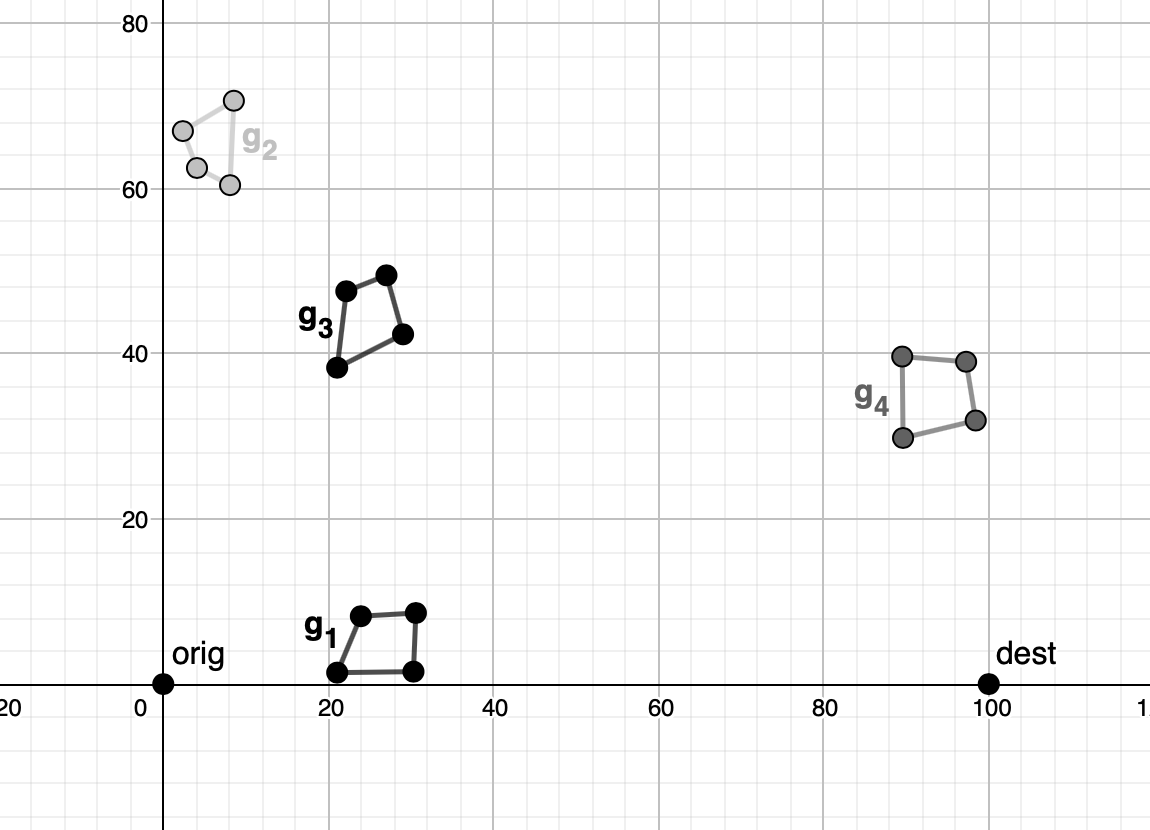
\includegraphics[width=\textwidth]{example_step2_new_gray.png}
		\caption{}%
	\end{subfigure}
	\begin{subfigure}[b]{.4\textwidth}
		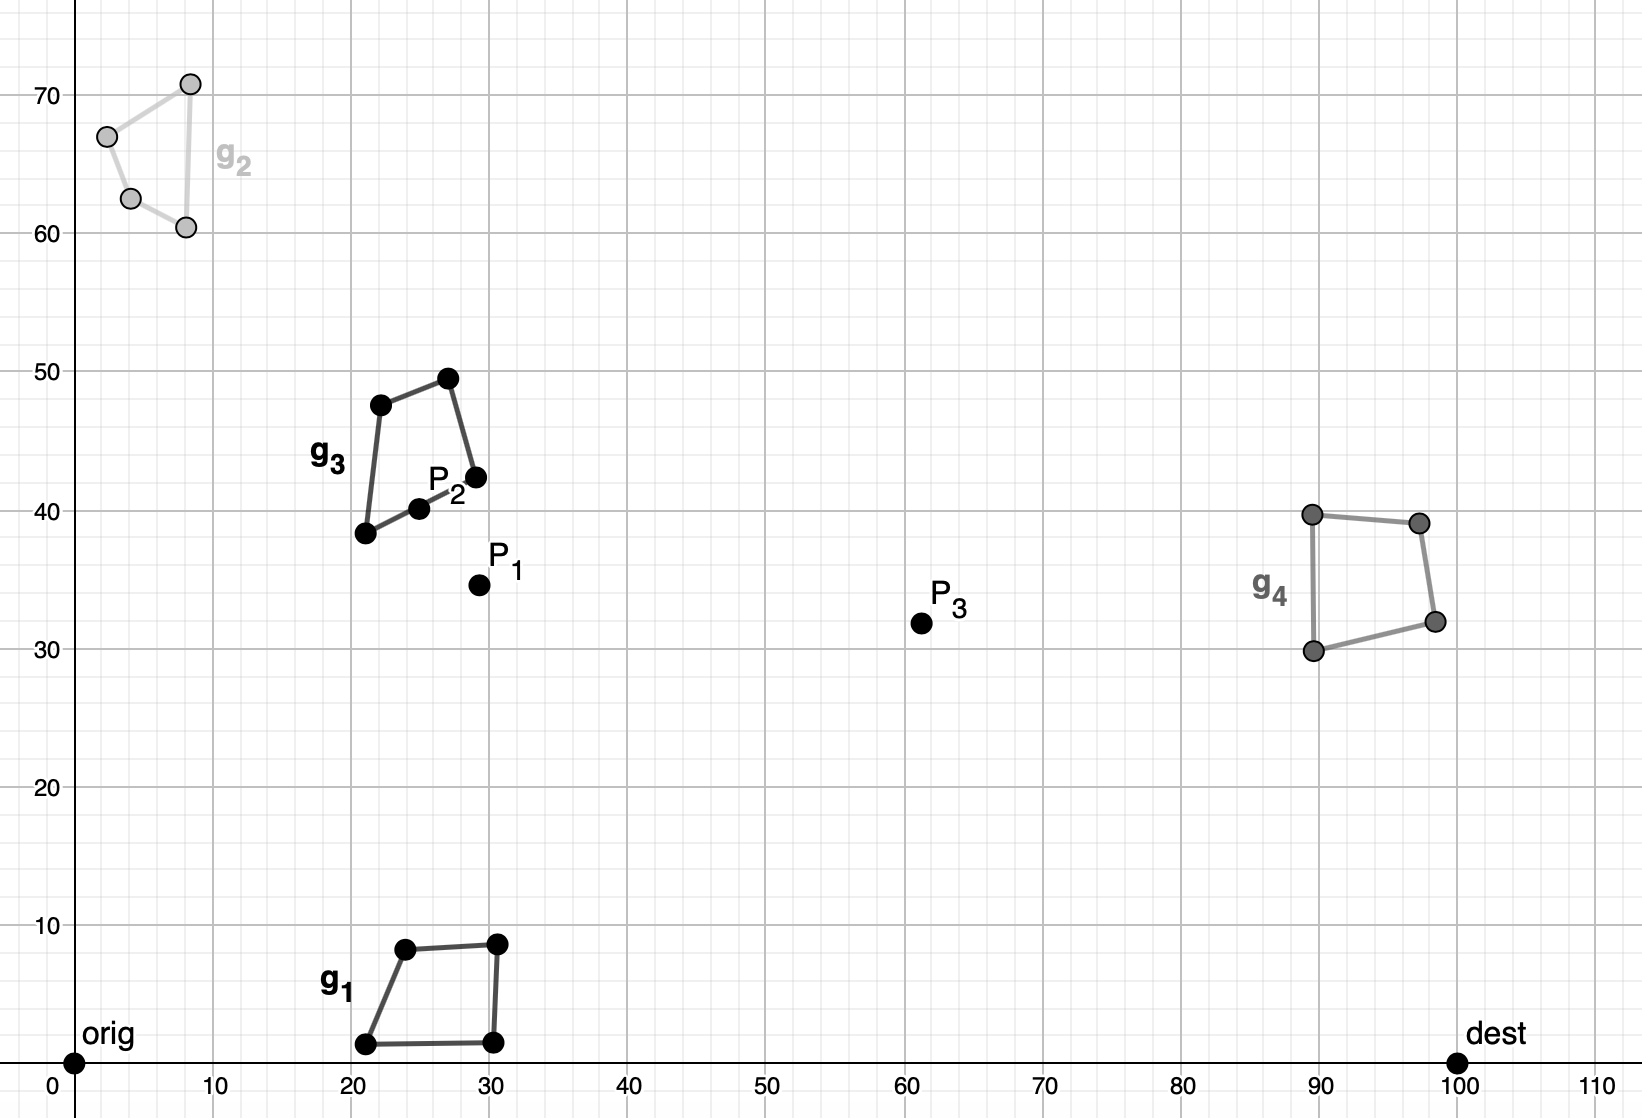
\includegraphics[width=\textwidth]{example_step3_new_gray.png}
		\caption{}%
	\end{subfigure}
	\caption{(a) STEP 2, (b) STEP 3 for the illustrative example}%
	\label{fig:example3}%
\end{figure}

\noindent
By applying STEP 2 to this illustrative example, we obtain three clusters, as shown in Figure \ref{fig:example3}(a). One cluster contains graphs $g_1$ and $g_3$ (in black), while graph $g_2$ and $g_4$ represent distinct clusters. The computation of the reference points of these clusters, according to STEP 3, produces the points $P_1$, $P_2$ and  $P_3$, as shown in Figure  \ref{fig:example3}(b).


\begin{figure}[h!]
	\centering
	\begin{subfigure}[b]{0.4\textwidth}
		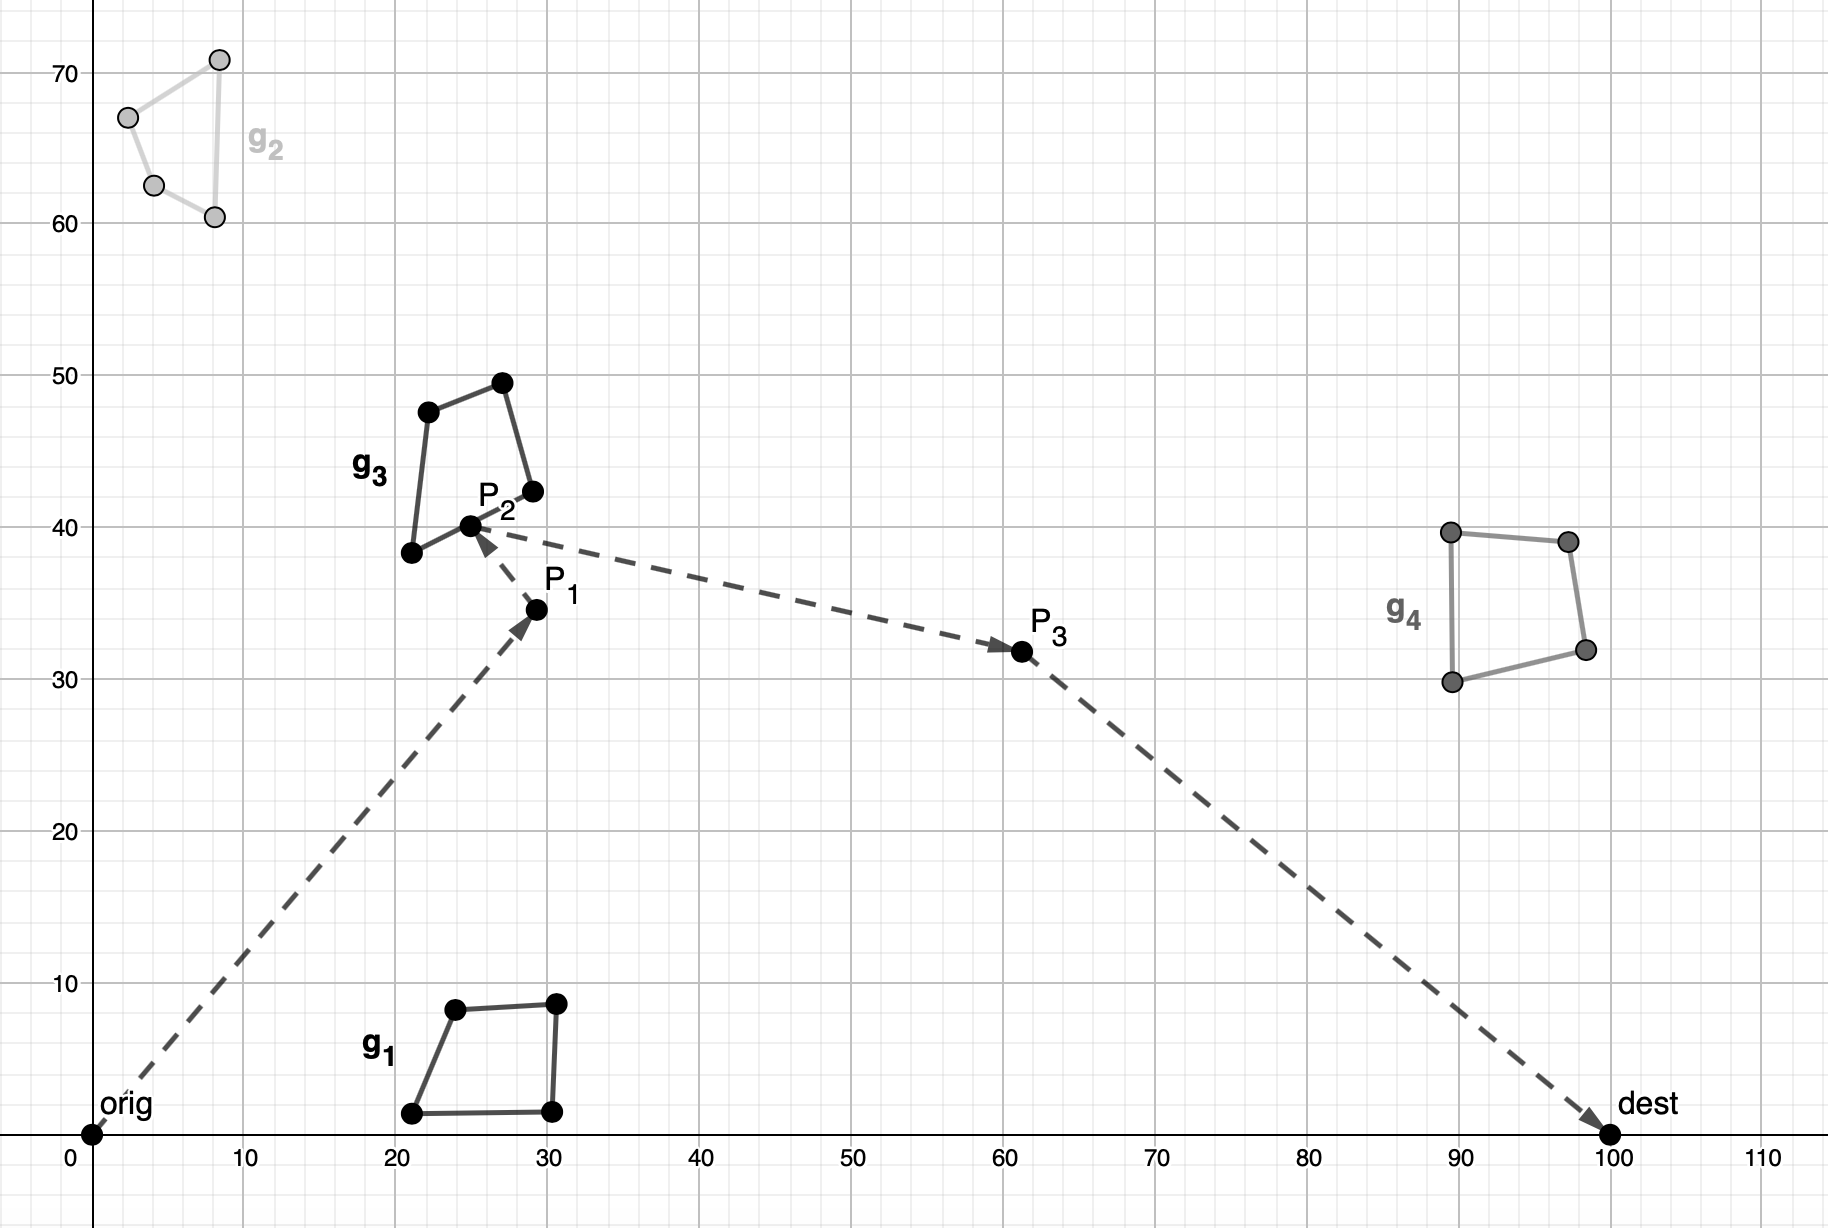
\includegraphics[width=\textwidth]{example_step4_new_gray.png}
		\caption{}%
	\end{subfigure}
	\begin{subfigure}[b]{0.4\textwidth}
		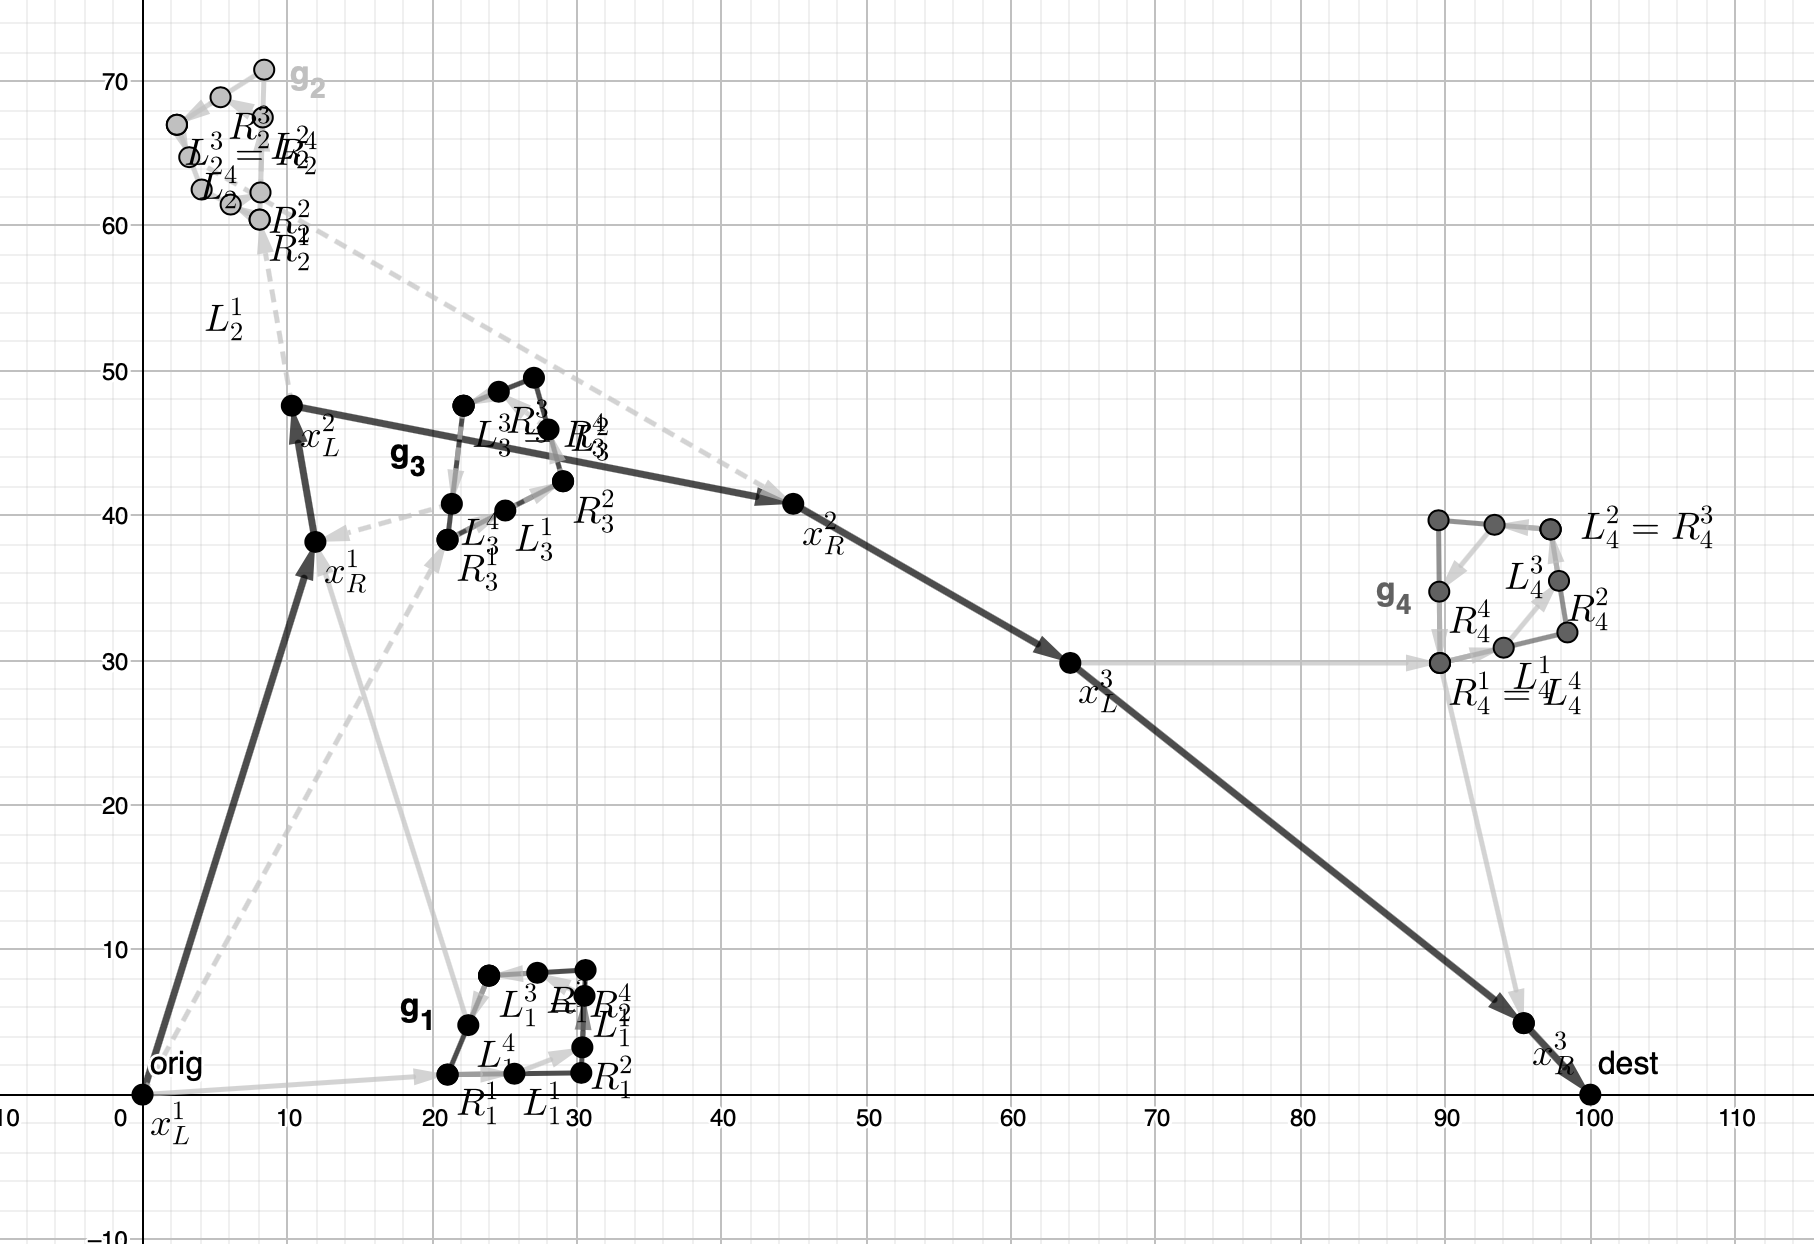
\includegraphics[width=\textwidth]{example_step5_new_gray.png}
		\caption{}
	\end{subfigure}%
	\caption{(a) STEP 4, (b) STEP 5 for the illustrative example}%
	\label{fig:example4}%
\end{figure}

\noindent
STEP 4 of the matheuristic procedure generates the tour of the mothership along the origin point, $P_1$, $P_2$, $P_3$ and the destination point, as shown in Figure \ref{fig:example4}(a). This tour \EN{also returns} the order in which the clusters are visited (and thus, also the order of visits to the target graphs) and this permits \EN{us} to set the values of the variables $u^{e_{g}o}$ and $v^{e_{g}o}$ of the \AMD\space model.\\
\noindent 
By providing the initial partial solution obtained \EN{from} the values of the variables $u^{e_{g}o}$ and $v^{e_{g}o}$, STEP 5 solves the \AMD\space model and returns the final feasible solution shown in Figure \ref{fig:example4}(b). From it, we can observe that the sequence of visits \EN{to} the target graphs does not change with respect to \EN{that} provided by STEP 4. The fleet of two drones first visits the graphs $g_1$ and $g_3$ starting from the launching point $x^1_L$. Then, both drones are retrieved by the mothership at point $x^1_R$. The mothership moves to the point $x^2_L$  where one drone is launched \EN{to visit} graph $g_2$. Then the mothership reaches the point $x^2_R$ to retrieve the drone and from the same point it launches the other drone \EN{to visit} graph $g_4$. Then, this drone is retrieved by the mothership at point $x^3_R$ before moving to the final destination point.


\begin{figure}[h!]
	\centering
	\begin{subfigure}[b]{0.4\textwidth}
		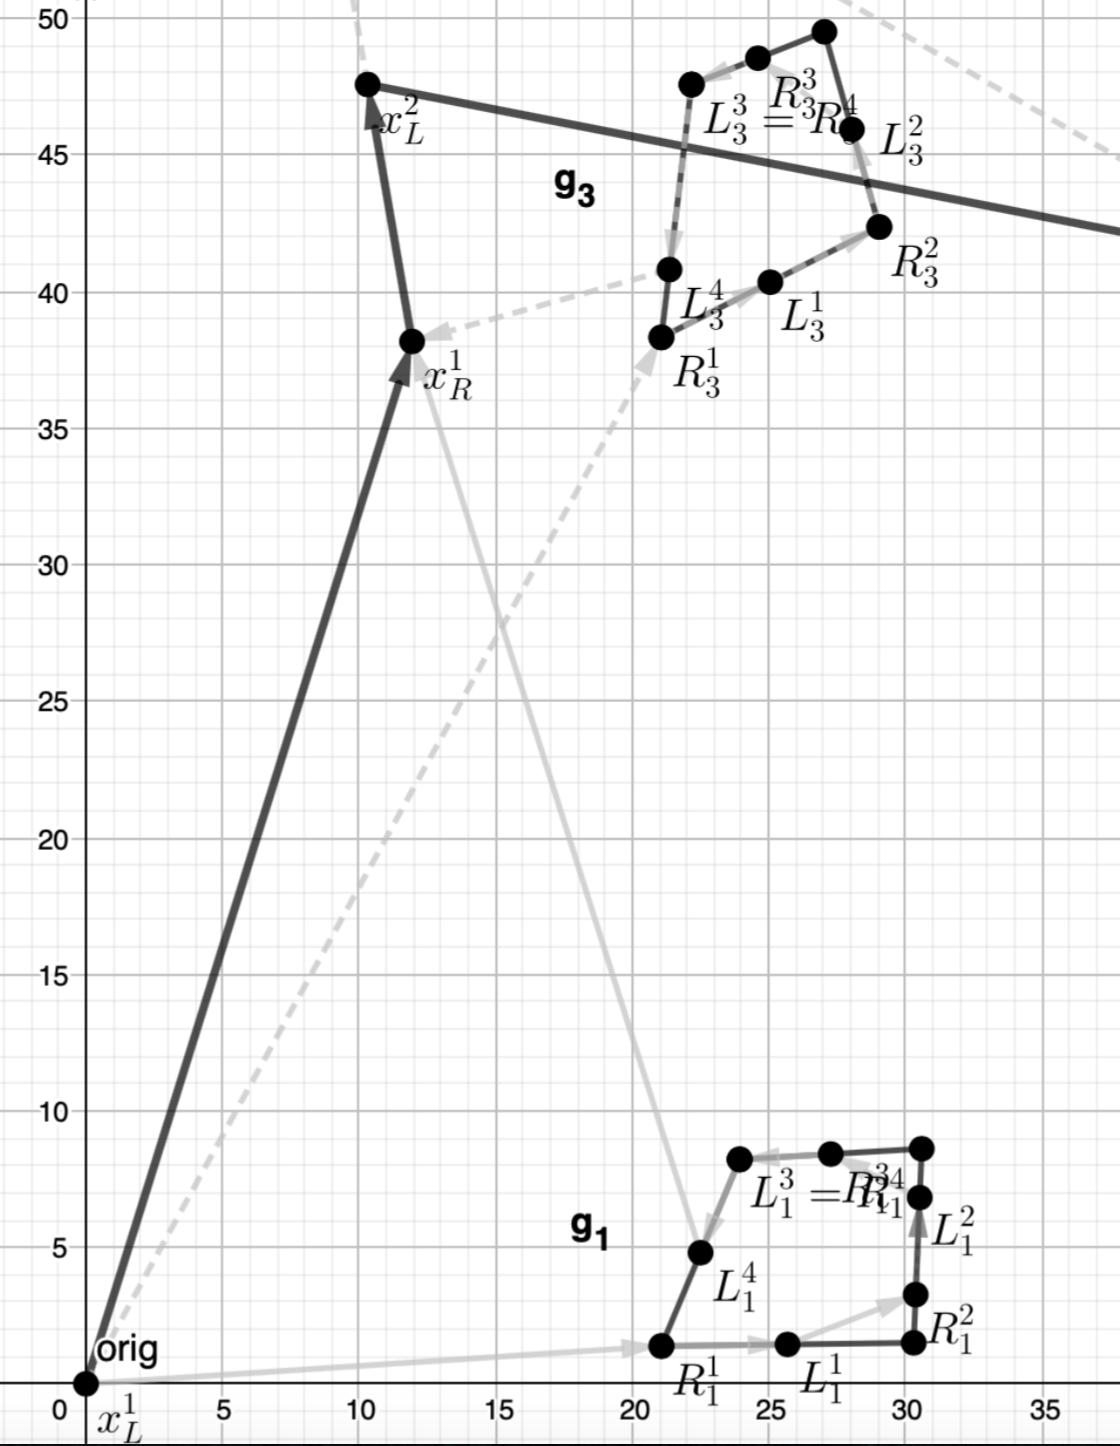
\includegraphics[width=\textwidth]{example_final-g1_g3_gray.png}%
		\caption{}
	\end{subfigure}
	\begin{subfigure}[b]{0.4\textwidth}
		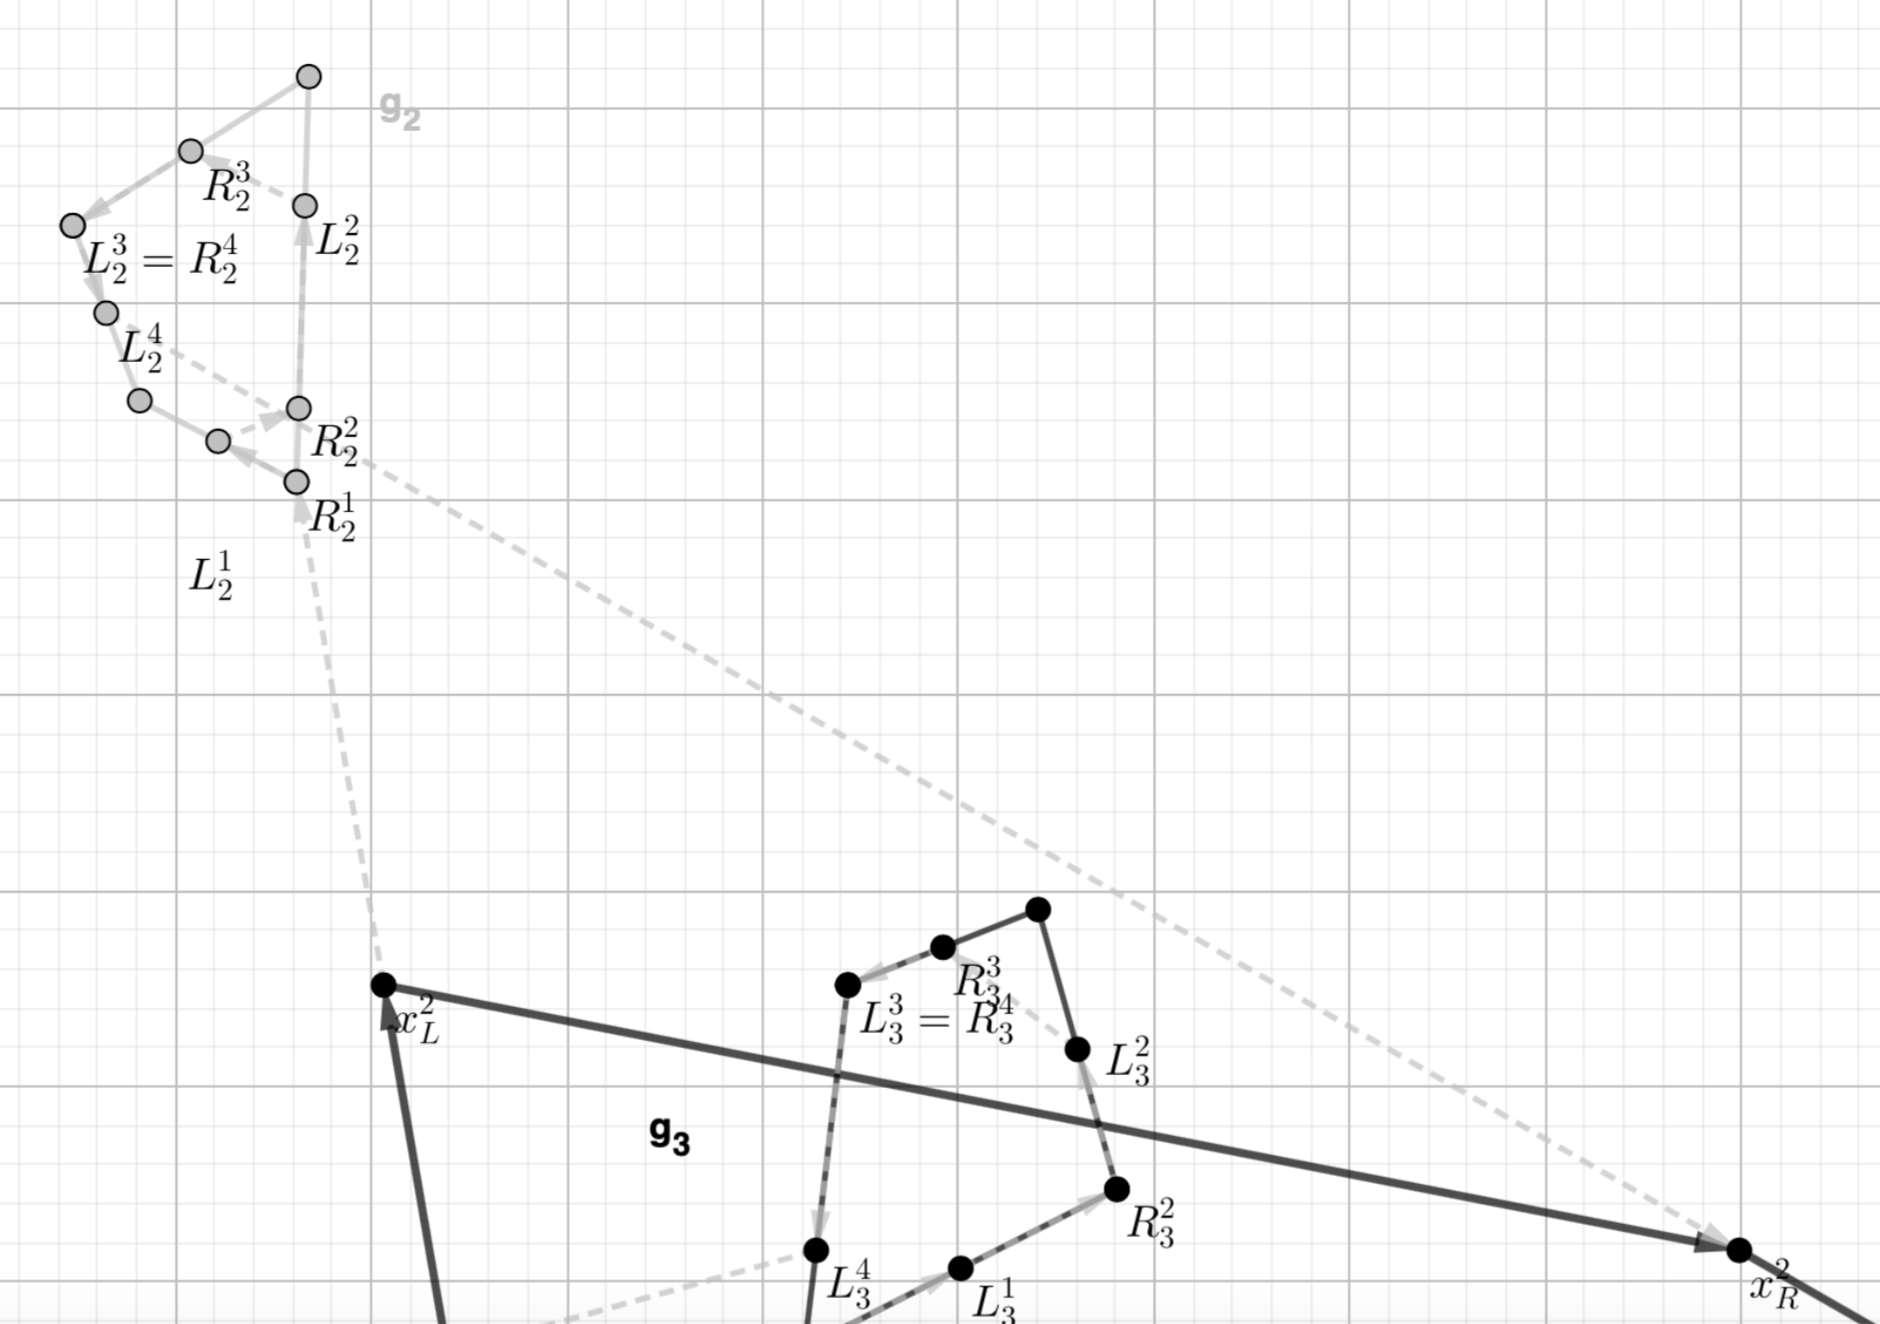
\includegraphics[width=\textwidth]{example_final-g2_gray.png}
		\caption{}%
	\end{subfigure}
	\begin{subfigure}[b]{0.4\textwidth}
		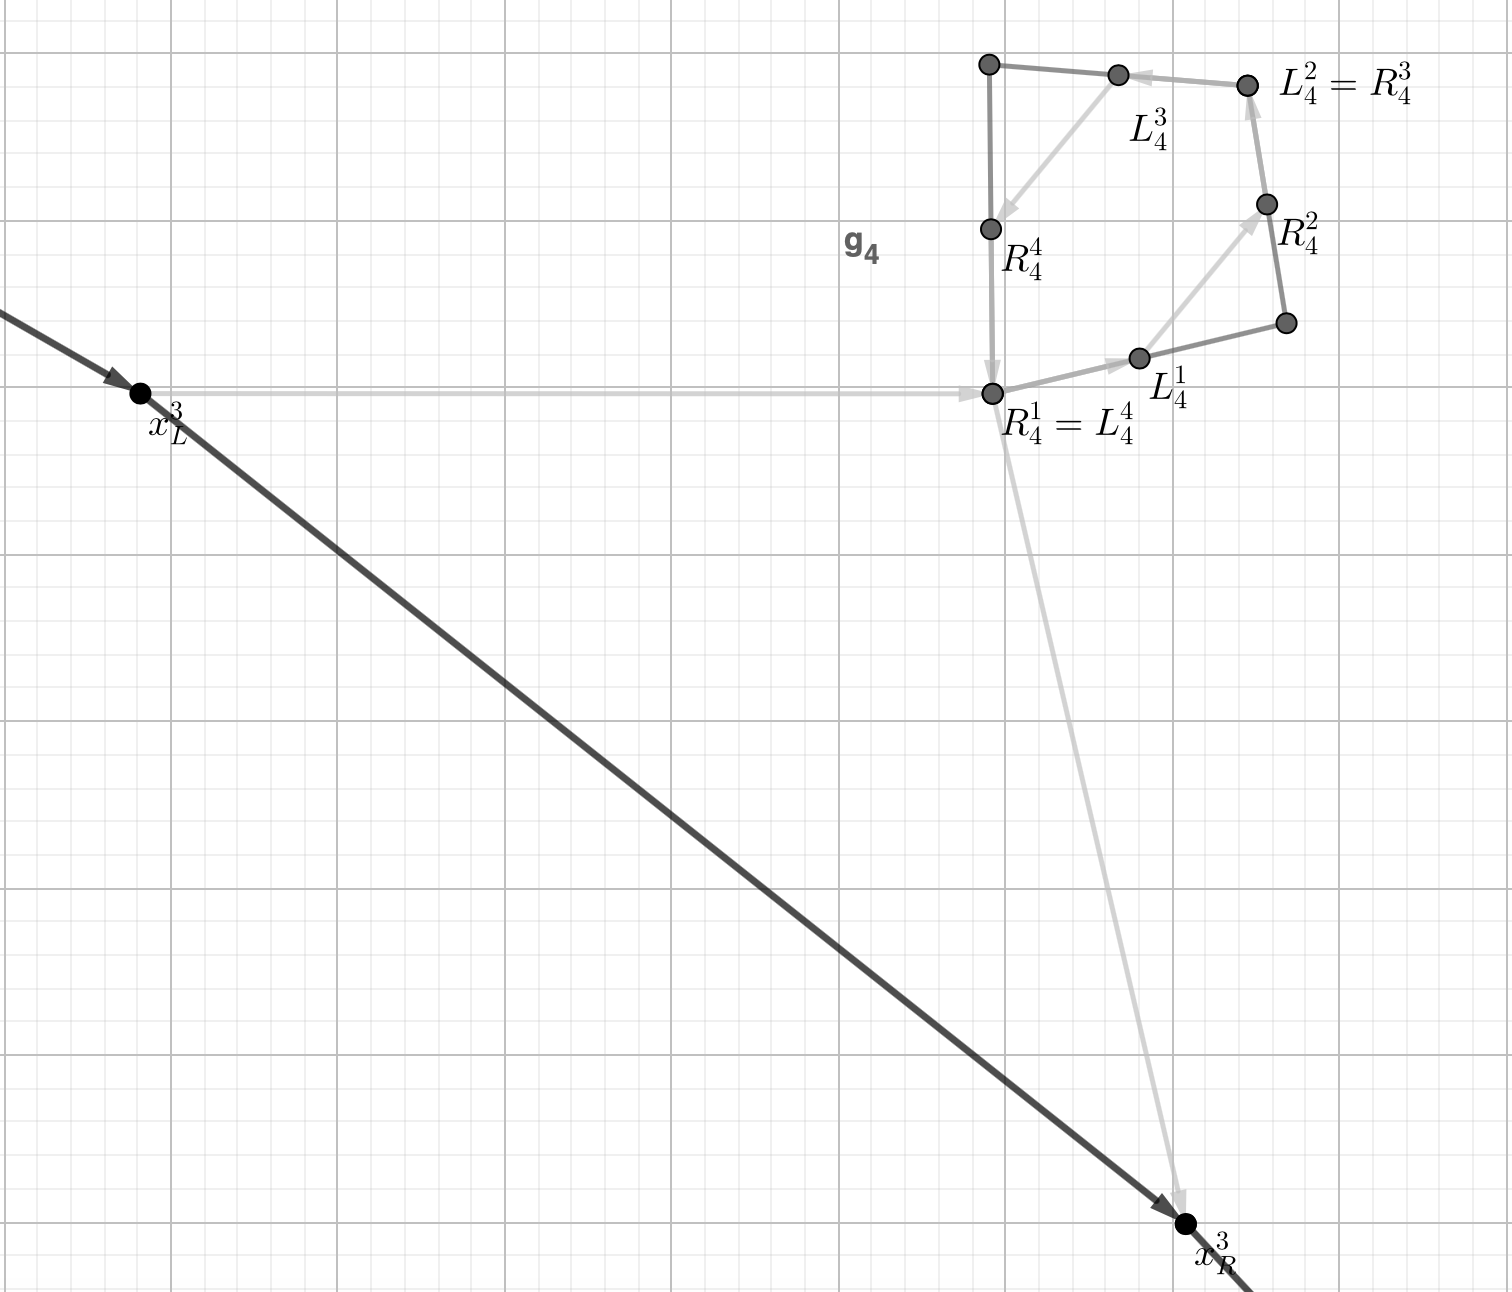
\includegraphics[width=\textwidth]{example_final-g4_gray.png}
		\caption{}
	\end{subfigure}%
	\caption{Zoom on the tour on each target graph provided by STEP 5}%
	\label{fig:example5}%
\end{figure}

\noindent 
Focusing on each single target graph, Figure \ref{fig:example5} shows the zoom \EN{in} on the tours followed by the drones. For example, Figure \ref{fig:example5}[a] reports th\EN{at} performed by the drone that visits the graph $g_1$ (the gray segments) and the drone that visits the graph $g_3$ (the dotted gray segments). Both drones start from the mothership at point $x^1_L$ that is the $origin$. One drone first visits the segment $\overline{R^1_1L^1_1}$ of the graph $g_1$, while the other starts the visit \EN{to} graph $g_3$ by traversing the segment $\overline{R^3_1L^3_1}$. From point $L^1_1$ the first drone moves to the second visited edge of the graph $g_1$ by traversing the segment $\overline{R^2_1L^2_1}$. Then, it moves to the third visited edge of graph $g_1$, by flying over the segment $\overline{R^3_1L^3_1}$. From point $R^4_1$ the drone starts the visit to the last edge of graph $g_1$ up to point $L^4_1$. 
Finally, the drone leaves graph $g_1$ at this latter point and is retrieved by the mothership at point $x^1_R$. Similarly, the second drone, that visits graph $g_3$, after traversing segment $\overline{R^1_3L^1_3}$, moves to the second visited edge of the same graph and traverses segment $\overline{R^2_3L^2_3}$. Then, it flies to the third visited edge, by traversing segment $\overline{R^3_3L^3_3}$. Finally it moves to the last visited edge of the graph $g_3$, by flying over segment $\overline{R^4_3L^4_3}$. The drone leaves graph $g_3$ at point $L^4_3$ and reaches the mothership at point $x_R^1$. 
Note that in this example the drones do not visit the full 100\% of each graph edge, but only half of each of them.

\bigskip
\noindent
The reader may notice that the \EN{algorithm above} can \EN{also be} used to generate solutions for the partial overlapping model presented in Section \ref{amdasyn} since any solution of the \AMDCO\xspace model is also feasible for the \AMDPO\xspace one as shown in Theorem \ref{th:relaxation}.





\section{Experimental results\label{section:results}}



\noindent
In this section, we discuss the experimental results obtained testing the formulations presented in Section \ref{Form} and the matheuristic procedure proposed in Section \ref{Math} on a testbed of instances. In particular, we consider instances like the ones used in \cite{art:Amorosi2021}, where the targets to be visited by the drones are represented by grid graphs.
We generated one set of 5 instances with 5 graphs and another set of 5 instances with 10 graphs. More precisely, each instance is composed of 20$\%$ graphs with 4 nodes, 20$\%$ graphs of 6 nodes, 20$\%$ graphs of 8 nodes, 20$\%$ graphs of 10 nodes and and 20$\%$ graphs with 12 nodes. Moreover, we assume that the velocity of the drones is twice that of the mothership and that a random fraction of each target graph, or of each of its edges, must be visited by the fleet of drones. These fractions are uniform\EN{ly} randomly sampled in the interval $(0, 1)$.\\

\noindent
We consider in our experiments that the number of drones varies between 1 and 3 and that the drone endurance (expressed as the maximum time that the drone can operate when it is fully recharged) ranges between 20 and 60. Note that the case of a single drone is also included in our experiments to compare the results and complexity of using one \EN{or} more than one drone. The interested reader is referred to \cite{art:Amorosi2021} \EN{to analyze} the complexity in terms of gap of the model with a single drone.
Table \ref{table:tab1} reports a summary of the characteristics of our instances.

\renewcommand{\arraystretch}{0.7}
\begin{table}[!h]
\caption{Instance parameter values}
\centering
\footnotesize
\begin{tabular}{c | c }
	\hline
	$|\mathcal G|$ & (5,10)\\
	\hline
	$|\mathcal D|$ &	(1,2,3)\\
	\hline
	$|V_g|$ & (4,6,8,10,12)\\
	\hline
	$N_D$ & (20,30,40,50,60)\\
	\hline
	fraction target (edge) & uniform\EN{ly} randomly sampled in $(0, 1)$.
\end{tabular}
\label{table:tab1}
\end{table}

\noindent
We coded the matheuristic and the exact resolution of the model in Python 3.8.10. The mathematical programming formulation \EN{was} implemented in Gurobi 9.1.2. All the tests \EN{were} run on a machine AMD® Epyc 7402p with 24-core processor × 8.
Table \ref{table:tab2} reports the results obtained solving both variants of the \AMD\xspace model on the instances previously described, by adopting the commercial solver Gurobi. We consider the exact solution both providing and not providing an initial solution computed by the matheuristic described in Section \ref{Math}. More precisely, the first row of Table \ref{table:tab2} indicates the model variant and the second row reports the number of target graphs to be visited by the fleet of drones (5 or 10). From the third row, we split each column in\EN{to} three sub-columns. The first three sub-columns report respectively, the endurance of the drones, the size of the fleet of drones and \EN{an} indication \EN{of} the visit of a fraction of each edge (e) or a fraction of each target graph (g). From sub-column 4 to sub-column 15, we report, for each combination of the listed parameters characterizing the instances, respectively, the average gap without initialization by the solution provided by the matheuristic (wi), the average gap with initialization by the solution obtained by the matheuristic (i) and the solution time, in seconds, of the matheuristic (TimeH). The time limit of these experiments is set equal to 1 hour.\\
\noindent
We can observe that the value of the average percentage gap ranges between a minimum of 58\% and a maximum of 100\%. This shows that the model is hard \EN{to solve} even with small size instances. Moreover, we can see that for the complete overlapping version of the model, in most cases, the average gap associated with the variant of the model consisting \EN{of} visiting a given fraction of each edge, is higher than \EN{that} associated with the variant \EN{obligating} to visit a given fraction of each target graph. 
Another thing that we can observe is that the average percentage gap increases with the number of target graphs for both problem variants.\\
\noindent
Moreover, the reader may note that the partial overlapping version of the problem is harder to solve than the complete overlapping version by looking at the values of the average gap. This is an expected \EN{behavior} due to the fact that the feasible region of the partial overlapping variant contains the one associated with the complete overlapping variant, as proven in Theorem \ref{th:relaxation}. 
We can see that for both versions of the problem, by increasing the number of target graphs from 5 to 10, the exact method without initialization of the solution obtained with the matheuristic, becomes even harder. Indeed, the gray entries of the table mean that some instances could not find a feasible solution within the time limit (note that in the brackets we indicate the number of these instances). 
\EN{Furthermore}, for the minimum level of endurance, the exact solution of the partial overlapping model without initialization provided by the matheuristic, does not find any solution within the time limit for instances with 10 graphs, 3 drones and a given fraction of each edge to be visited. The same can \EN{also} be observed for the exact solution of the complete overlapping model without initialization provided by the matheuristic, for a level of endurance equal to 30, a fleet of 3 drones and a given fraction of each edge to be visited.\\
Considering the comparison with the exact method starting from the solution provided by the matheuristic, we can note that the values of the average percentage gap are very close to \EN{those} related to the exact solution method without initialization. Thus, the initialization does not speed up the convergence of the solver. However, we can see that the matheuristic is always able to find a feasible solution \EN{to} the problem, even for the cases in which the solver is not. 


\noindent
Furthermore, the average solution times of the matheuristic range between a minimum of 4 seconds to a maximum of 9.5 minutes. In particular, we can observe that, in most cases, for the complete overlapping version of the problem, the matheuristic running time is shorter for the instances where a fraction of the length of each graph is required to be visited. The same \EN{behavior} can be noticed for the partial overlapping version of the problem for which the difference in terms of running time is even bigger. Indeed, when a given fraction of the length of each edge is required, STEP 1 of the matheuristic (computation of the TSP over the graph edges) takes more time. By increasing the number of target graphs from 5 to 10, the average solution times of the matheuristic increases for both model variants.
Summing up, the results obtained show that the exact solution method given by solving the formulation is very challenging even for small size instances. However, exploiting it, the matheuristic is able to provide  solutions for all instances \EN{quite} quickly.

\begin{table}[h!]
\centering
\caption{Comparison between the partial and complete overlapping models}
\resizebox{\textwidth}{!}{
\begin{tabular}{|c|c|c||ccc|ccc||ccc|ccc|}
\hline
\multicolumn{3}{|c|}{\textbf{Model}} & \multicolumn{6}{c|}{Complete Overlapping}     & \multicolumn{6}{c|}{Partial Overlapping} \bigstrut\\
\hline
\multicolumn{3}{|c|}{$|\mathcal G|$} & \multicolumn{3}{c|}{5} & \multicolumn{3}{c|}{10} & \multicolumn{3}{c|}{5} & \multicolumn{3}{c|}{10} \bigstrut\\
\hline
$N_D$ & $|\mathcal D|$ & $\alpha$ & Gap (wi) & Gap (i) & TimeH & Gap (wi) & Gap (i) & TimeH & Gap (wi) & Gap (i) & TimeH & Gap (wi) & Gap (i) & TimeH \bigstrut\\
\hline
\hline
\multirow{6}[6]{*}{20} & \multirow{2}[2]{*}{1} & g     & 0.78  & 0.79  & 6.01  & \textcolor[rgb]{ 1,  0,  0}{0.91 (2)} & 0.86  & 177.69 & 0.65  & 0.63  & 16.53 & 1     & 1     & 215.59 \bigstrut[t]\\
&       & e     & 0.81  & 0.81  & 15.41 & \textcolor[rgb]{ 1,  0,  0}{0.89 (2)} & 0.84  & 148.95 & 0.84  & 0.83  & 52.36 & \textcolor[rgb]{ 1,  0,  0}{0.88 (3)} & 0.87  & 440.93 \bigstrut[b]\\
\cline{2-15}          & \multirow{2}[2]{*}{2} & g     & 0.81  & 0.87  & 5.76  & \textcolor[rgb]{ 1,  0,  0}{0.96 (3)} & 0.96  & 139.24 & 0.97  & 0.96  & 13.91 & \textcolor[rgb]{ 1,  0,  0}{1 (3)} & 1     & 76.77 \bigstrut[t]\\
&       & e     & 0.93  & 0.92  & 33.99 & \textcolor[rgb]{ 1,  0,  0}{0.97 (3)} & 0.97  & 163.41 & \textcolor[rgb]{ 1,  0,  0}{0.86 (2)} & 0.85  & 66.38 & \textcolor[rgb]{ 1,  0,  0}{0.89 (4)} & 0.85  & 578.31 \bigstrut[b]\\
\cline{2-15}          & \multirow{2}[2]{*}{3} & g     & 0.88  & 0.89  & 4.83  & \textcolor[rgb]{ 1,  0,  0}{0.95 (3)} & 0.94  & 67.76 & 0.97  & 0.97  & 17.87 & \textcolor[rgb]{ 1,  0,  0}{1 (2)} & 1     & 18.88 \bigstrut[t]\\
&       & e     & 0.92  & 0.91  & 14.08 & \textcolor[rgb]{ 1,  0,  0}{0.97 (2)} & 0.97  & 125.89 & \textcolor[rgb]{ 1,  0,  0}{0.81 (3)} & 0.84  & 61.83 & \textcolor[rgb]{ 1,  0,  0}{- (5)} & 0.82  & 237.33 \bigstrut[b]\\
\hline
\hline
\multirow{6}[6]{*}{30} & \multirow{2}[2]{*}{1} & g     & 0.71  & 0.7   & 9.66  & \textcolor[rgb]{ 1,  0,  0}{0.82 (4)} & 0.82  & 87.4  & 0.77  & 0.75  & 15.43 & 1     & 1     & 39.83 \bigstrut[t]\\
&       & e     & 0.79  & 0.8   & 14.16 & \textcolor[rgb]{ 1,  0,  0}{0.8 (4)} & 0.83  & 122.23 & 0.84  & 0.82  & 38.94 & \textcolor[rgb]{ 1,  0,  0}{0.83 (4)} & 0.81  & 289.74 \bigstrut[b]\\
\cline{2-15}          & \multirow{2}[2]{*}{2} & g     & 0.82  & 0.82  & 4.98  & \textcolor[rgb]{ 1,  0,  0}{0.95 (3)} & 0.92  & 174.64 & 0.97  & 0.96  & 12.94 & 1     & 1     & 45.37 \bigstrut[t]\\
&       & e     & 0.84  & 0.84  & 14.73 & \textcolor[rgb]{ 1,  0,  0}{0.96 (3)} & 0.97  & 133.75 & 0.78  & 0.79  & 31.82 & 0.82  & 0.77  & 171.16 \bigstrut[b]\\
\cline{2-15}          & \multirow{2}[2]{*}{3} & g     & 0.82  & 0.81  & 4.63  & \textcolor[rgb]{ 1,  0,  0}{0.93 (3)} & 0.95  & 105.54 & 0.96  & 0.96  & 16.22 & 1     & 1     & 33.95 \bigstrut[t]\\
&       & e     & 0.88  & 0.89  & 12.08 & \textcolor[rgb]{ 1,  0,  0}{- (5)} & 0.97  & 127.78 & 0.83  & 0.82  & 35.38 & \textcolor[rgb]{ 1,  0,  0}{0.79 (3)} & 0.8   & 213.06 \bigstrut[b]\\
\hline
\hline
\multirow{6}[6]{*}{40} & \multirow{2}[2]{*}{1} & g     & 0.68  & 0.68  & 5.79  & \textcolor[rgb]{ 1,  0,  0}{0.81 (2)} & 0.82  & 93.21 & 0.73  & 0.71  & 11.46 & 1     & 1     & 48.85 \bigstrut[t]\\
&       & e     & 0.76  & 0.77  & 37.55 & \textcolor[rgb]{ 1,  0,  0}{0.78 (4)} & 0.81  & 160.24 & 0.8   & 0.79  & 57.28 & \textcolor[rgb]{ 1,  0,  0}{0.79 (1)} & 0.8   & 403.72 \bigstrut[b]\\
\cline{2-15}          & \multirow{2}[2]{*}{2} & g     & 0.72  & 0.66  & 5.14  & \textcolor[rgb]{ 1,  0,  0}{0.91 (2)} & 0.92  & 131.26 & 0.96  & 0.95  & 11.48 & 1     & 1     & 35.71 \bigstrut[t]\\
&       & e     & 0.83  & 0.78  & 19.46 & \textcolor[rgb]{ 1,  0,  0}{0.91 (2)} & 0.95  & 141.6 & 0.79  & 0.79  & 35.79 & \textcolor[rgb]{ 1,  0,  0}{0.79 (1)} & 0.79  & 576.75 \bigstrut[b]\\
\cline{2-15}          & \multirow{2}[2]{*}{3} & g     & 0.61  & 0.62  & 3.91  & 0.91  & 0.91  & 115.48 & 0.95  & 0.95  & 15.13 & 1     & 1     & 17.98 \bigstrut[t]\\
&       & e     & 0.85  & 0.83  & 15.36 & 0.93  & 0.94  & 85.9  & 0.81  & 0.81  & 40.37 & \textcolor[rgb]{ 1,  0,  0}{0.81 (1)} & 0.8   & 309.09 \bigstrut[b]\\
\hline
\hline
\multirow{6}[6]{*}{50} & \multirow{2}[2]{*}{1} & g     & 0.65  & 0.64  & 5.52  & \textcolor[rgb]{ 1,  0,  0}{0.82 (3)} & 0.84  & 101.24 & 0.82  & 0.78  & 9.53  & 1     & 1     & 32.54 \bigstrut[t]\\
&       & e     & 0.74  & 0.73  & 16.63 & \textcolor[rgb]{ 1,  0,  0}{0.81 (3)} & 0.83  & 118.67 & 0.78  & 0.77  & 58.95 & \textcolor[rgb]{ 1,  0,  0}{0.82 (2)} & 0.82  & 311.02 \bigstrut[b]\\
\cline{2-15}          & \multirow{2}[2]{*}{2} & g     & 0.7   & 0.7   & 6.37  & \textcolor[rgb]{ 1,  0,  0}{0.9 (1)} & 0.93  & 206.87 & 0.97  & 0.97  & 14.68 & 1     & 1     & 39.5 \bigstrut[t]\\
&       & e     & 0.67  & 0.73  & 12.07 & \textcolor[rgb]{ 1,  0,  0}{0.92 (2)} & 0.93  & 168.57 & 0.77  & 0.77  & 36.46 & \textcolor[rgb]{ 1,  0,  0}{0.8 (1)} & 0.81  & 265.16 \bigstrut[b]\\
\cline{2-15}          & \multirow{2}[2]{*}{3} & g     & 0.65  & 0.64  & 4.27  & \textcolor[rgb]{ 1,  0,  0}{0.9 (1)} & 0.93  & 26.68 & 0.94  & 0.92  & 19.08 & 1     & 1     & 15.97 \bigstrut[t]\\
&       & e     & 0.74  & 0.74  & 12.95 & 0.9   & 0.94  & 90.14 & 0.8   & 0.79  & 40.77 & \textcolor[rgb]{ 1,  0,  0}{0.76 (3)} & 0.79  & 195.68 \bigstrut[b]\\
\hline
\hline
\multirow{6}[6]{*}{60} & \multirow{2}[2]{*}{1} & g     & 0.69  & 0.7   & 5.58  & \textcolor[rgb]{ 1,  0,  0}{0.8 (4)} & 0.81  & 83.02 & 0.78  & 0.76  & 11.18 & 1     & 1     & 36.78 \bigstrut[t]\\
&       & e     & 0.74  & 0.74  & 16.53 & \textcolor[rgb]{ 1,  0,  0}{0.85 (2)} & 0.86  & 145.06 & 0.76  & 0.76  & 37.73 & \textcolor[rgb]{ 1,  0,  0}{0.84 (2)} & 0.83  & 359.68 \bigstrut[b]\\
\cline{2-15}          & \multirow{2}[2]{*}{2} & g     & 0.67  & 0.72  & 4.09  & \textcolor[rgb]{ 1,  0,  0}{0.94 (2)} & 0.94  & 81.69 & 0.95  & 0.94  & 13.33 & 1     & 1     & 17.04 \bigstrut[t]\\
&       & e     & 0.76  & 0.73  & 15.58 & \textcolor[rgb]{ 1,  0,  0}{0.94 (2)} & 0.92  & 108.17 & 0.78  & 0.78  & 33.28 & 0.78  & 0.79  & 237.38 \bigstrut[b]\\
\cline{2-15}          & \multirow{2}[2]{*}{3} & g     & 0.58  & 0.53  & 7     & \textcolor[rgb]{ 1,  0,  0}{0.89 (2)} & 0.9   & 60.99 & 0.91  & 0.94  & 20.15 & 1     & 1     & 33.93 \bigstrut[t]\\
&       & e     & 0.72  & 0.7   & 15.39 & \textcolor[rgb]{ 1,  0,  0}{0.91 (2)} & 0.96  & 96.52 & 0.78  & 0.78  & 49.39 & 0.81  & 0.81  & 259.34 \bigstrut[b]\\
\hline
\end{tabular}}%
\label{table:tab2}%
\end{table}%

\noindent
The boxplots in Figure \ref{fig:gap_boxplot_synchronous}  represent the relative gap of the solution provided by the matheuristic for the complete overlapping version of the problem, with respect to \EN{that} provided by the exact solution of the mathematical programming model within the time limit, with the initialization of the solution found by the matheuristic. Similarly, Figure \ref{fig:gap_boxplot_asynchronous} reports the same information for the partial overlapping version of the problem.


\definecolor{color0}{rgb}{0.917647058823529,0.917647058823529,0.949019607843137}
\definecolor{color1}{rgb}{0.347058823529412,0.458823529411765,0.641176470588235}
\definecolor{color2}{rgb}{0.798529411764706,0.536764705882353,0.389705882352941}

\begin{figure}[h!]
	\centering
	\begin{tikzpicture}[scale=0.6]
		
		\begin{axis}[
			axis background/.style={fill=color0},
			axis line style={white},
			tick align=outside,
			title={$|\mathcal D|$ = 1},
			x grid style={white},
			xlabel=\textcolor{white!15!black}{$|\mathcal G|$},
			xtick pos = left,
			ytick pos = left,
			xmin=-0.5, xmax=1.5,
			xtick style={color=white!15!black},
			xtick={0,1},
			xticklabels={5,10},
			y grid style={white},
			ylabel=\textcolor{white!15!black}{Relative Gap},
			ymajorgrids,
			ymin=-2.62609180192484, ymax=55.1479278404217,
			ytick style={color=white!15!black}
			]
			\path [draw=white!29.8039215686275!black, fill=color1, semithick]
			(axis cs:-0.396,23.351171126429)
			--(axis cs:-0.004,23.351171126429)
			--(axis cs:-0.004,29.1428581886508)
			--(axis cs:-0.396,29.1428581886508)
			--(axis cs:-0.396,23.351171126429)
			--cycle;
			\path [draw=white!29.8039215686275!black, fill=color2, semithick]
			(axis cs:0.004,11.7176590067474)
			--(axis cs:0.396,11.7176590067474)
			--(axis cs:0.396,23.2397374756161)
			--(axis cs:0.004,23.2397374756161)
			--(axis cs:0.004,11.7176590067474)
			--cycle;
			\path [draw=white!29.8039215686275!black, fill=color1, semithick]
			(axis cs:0.604,0)
			--(axis cs:0.996,0)
			--(axis cs:0.996,4.91567244371752)
			--(axis cs:0.604,4.91567244371752)
			--(axis cs:0.604,0)
			--cycle;
			\path [draw=white!29.8039215686275!black, fill=color2, semithick]
			(axis cs:1.004,0)
			--(axis cs:1.396,0)
			--(axis cs:1.396,0)
			--(axis cs:1.004,0)
			--(axis cs:1.004,0)
			--cycle;
			\draw[draw=white!29.8039215686275!black,fill=color1,line width=0.3pt] (axis cs:0,0) rectangle (axis cs:0,0);
			\addlegendimage{ybar,ybar legend,draw=white!29.8039215686275!black,fill=color1,line width=0.3pt}
			\addlegendentry{\% graph}
			
			\draw[draw=white!29.8039215686275!black,fill=color2,line width=0.3pt] (axis cs:0,0) rectangle (axis cs:0,0);
			\addlegendimage{ybar,ybar legend,draw=white!29.8039215686275!black,fill=color2,line width=0.3pt}
			\addlegendentry{\% edge}
			
			\addplot [semithick, white!29.8039215686275!black]
			table {%
				-0.2 23.351171126429
				-0.2 20.2948309102868
			};
			\addplot [semithick, white!29.8039215686275!black]
			table {%
				-0.2 29.1428581886508
				-0.2 37.7174995502607
			};
			\addplot [semithick, white!29.8039215686275!black]
			table {%
				-0.298 20.2948309102868
				-0.102 20.2948309102868
			};
			\addplot [semithick, white!29.8039215686275!black]
			table {%
				-0.298 37.7174995502607
				-0.102 37.7174995502607
			};
			\addplot [black, mark=diamond*, mark size=2.5, mark options={solid,fill=white!29.8039215686275!black}, only marks]
			table {%
				-0.2 10.7436731274202
				-0.2 0.532520584131128
				-0.2 11.63870481964
				-0.2 38.5383150484397
			};
			\addplot [semithick, white!29.8039215686275!black]
			table {%
				0.2 11.7176590067474
				0.2 0
			};
			\addplot [semithick, white!29.8039215686275!black]
			table {%
				0.2 23.2397374756161
				0.2 32.3710612542474
			};
			\addplot [semithick, white!29.8039215686275!black]
			table {%
				0.102 0
				0.298 0
			};
			\addplot [semithick, white!29.8039215686275!black]
			table {%
				0.102 32.3710612542474
				0.298 32.3710612542474
			};
			\addplot [semithick, white!29.8039215686275!black]
			table {%
				0.8 0
				0.8 0
			};
			\addplot [semithick, white!29.8039215686275!black]
			table {%
				0.8 4.91567244371752
				0.8 8.74627321462437
			};
			\addplot [semithick, white!29.8039215686275!black]
			table {%
				0.702 0
				0.898 0
			};
			\addplot [semithick, white!29.8039215686275!black]
			table {%
				0.702 8.74627321462437
				0.898 8.74627321462437
			};
			\addplot [black, mark=diamond*, mark size=2.5, mark options={solid,fill=white!29.8039215686275!black}, only marks]
			table {%
				0.8 19.7135319472805
				0.8 22.8600948091405
				0.8 17.5254820302641
			};
			\addplot [semithick, white!29.8039215686275!black]
			table {%
				1.2 0
				1.2 0
			};
			\addplot [semithick, white!29.8039215686275!black]
			table {%
				1.2 0
				1.2 0
			};
			\addplot [semithick, white!29.8039215686275!black]
			table {%
				1.102 0
				1.298 0
			};
			\addplot [semithick, white!29.8039215686275!black]
			table {%
				1.102 0
				1.298 0
			};
			\addplot [black, mark=diamond*, mark size=2.5, mark options={solid,fill=white!29.8039215686275!black}, only marks]
			table {%
				1.2 5.01285212584406
				1.2 12.6187782464826
				1.2 3.60850467468294
				1.2 5.50654876776942
			};
			\addplot [semithick, white!29.8039215686275!black]
			table {%
				-0.396 26.3941988580451
				-0.004 26.3941988580451
			};
			\addplot [semithick, white!29.8039215686275!black]
			table {%
				0.004 19.8419895666702
				0.396 19.8419895666702
			};
			\addplot [semithick, white!29.8039215686275!black]
			table {%
				0.604 0
				0.996 0
			};
			\addplot [semithick, white!29.8039215686275!black]
			table {%
				1.004 0
				1.396 0
			};
		\end{axis}
	\end{tikzpicture}
	\begin{tikzpicture}[scale = 0.6]
		\begin{axis}[
			axis background/.style={fill=color0},
			axis line style={white},
			tick align=outside,
			title={$|\mathcal D|$ = 2},
			x grid style={white},
			xlabel=\textcolor{white!15!black}{$|\mathcal G|$},
			xtick pos = left,
			ytick pos = left,
			xmin=-0.5, xmax=1.5,
			xtick style={color=white!15!black},
			xtick={0,1},
			xticklabels={5,10},
			y grid style={white},
			ylabel=\textcolor{white!15!black}{Relative Gap},
			ymajorgrids,
			ymin=-2.62609180192484, ymax=55.1479278404217,
			ytick style={color=white!15!black}
			]
			\path [draw=white!29.8039215686275!black, fill=color1, semithick]
			(axis cs:-0.396,19.9290413160217)
			--(axis cs:-0.004,19.9290413160217)
			--(axis cs:-0.004,34.1534565237393)
			--(axis cs:-0.396,34.1534565237393)
			--(axis cs:-0.396,19.9290413160217)
			--cycle;
			\path [draw=white!29.8039215686275!black, fill=color2, semithick]
			(axis cs:0.004,13.8445034768791)
			--(axis cs:0.396,13.8445034768791)
			--(axis cs:0.396,25.9198033064554)
			--(axis cs:0.004,25.9198033064554)
			--(axis cs:0.004,13.8445034768791)
			--cycle;
			\path [draw=white!29.8039215686275!black, fill=color1, semithick]
			(axis cs:0.604,0)
			--(axis cs:0.996,0)
			--(axis cs:0.996,9.44492782733373)
			--(axis cs:0.604,9.44492782733373)
			--(axis cs:0.604,0)
			--cycle;
			\path [draw=white!29.8039215686275!black, fill=color2, semithick]
			(axis cs:1.004,0)
			--(axis cs:1.396,0)
			--(axis cs:1.396,9.95730680242487)
			--(axis cs:1.004,9.95730680242487)
			--(axis cs:1.004,0)
			--cycle;
			\draw[draw=white!29.8039215686275!black,fill=color1,line width=0.3pt] (axis cs:0,0) rectangle (axis cs:0,0);
			\addlegendimage{ybar,ybar legend,draw=white!29.8039215686275!black,fill=color1,line width=0.3pt}
			\addlegendentry{\% graph}
			
			\draw[draw=white!29.8039215686275!black,fill=color2,line width=0.3pt] (axis cs:0,0) rectangle (axis cs:0,0);
			\addlegendimage{ybar,ybar legend,draw=white!29.8039215686275!black,fill=color2,line width=0.3pt}
			\addlegendentry{\% edge}
			\addplot [semithick, white!29.8039215686275!black]
			table {%
				-0.2 19.9290413160217
				-0.2 8.56923471336534
			};
			\addplot [semithick, white!29.8039215686275!black]
			table {%
				-0.2 34.1534565237393
				-0.2 41.461981811718
			};
			\addplot [semithick, white!29.8039215686275!black]
			table {%
				-0.298 8.56923471336534
				-0.102 8.56923471336534
			};
			\addplot [semithick, white!29.8039215686275!black]
			table {%
				-0.298 41.461981811718
				-0.102 41.461981811718
			};
			\addplot [semithick, white!29.8039215686275!black]
			table {%
				0.2 13.8445034768791
				0.2 0
			};
			\addplot [semithick, white!29.8039215686275!black]
			table {%
				0.2 25.9198033064554
				0.2 39.6956477504428
			};
			\addplot [semithick, white!29.8039215686275!black]
			table {%
				0.102 0
				0.298 0
			};
			\addplot [semithick, white!29.8039215686275!black]
			table {%
				0.102 39.6956477504428
				0.298 39.6956477504428
			};
			\addplot [semithick, white!29.8039215686275!black]
			table {%
				0.8 0
				0.8 0
			};
			\addplot [semithick, white!29.8039215686275!black]
			table {%
				0.8 9.44492782733373
				0.8 20.424957302526
			};
			\addplot [semithick, white!29.8039215686275!black]
			table {%
				0.702 0
				0.898 0
			};
			\addplot [semithick, white!29.8039215686275!black]
			table {%
				0.702 20.424957302526
				0.898 20.424957302526
			};
			\addplot [black, mark=diamond*, mark size=2.5, mark options={solid,fill=white!29.8039215686275!black}, only marks]
			table {%
				0.8 38.5697950554177
				0.8 24.8433139698412
			};
			\addplot [semithick, white!29.8039215686275!black]
			table {%
				1.2 0
				1.2 0
			};
			\addplot [semithick, white!29.8039215686275!black]
			table {%
				1.2 9.95730680242487
				1.2 17.5555017835489
			};
			\addplot [semithick, white!29.8039215686275!black]
			table {%
				1.102 0
				1.298 0
			};
			\addplot [semithick, white!29.8039215686275!black]
			table {%
				1.102 17.5555017835489
				1.298 17.5555017835489
			};
			\addplot [black, mark=diamond*, mark size=2.5, mark options={solid,fill=white!29.8039215686275!black}, only marks]
			table {%
				1.2 31.522609110702
			};
			\addplot [semithick, white!29.8039215686275!black]
			table {%
				-0.396 29.4917032318658
				-0.004 29.4917032318658
			};
			\addplot [semithick, white!29.8039215686275!black]
			table {%
				0.004 16.8115230551657
				0.396 16.8115230551657
			};
			\addplot [semithick, white!29.8039215686275!black]
			table {%
				0.604 2.90644304969017
				0.996 2.90644304969017
			};
			\addplot [semithick, white!29.8039215686275!black]
			table {%
				1.004 0
				1.396 0
			};
		\end{axis}
	\end{tikzpicture}
	\begin{tikzpicture}[scale = 0.6]
		\begin{axis}[
			axis background/.style={fill=color0},
			axis line style={white},
			tick align=outside,
			title={$|\mathcal D|$ = 3},
			x grid style={white},
			xlabel=\textcolor{white!15!black}{$|\mathcal G|$},
			xtick pos = left,
			ytick pos = left,
			xmin=-0.5, xmax=1.5,
			xtick style={color=white!15!black},
			xtick={0,1},
			xticklabels={5,10},
			y grid style={white},
			ylabel=\textcolor{white!15!black}{Relative Gap},
			ymajorgrids,
			ymin=-2.62609180192484, ymax=55.1479278404217,
			ytick style={color=white!15!black}
			]
			\path [draw=white!29.8039215686275!black, fill=color1, semithick]
			(axis cs:-0.396,23.6711838672955)
			--(axis cs:-0.004,23.6711838672955)
			--(axis cs:-0.004,31.6212153500762)
			--(axis cs:-0.396,31.6212153500762)
			--(axis cs:-0.396,23.6711838672955)
			--cycle;
			\path [draw=white!29.8039215686275!black, fill=color2, semithick]
			(axis cs:0.004,8.46710294657892)
			--(axis cs:0.396,8.46710294657892)
			--(axis cs:0.396,18.4872052896899)
			--(axis cs:0.004,18.4872052896899)
			--(axis cs:0.004,8.46710294657892)
			--cycle;
			\path [draw=white!29.8039215686275!black, fill=color1, semithick]
			(axis cs:0.604,0)
			--(axis cs:0.996,0)
			--(axis cs:0.996,12.5165770663005)
			--(axis cs:0.604,12.5165770663005)
			--(axis cs:0.604,0)
			--cycle;
			\path [draw=white!29.8039215686275!black, fill=color2, semithick]
			(axis cs:1.004,0)
			--(axis cs:1.396,0)
			--(axis cs:1.396,9.35231931243425)
			--(axis cs:1.004,9.35231931243425)
			--(axis cs:1.004,0)
			--cycle;
			\draw[draw=white!29.8039215686275!black,fill=color1,line width=0.3pt] (axis cs:0,0) rectangle (axis cs:0,0);
			\addlegendimage{ybar,ybar legend,draw=white!29.8039215686275!black,fill=color1,line width=0.3pt}
			\addlegendentry{\% graph}
			
			\draw[draw=white!29.8039215686275!black,fill=color2,line width=0.3pt] (axis cs:0,0) rectangle (axis cs:0,0);
			\addlegendimage{ybar,ybar legend,draw=white!29.8039215686275!black,fill=color2,line width=0.3pt}
			\addlegendentry{\% edge}
			\addplot [semithick, white!29.8039215686275!black]
			table {%
				-0.2 23.6711838672955
				-0.2 15.4058191019539
			};
			\addplot [semithick, white!29.8039215686275!black]
			table {%
				-0.2 31.6212153500762
				-0.2 40.9222996550122
			};
			\addplot [semithick, white!29.8039215686275!black]
			table {%
				-0.298 15.4058191019539
				-0.102 15.4058191019539
			};
			\addplot [semithick, white!29.8039215686275!black]
			table {%
				-0.298 40.9222996550122
				-0.102 40.9222996550122
			};
			\addplot [black, mark=diamond*, mark size=2.5, mark options={solid,fill=white!29.8039215686275!black}, only marks]
			table {%
				-0.2 9.74044059855204
				-0.2 11.6245127787016
				-0.2 52.5218360384969
			};
			\addplot [semithick, white!29.8039215686275!black]
			table {%
				0.2 8.46710294657892
				0.2 0
			};
			\addplot [semithick, white!29.8039215686275!black]
			table {%
				0.2 18.4872052896899
				0.2 29.8677006223528
			};
			\addplot [semithick, white!29.8039215686275!black]
			table {%
				0.102 0
				0.298 0
			};
			\addplot [semithick, white!29.8039215686275!black]
			table {%
				0.102 29.8677006223528
				0.298 29.8677006223528
			};
			\addplot [black, mark=diamond*, mark size=2.5, mark options={solid,fill=white!29.8039215686275!black}, only marks]
			table {%
				0.2 37.4363390406919
			};
			\addplot [semithick, white!29.8039215686275!black]
			table {%
				0.8 0
				0.8 0
			};
			\addplot [semithick, white!29.8039215686275!black]
			table {%
				0.8 12.5165770663005
				0.8 25.7880376290282
			};
			\addplot [semithick, white!29.8039215686275!black]
			table {%
				0.702 0
				0.898 0
			};
			\addplot [semithick, white!29.8039215686275!black]
			table {%
				0.702 25.7880376290282
				0.898 25.7880376290282
			};
			\addplot [semithick, white!29.8039215686275!black]
			table {%
				1.2 0
				1.2 0
			};
			\addplot [semithick, white!29.8039215686275!black]
			table {%
				1.2 9.35231931243425
				1.2 19.1076748405332
			};
			\addplot [semithick, white!29.8039215686275!black]
			table {%
				1.102 0
				1.298 0
			};
			\addplot [semithick, white!29.8039215686275!black]
			table {%
				1.102 19.1076748405332
				1.298 19.1076748405332
			};
			\addplot [black, mark=diamond*, mark size=2.5, mark options={solid,fill=white!29.8039215686275!black}, only marks]
			table {%
				1.2 23.5231966348794
			};
			\addplot [semithick, white!29.8039215686275!black]
			table {%
				-0.396 28.7560216547077
				-0.004 28.7560216547077
			};
			\addplot [semithick, white!29.8039215686275!black]
			table {%
				0.004 15.3383284127274
				0.396 15.3383284127274
			};
			\addplot [semithick, white!29.8039215686275!black]
			table {%
				0.604 3.55548801271162
				0.996 3.55548801271162
			};
			\addplot [semithick, white!29.8039215686275!black]
			table {%
				1.004 0
				1.396 0
			};
		\end{axis}
	\end{tikzpicture}
	\caption{Relative gap boxplots for \AMDCO}
	\label{fig:gap_boxplot_synchronous}
\end{figure}
\definecolor{color0}{rgb}{0.917647058823529,0.917647058823529,0.949019607843137}
\definecolor{color1}{rgb}{0.347058823529412,0.458823529411765,0.641176470588235}
\definecolor{color2}{rgb}{0.798529411764706,0.536764705882353,0.389705882352941}

\begin{figure}[h!]
	\centering
	\begin{tikzpicture}[scale=0.6]
		
		\begin{axis}[
			axis background/.style={fill=color0},
			axis line style={white},
			tick align=outside,
			title={$|\mathcal D|$ = 1},
			x grid style={white},
			xlabel=\textcolor{white!15!black}{$|\mathcal G|$},
			xtick pos = left,
			ytick pos = left,
			xmin=-0.5, xmax=1.5,
			xtick style={color=white!15!black},
			xtick={0,1},
			xticklabels={5,10},
			y grid style={white},
			ylabel=\textcolor{white!15!black}{Relative Gap},
			ymajorgrids,
			ymin=-2.63274851310481, ymax=55.287718775201,
			ytick style={color=white!15!black}
			]
			\path [draw=white!29.8039215686275!black, fill=color1, semithick]
			(axis cs:-0.396,28.3309607578556)
			--(axis cs:-0.004,28.3309607578556)
			--(axis cs:-0.004,38.3836190274944)
			--(axis cs:-0.396,38.3836190274944)
			--(axis cs:-0.396,28.3309607578556)
			--cycle;
			\path [draw=white!29.8039215686275!black, fill=color2, semithick]
			(axis cs:0.004,0)
			--(axis cs:0.396,0)
			--(axis cs:0.396,8.64232854240097)
			--(axis cs:0.004,8.64232854240097)
			--(axis cs:0.004,0)
			--cycle;
			\path [draw=white!29.8039215686275!black, fill=color1, semithick]
			(axis cs:0.604,20.1606294075813)
			--(axis cs:0.996,20.1606294075813)
			--(axis cs:0.996,32.0444971852192)
			--(axis cs:0.604,32.0444971852192)
			--(axis cs:0.604,20.1606294075813)
			--cycle;
			\path [draw=white!29.8039215686275!black, fill=color2, semithick]
			(axis cs:1.004,0)
			--(axis cs:1.396,0)
			--(axis cs:1.396,0)
			--(axis cs:1.004,0)
			--(axis cs:1.004,0)
			--cycle;
			\draw[draw=white!29.8039215686275!black,fill=color1,line width=0.3pt] (axis cs:0,0) rectangle (axis cs:0,0);
			\addlegendimage{ybar,ybar legend,draw=white!29.8039215686275!black,fill=color1,line width=0.3pt}
			\addlegendentry{\% graph}
			
			\draw[draw=white!29.8039215686275!black,fill=color2,line width=0.3pt] (axis cs:0,0) rectangle (axis cs:0,0);
			\addlegendimage{ybar,ybar legend,draw=white!29.8039215686275!black,fill=color2,line width=0.3pt}
			\addlegendentry{\% edge}
			
			\addplot [semithick, white!29.8039215686275!black]
			table {%
				-0.2 28.3309607578556
				-0.2 19.9489819152654
			};
			\addplot [semithick, white!29.8039215686275!black]
			table {%
				-0.2 38.3836190274944
				-0.2 46.7554203427056
			};
			\addplot [semithick, white!29.8039215686275!black]
			table {%
				-0.298 19.9489819152654
				-0.102 19.9489819152654
			};
			\addplot [semithick, white!29.8039215686275!black]
			table {%
				-0.298 46.7554203427056
				-0.102 46.7554203427056
			};
			\addplot [semithick, white!29.8039215686275!black]
			table {%
				0.2 0
				0.2 0
			};
			\addplot [semithick, white!29.8039215686275!black]
			table {%
				0.2 8.64232854240097
				0.2 19.3163569560286
			};
			\addplot [semithick, white!29.8039215686275!black]
			table {%
				0.102 0
				0.298 0
			};
			\addplot [semithick, white!29.8039215686275!black]
			table {%
				0.102 19.3163569560286
				0.298 19.3163569560286
			};
			\addplot [semithick, white!29.8039215686275!black]
			table {%
				0.8 20.1606294075813
				0.8 8.61694572924211
			};
			\addplot [semithick, white!29.8039215686275!black]
			table {%
				0.8 32.0444971852192
				0.8 44.9150868750959
			};
			\addplot [semithick, white!29.8039215686275!black]
			table {%
				0.702 8.61694572924211
				0.898 8.61694572924211
			};
			\addplot [semithick, white!29.8039215686275!black]
			table {%
				0.702 44.9150868750959
				0.898 44.9150868750959
			};
			\addplot [semithick, white!29.8039215686275!black]
			table {%
				1.2 0
				1.2 0
			};
			\addplot [semithick, white!29.8039215686275!black]
			table {%
				1.2 0
				1.2 0
			};
			\addplot [semithick, white!29.8039215686275!black]
			table {%
				1.102 0
				1.298 0
			};
			\addplot [semithick, white!29.8039215686275!black]
			table {%
				1.102 0
				1.298 0
			};
			\addplot [black, mark=diamond*, mark size=2.5, mark options={solid,fill=white!29.8039215686275!black}, only marks]
			table {%
				1.2 12.5888829044052
				1.2 3.60848275911591
				1.2 12.6583395502889
				1.2 13.9716744025076
				1.2 16.3270267089377
			};
			\addplot [semithick, white!29.8039215686275!black]
			table {%
				-0.396 30.9387019139685
				-0.004 30.9387019139685
			};
			\addplot [semithick, white!29.8039215686275!black]
			table {%
				0.004 0
				0.396 0
			};
			\addplot [semithick, white!29.8039215686275!black]
			table {%
				0.604 28.5798952809469
				0.996 28.5798952809469
			};
			\addplot [semithick, white!29.8039215686275!black]
			table {%
				1.004 0
				1.396 0
			};
		\end{axis}
	\end{tikzpicture}
	\begin{tikzpicture}[scale = 0.6]
		\begin{axis}[
			axis background/.style={fill=color0},
			axis line style={white},
			tick align=outside,
			title={$|\mathcal D|$ = 2},
			x grid style={white},
			xlabel=\textcolor{white!15!black}{$|\mathcal G|$},
			xtick pos = left,
			ytick pos = left,
			xmin=-0.5, xmax=1.5,
			xtick style={color=white!15!black},
			xtick={0,1},
			xticklabels={5,10},
			y grid style={white},
			ylabel=\textcolor{white!15!black}{Relative Gap},
			ymajorgrids,
			ymin=-2.63274851310481, ymax=55.287718775201,
			ytick style={color=white!15!black}
			]
			\path [draw=white!29.8039215686275!black, fill=color1, semithick]
			(axis cs:-0.396,28.9528671388206)
			--(axis cs:-0.004,28.9528671388206)
			--(axis cs:-0.004,39.4527135830959)
			--(axis cs:-0.396,39.4527135830959)
			--(axis cs:-0.396,28.9528671388206)
			--cycle;
			\path [draw=white!29.8039215686275!black, fill=color2, semithick]
			(axis cs:0.004,0)
			--(axis cs:0.396,0)
			--(axis cs:0.396,9.17745409922012)
			--(axis cs:0.004,9.17745409922012)
			--(axis cs:0.004,0)
			--cycle;
			\path [draw=white!29.8039215686275!black, fill=color1, semithick]
			(axis cs:0.604,8.28029279866768)
			--(axis cs:0.996,8.28029279866768)
			--(axis cs:0.996,27.2510559932073)
			--(axis cs:0.604,27.2510559932073)
			--(axis cs:0.604,8.28029279866768)
			--cycle;
			\path [draw=white!29.8039215686275!black, fill=color2, semithick]
			(axis cs:1.004,0)
			--(axis cs:1.396,0)
			--(axis cs:1.396,0.474550632215708)
			--(axis cs:1.004,0.474550632215708)
			--(axis cs:1.004,0)
			--cycle;
			\draw[draw=white!29.8039215686275!black,fill=color1,line width=0.3pt] (axis cs:0,0) rectangle (axis cs:0,0);
			\addlegendimage{ybar,ybar legend,draw=white!29.8039215686275!black,fill=color1,line width=0.3pt}
			\addlegendentry{\% graph}
			
			\draw[draw=white!29.8039215686275!black,fill=color2,line width=0.3pt] (axis cs:0,0) rectangle (axis cs:0,0);
			\addlegendimage{ybar,ybar legend,draw=white!29.8039215686275!black,fill=color2,line width=0.3pt}
			\addlegendentry{\% edge}
			\addplot [semithick, white!29.8039215686275!black]
			table {%
				-0.2 28.9528671388206
				-0.2 21.2691640675831
			};
			\addplot [semithick, white!29.8039215686275!black]
			table {%
				-0.2 39.4527135830959
				-0.2 46.9606181956668
			};
			\addplot [semithick, white!29.8039215686275!black]
			table {%
				-0.298 21.2691640675831
				-0.102 21.2691640675831
			};
			\addplot [semithick, white!29.8039215686275!black]
			table {%
				-0.298 46.9606181956668
				-0.102 46.9606181956668
			};
			\addplot [semithick, white!29.8039215686275!black]
			table {%
				0.2 0
				0.2 0
			};
			\addplot [semithick, white!29.8039215686275!black]
			table {%
				0.2 9.17745409922012
				0.2 17.5208470985773
			};
			\addplot [semithick, white!29.8039215686275!black]
			table {%
				0.102 0
				0.298 0
			};
			\addplot [semithick, white!29.8039215686275!black]
			table {%
				0.102 17.5208470985773
				0.298 17.5208470985773
			};
			\addplot [semithick, white!29.8039215686275!black]
			table {%
				0.8 8.28029279866768
				0.8 0
			};
			\addplot [semithick, white!29.8039215686275!black]
			table {%
				0.8 27.2510559932073
				0.8 32.913522916207
			};
			\addplot [semithick, white!29.8039215686275!black]
			table {%
				0.702 0
				0.898 0
			};
			\addplot [semithick, white!29.8039215686275!black]
			table {%
				0.702 32.913522916207
				0.898 32.913522916207
			};
			\addplot [semithick, white!29.8039215686275!black]
			table {%
				1.2 0
				1.2 0
			};
			\addplot [semithick, white!29.8039215686275!black]
			table {%
				1.2 0.474550632215708
				1.2 0.474550632215708
			};
			\addplot [semithick, white!29.8039215686275!black]
			table {%
				1.102 0
				1.298 0
			};
			\addplot [semithick, white!29.8039215686275!black]
			table {%
				1.102 0.474550632215708
				1.298 0.474550632215708
			};
			\addplot [black, mark=diamond*, mark size=2.5, mark options={solid,fill=white!29.8039215686275!black}, only marks]
			table {%
				1.2 12.1727362614165
				1.2 3.41452646013145
				1.2 4.47475120605025
				1.2 1.75525190654208
				1.2 20.0853334870759
				1.2 5.71472509020636
			};
			\addplot [semithick, white!29.8039215686275!black]
			table {%
				-0.396 33.9902877215194
				-0.004 33.9902877215194
			};
			\addplot [semithick, white!29.8039215686275!black]
			table {%
				0.004 2.5545714022041
				0.396 2.5545714022041
			};
			\addplot [semithick, white!29.8039215686275!black]
			table {%
				0.604 20.1286256305174
				0.996 20.1286256305174
			};
			\addplot [semithick, white!29.8039215686275!black]
			table {%
				1.004 0
				1.396 0
			};
		\end{axis}
	\end{tikzpicture}
	\begin{tikzpicture}[scale = 0.6]
		\begin{axis}[
			axis background/.style={fill=color0},
			axis line style={white},
			tick align=outside,
			title={$|\mathcal D|$ = 3},
			x grid style={white},
			xlabel=\textcolor{white!15!black}{$|\mathcal G|$},
			xtick pos = left,
			ytick pos = left,
			xmin=-0.5, xmax=1.5,
			xtick style={color=white!15!black},
			xtick={0,1},
			xticklabels={5,10},
			y grid style={white},
			ylabel=\textcolor{white!15!black}{Relative Gap},
			ymajorgrids,
			ymin=-2.63274851310481, ymax=55.287718775201,
			ytick style={color=white!15!black}
			]
			\path [draw=white!29.8039215686275!black, fill=color1, semithick]
			(axis cs:-0.396,20.6502328956822)
			--(axis cs:-0.004,20.6502328956822)
			--(axis cs:-0.004,42.0703378382816)
			--(axis cs:-0.396,42.0703378382816)
			--(axis cs:-0.396,20.6502328956822)
			--cycle;
			\path [draw=white!29.8039215686275!black, fill=color2, semithick]
			(axis cs:0.004,0)
			--(axis cs:0.396,0)
			--(axis cs:0.396,4.26271965023279)
			--(axis cs:0.004,4.26271965023279)
			--(axis cs:0.004,0)
			--cycle;
			\path [draw=white!29.8039215686275!black, fill=color1, semithick]
			(axis cs:0.604,6.51356157805267)
			--(axis cs:0.996,6.51356157805267)
			--(axis cs:0.996,20.2474952370876)
			--(axis cs:0.604,20.2474952370876)
			--(axis cs:0.604,6.51356157805267)
			--cycle;
			\path [draw=white!29.8039215686275!black, fill=color2, semithick]
			(axis cs:1.004,0)
			--(axis cs:1.396,0)
			--(axis cs:1.396,0.555979912554276)
			--(axis cs:1.004,0.555979912554276)
			--(axis cs:1.004,0)
			--cycle;
			\draw[draw=white!29.8039215686275!black,fill=color1,line width=0.3pt] (axis cs:0,0) rectangle (axis cs:0,0);
			\addlegendimage{ybar,ybar legend,draw=white!29.8039215686275!black,fill=color1,line width=0.3pt}
			\addlegendentry{\% graph}
			
			\draw[draw=white!29.8039215686275!black,fill=color2,line width=0.3pt] (axis cs:0,0) rectangle (axis cs:0,0);
			\addlegendimage{ybar,ybar legend,draw=white!29.8039215686275!black,fill=color2,line width=0.3pt}
			\addlegendentry{\% edge}
			\addplot [semithick, white!29.8039215686275!black]
			table {%
				-0.2 20.6502328956822
				-0.2 10.2471902296757
			};
			\addplot [semithick, white!29.8039215686275!black]
			table {%
				-0.2 42.0703378382816
				-0.2 52.6549702620961
			};
			\addplot [semithick, white!29.8039215686275!black]
			table {%
				-0.298 10.2471902296757
				-0.102 10.2471902296757
			};
			\addplot [semithick, white!29.8039215686275!black]
			table {%
				-0.298 52.6549702620961
				-0.102 52.6549702620961
			};
			\addplot [semithick, white!29.8039215686275!black]
			table {%
				0.2 0
				0.2 0
			};
			\addplot [semithick, white!29.8039215686275!black]
			table {%
				0.2 4.26271965023279
				0.2 6.73555632363422
			};
			\addplot [semithick, white!29.8039215686275!black]
			table {%
				0.102 0
				0.298 0
			};
			\addplot [semithick, white!29.8039215686275!black]
			table {%
				0.102 6.73555632363422
				0.298 6.73555632363422
			};
			\addplot [black, mark=diamond*, mark size=2.5, mark options={solid,fill=white!29.8039215686275!black}, only marks]
			table {%
				0.2 11.226703479259
				0.2 18.440540898481
			};
			\addplot [semithick, white!29.8039215686275!black]
			table {%
				0.8 6.51356157805267
				0.8 0
			};
			\addplot [semithick, white!29.8039215686275!black]
			table {%
				0.8 20.2474952370876
				0.8 38.7549619542079
			};
			\addplot [semithick, white!29.8039215686275!black]
			table {%
				0.702 0
				0.898 0
			};
			\addplot [semithick, white!29.8039215686275!black]
			table {%
				0.702 38.7549619542079
				0.898 38.7549619542079
			};
			\addplot [black, mark=diamond*, mark size=2.5, mark options={solid,fill=white!29.8039215686275!black}, only marks]
			table {%
				0.8 42.3378604573217
			};
			\addplot [semithick, white!29.8039215686275!black]
			table {%
				1.2 0
				1.2 0
			};
			\addplot [semithick, white!29.8039215686275!black]
			table {%
				1.2 0.555979912554276
				1.2 1.02560932509559
			};
			\addplot [semithick, white!29.8039215686275!black]
			table {%
				1.102 0
				1.298 0
			};
			\addplot [semithick, white!29.8039215686275!black]
			table {%
				1.102 1.02560932509559
				1.298 1.02560932509559
			};
			\addplot [black, mark=diamond*, mark size=2.5, mark options={solid,fill=white!29.8039215686275!black}, only marks]
			table {%
				1.2 5.74957300316297
				1.2 6.83050314587957
				1.2 3.05802944269869
				1.2 3.2945915803322
				1.2 7.10699033092534
			};
			\addplot [semithick, white!29.8039215686275!black]
			table {%
				-0.396 33.1423283804038
				-0.004 33.1423283804038
			};
			\addplot [semithick, white!29.8039215686275!black]
			table {%
				0.004 0
				0.396 0
			};
			\addplot [semithick, white!29.8039215686275!black]
			table {%
				0.604 11.9971737488885
				0.996 11.9971737488885
			};
			\addplot [semithick, white!29.8039215686275!black]
			table {%
				1.004 0
				1.396 0
			};
		\end{axis}
	\end{tikzpicture}
	\caption{Relative gap boxplots for \AMDPO}
	\label{fig:gap_boxplot_asynchronous}
\end{figure}
\noindent
From Figure \ref{fig:gap_boxplot_synchronous}, we can see that for the complete overlapping version of the problem, the relative gap of the solution provided by the matheuristic tends to be higher when a given fraction of each graph must be visited, independently \EN{of} the size of the fleet of drones. Moreover, its values decrease with the number of target graphs. A similar \EN{behavior can also be} observed for the partial overlapping variant of the problem, from Figure \ref{fig:gap_boxplot_asynchronous}. In this latter case, we can notice a bigger difference between the values of the relative gap related to the case in which a given fraction of each graph must be visited, and \EN{that} in which a given fraction of each edge must be visited. Indeed, in the first case the relative gap ranges between 0 and 50, while in the second case, between 0 and 20. Thus, we can conclude that the matheuristic provides very good quality solutions in short computing time\EN{s}, especially for the version of the problem in which a given fraction of each edge must be visited.

\noindent

\subsection{Comparing the solutions for different configurations of the problem}
\noindent
In this subsection, we compare the relationship between the number of available drones and their endurance and the objective function value obtained with the exact algorithm of the problem. In this experiment, we have generated a single instance with three target graphs for each combination of the parameters listed in Table \ref{table:tab3}.

\renewcommand{\arraystretch}{0.7}
\begin{table}[!h]
\caption{Instance parameter values}
\centering
\footnotesize
\begin{tabular}{c | c }
\hline
$|\mathcal D|$ &	(1,2,3)\\
\hline
$|V_g|$ & (4,6,8)\\
\hline
$N^d$ & (10, 20,30,40,50,60)\\
\hline
fraction target (edge) & uniform\EN{ly} randomly sampled in $(0, 1)$.
\end{tabular}
\label{table:tab3}
\end{table}

\noindent
Figure \ref{fig:heatmap} reports the objective value varying these parameters. The darker color intensity, the smaller the objective value. As expected, our experiment confirms that both a greater number of drones and larger endurance reduce the total time of the mothership route.


\begin{figure}[h!]
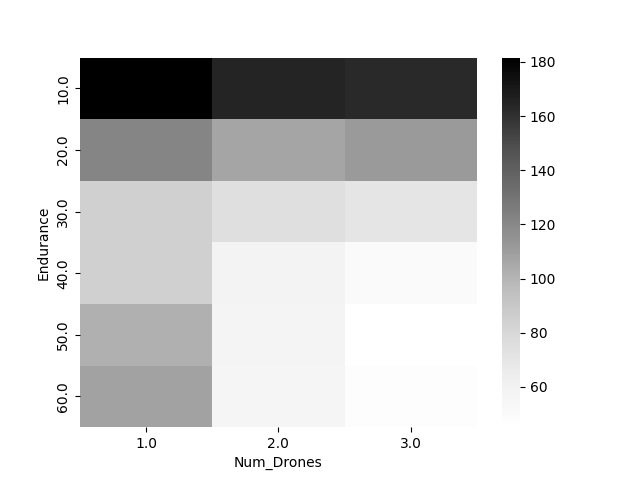
\includegraphics[width=\linewidth]{heatmap_gray.png}
\caption{Heatmap of objective function values depending on number of drones and drone capacities. The darker the color intensity the smaller the objective value. \label{fig:heatmap}}
\end{figure}
\noindent


\section{Case Study\label{section:CS}}

\noindent
In this section, we describe a realistic application of the system studied in this paper to perform surveillance operations. Considering the current COVID-19 restrictions, we focus on the problem of preventing and identifying possible concentrations of people during events such as popular or religious festivals. In particular, we consider the Courtyards Festival of Cordoba (\url{https://patios.cordoba.es/es/}). This is a social event that takes place every year in the city of Cordoba, Spain, during the first two weeks of May. Courtyard owners decorate their houses with many flowers trying to win the award that is offered by the \EN{Municipality}. During this competition, a festival runs in parallel with a number of artistic performances along six different paths located in different areas \EN{of} the city as shown in Figure \ref{fig:mapPF}.
In the pandemic context, to monitor the situation to avoid the concentration of people, we propose to apply a system consisting of one helicopter and a fleet of two drones.
This kind of system has been \EN{tested} successfully and has \EN{already been} applied in the military field by the US Army to leave the helicopter at the edge of dangerous airspace and release drones, which will then penetrate enemy territory and send back intelligence, surveillance and reconnaissance information (see \cite{FGA}).
In our application, the reason to adopt a similar system is the possibility \EN{of simultaneously inspecting} and in real time different paths, also reducing the risk of flying the helicopter over populated areas and the cost of moving the helicopter by minimizing the total length of its tour.

\begin{figure}[h!]
	\centering
	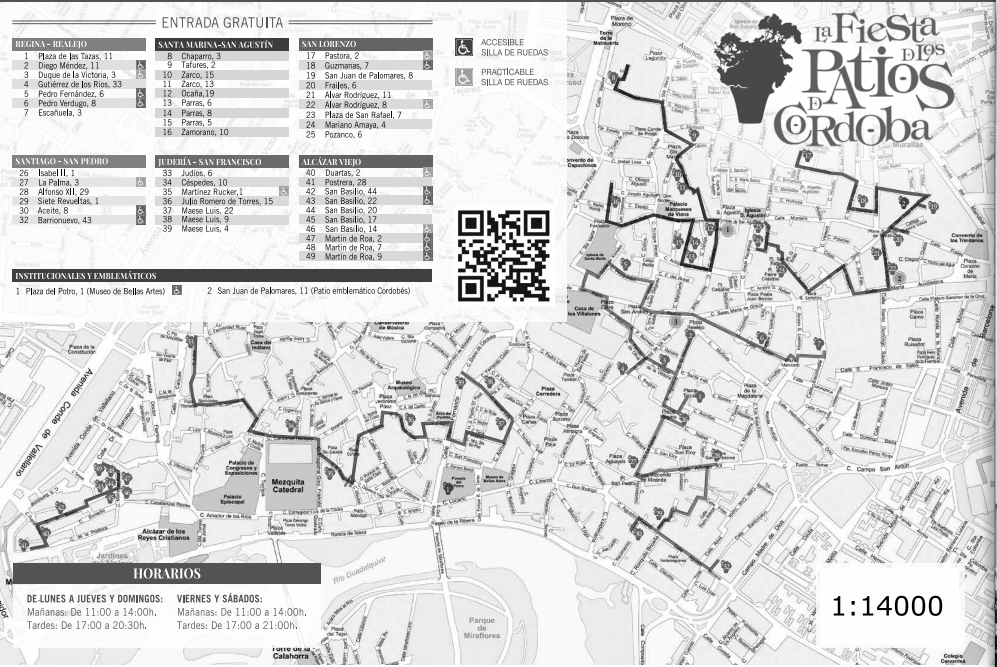
\includegraphics[width=0.6\linewidth]{first_gray.png}
	\caption{Map of the Courtyards Festival in Cordoba. \label{fig:mapPF}}
\end{figure}

\noindent
We run the models presented in Section \ref{Form} on this scenario starting from the initial solution provided by the matheuristic, where the 6 coloured paths reported in the map of Figure \ref{fig:mapPF} represent the 6 target graphs to be visited, in this case inspected, by the fleet of drones. In addition, we suppose that the drones' speed is 43 km/h while that of the helicopter is  30 km/h aiming to minimize costs.
Moreover, we assume that the fleet is composed \EN{of} two drones with an endurance equal to 7.5 minutes, and we impose that each target graph must be fully visited (inspected).  As we can see from Figure \ref{fig:Mtour_CO} and Figure \ref{fig:Mtour_PO}, the origin of the mothership tour coincides with the destination and it is located in an area of the city where it is possible to \EN{suppose} the take-off and landing of \EN{a} helicopter. Figure \ref{fig:Mtour_CO} reports the tour followed by the helicopter in the solution of the complete overlapping version of the problem, after 4 hours of running time. We can observe that the helicopter, starting from the origin, flies to the point $x_R^1$ that is the first rendezvous point, coinciding with the second launching point $x_L^2$. Then, it flies along the edge connecting $x_R^1$ with $x_R^2$, that is the second rendezvous point, which coincides with the third launching point $x_L^3$. Next, the helicopter flies to $x_R^3$ for retrieving the \EN{drone completing the third mission}. From the same point the fourth and last mission starts and ends at point $x_R^4$, that is also the final destination of the helicopter tour.\\
Figure \ref{fig:tourD_CO} shows the tour (gray dotted paths) followed by the two drones \EN{to inspect} the six paths. In particular, one drone, starts from the origin ($origin=x_L^1$) \EN{to visit} the path of "Alcazar Viejo". It is retrieved by the helicopter at point $x_R^1$ and from the same point both drones, are launched to visit respectively the paths of "Juderia-San Francisco" and "Santa Maria-San Agustin". Both drones end their mission at point $x_R^2$. From this latter point they are launched to perform the visits to the paths of "San Lorenzo" and "Regina-Realejo". Then, they are both retrieved by the  helicopter at point $x_R^3$ where only one drone starts its last mission to visit the path of "Santiago-San Pedro". In the meanwhile, the helicopter, containing the other drone, flies to point $x_R^4=dest$ where it retrieves the other and ends its tour.
The total time travelled by the helicopter is around 21 minutes.
We can observe that in the drone tour on \EN{the} "San Lorenzo" and "Regina-Realejo" graphs, there are two edges whose duplicate is represented with a dotted segment in Figure \ref{fig:tourD_CO}. They are associated with edges of the graph that are visited once, but traveled twice by the drone, in order to perform the inspection of the whole graph.\\
Figure \ref{fig:Mtour_PO} shows the mothership tour in the solution of the partial overlapping version of the problem, always obtained by setting a time limit of 4 hours. In this case, we can observe that the helicopter follows a different tour and that there are more launching and retrieving points due to the possibility of launching \EN{one} drone before retrieving the other. From Figure \ref{fig:tourD_PO} we can see that, differently from the complete overlapping version, both drones start their first mission from the origin $origin=x_L^1=x_L^2$. One drone visits the path of "Alcazar Viejo", while the other visits the path of "Santiago-San Pedro". The first is retrieved by the helicopter at point $x_R^3$ and is launched again from the point $x_L^4$. From this latter point this drone starts its second mission to visit the path of "Juderia-San Francisco". In the meantime, the helicopter flies to the point $x_R^5$ where the other drone is retrieved. From the same point $x_R^5=x_L^6$ this latter drone is then launched to inspect the path of "Santa Maria-San Agustin". Both drones are retrieved by the helicopter at the point $x_R^7=x_R^8$. From this latter point $x_R^8=x_L^9$ one drone is launched to visit the path of "Regina-Realejo". Then, the helicopter flies to the point $x_L^{10}$ from \EN{which} the other drone starts its last visit to the path of "San Lorenzo". Finally, the helicopter flies to the destination $dest$ and along its path, it retrieves the first drone at the point $x_R^{11}$ and then the other at the point $x_R^{12}$. Also in this case, \EN{as} in the solution of the complete overlapping version of the problem, we have one edge of the graph associated with the path of "Regina-Realejo" and one edge of the graph representing the path of "San Lorenzo", that are traversed twice represented with dotted segments in Figure \ref{fig:tourD_PO}. The total travel time of the helicopter is 19 minutes. It is slightly lower than \EN{that} associated with the solution of the complete overlapping version of the problem. Thus, even if on this scenario we cannot observe big changes in terms of the objective function value, we can see how the different assumptions associated with the two versions of the problem can influence the structure of the solution, by producing a different schedule of the drone missions and a different location of the launching and rendezvous points.\\
\noindent
All details of this case study, including map coordinates, .lp models and solutions can be found in \cite{Puerto2021}.


\begin{figure}[h!]
	\centering
	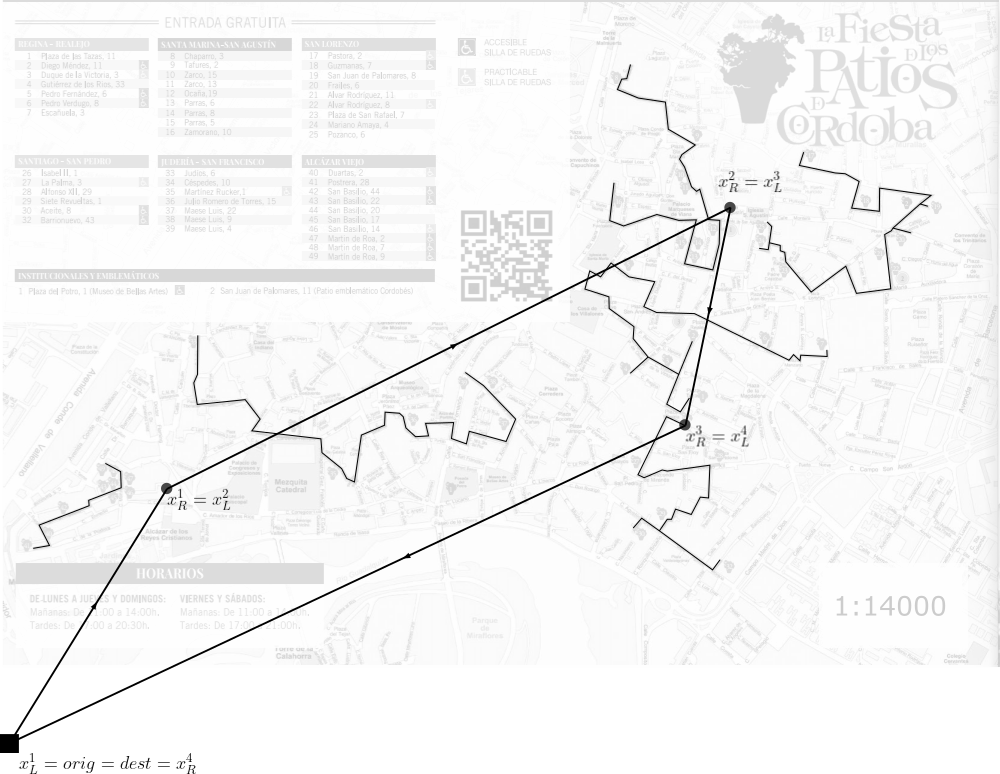
\includegraphics[width=0.6\linewidth]{synchronous_1_gray.png}
	\caption{Mothership tour (CO) \label{fig:Mtour_CO}}
\end{figure}
\begin{figure}[h!]
	\centering
	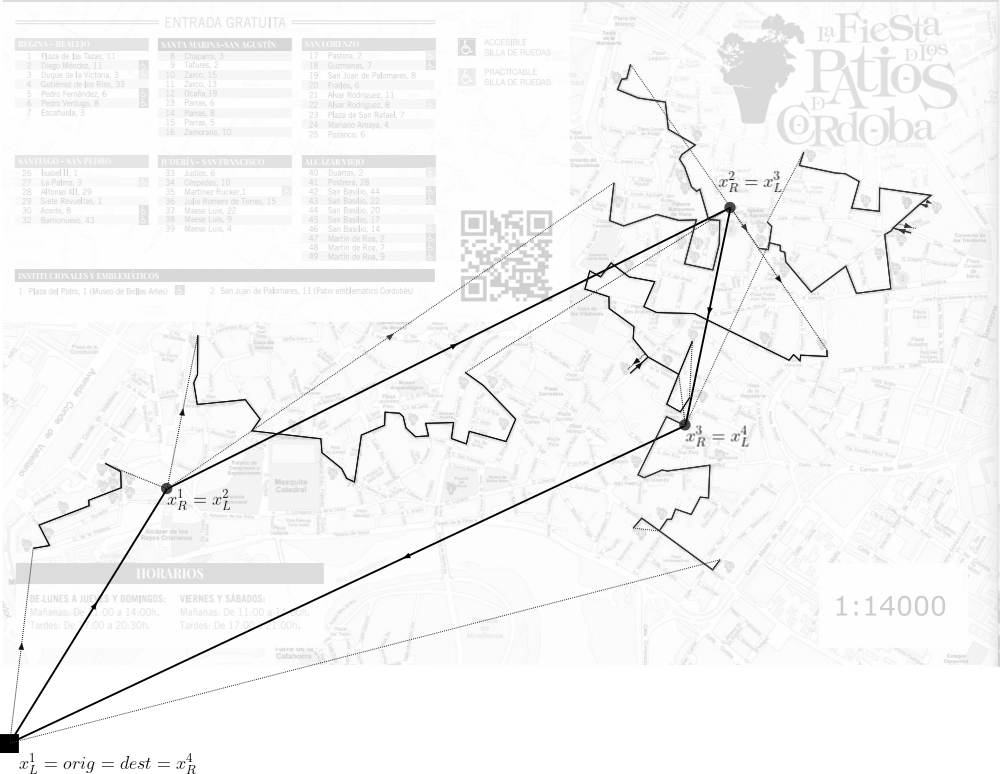
\includegraphics[width=0.6\linewidth]{synchronous_2_gray.png}
	\caption{The complete solution (CO) \label{fig:tourD_CO}}
\end{figure}

\begin{figure}[h!]
	\centering
	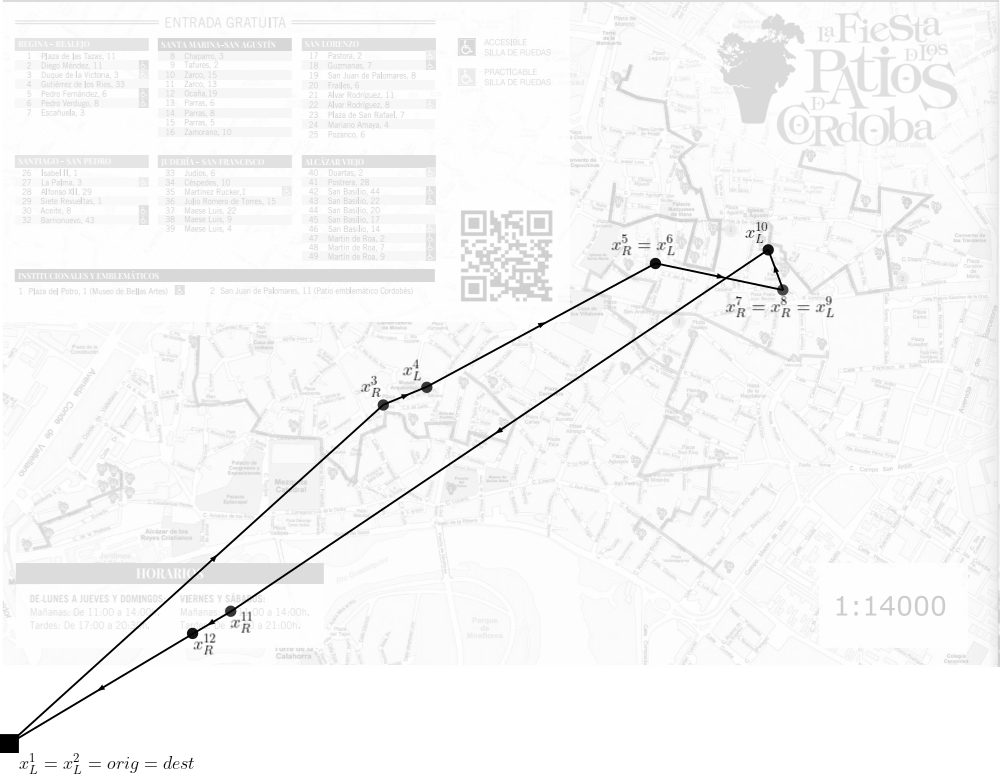
\includegraphics[width=0.6\linewidth]{asynchronous_1_gray.png}
	\caption{Mothership tour (PO) \label{fig:Mtour_PO}}
\end{figure}
\begin{figure}[h!]
	\centering
	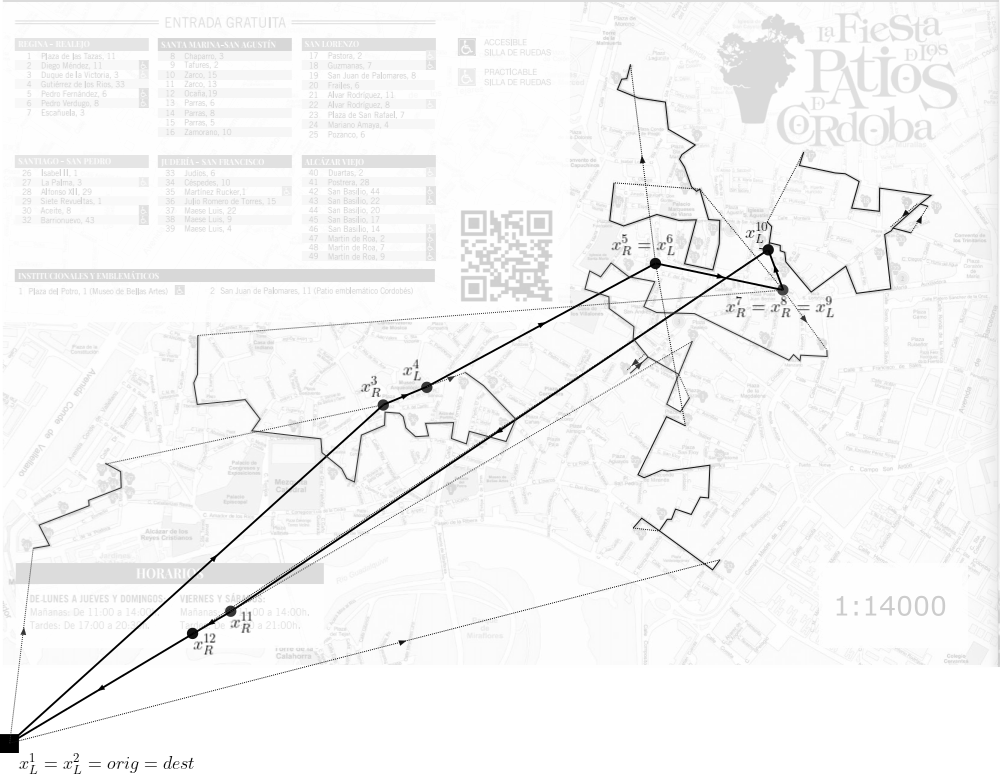
\includegraphics[width=0.6\linewidth]{asynchronous_2_gray.png}
	\caption{The complete solution (PO) \label{fig:tourD_PO}}
\end{figure}
\section{Concluding remarks\label{section:CR}}
\noindent
This paper has analyzed the coordination problem that arises between a mothership vehicle and a fleet of drones that must coordinate their routes to minimize the total time traveled by the mothership while visiting a set of targets modeled by graphs. We have presented exact mixed integer nonlinear programming formulations of the problem for its complete and partial overlapping versions. Moreover, we strengthen the models with some valid inequalities for them.\\
Our computational results show that the \EN{problem considered} is very challenging to solve even on small and medium size instances. For that reason, additionally, we have proposed a matheuristic algorithm that provides good quality feasible solutions in a short computing time; so that it is a good alternative to the exact method. We report extensive computational experiments on randomly generated instances. Moreover, we present a case study related to inspection activities in the context of COVID-19 restrictions. We show the application of the system described in this paper in the framework of the Courtyard\EN{s} Festival in the city of Cordoba, by illustrating the solution obtained by adopting the problem formulation, in both versions of the model, and its solution by means of the initialization provided by the proposed matheuristic.\\
\noindent
The formulation and algorithms proposed in this paper can be seen as a first building block to handle the coordination of systems composed \EN{of} a base vehicle and a number of  drones. Further research \EN{on} this topic must focus on finding faster and more accurate algorithms able to solve larger size instances. Moreover, it is also challenging to model more complex operations allowing \EN{drones to visit} more than one target per trip. Other extensions that may be considered can take into account that the time spent by the mothership to launch and retrieve the drones is not negligible as well as handling the speed of the mothership and drones as decision variables. These problems being very interesting are beyond the scope of the present paper and will be the focus of a follow up research line.
\section*{Acknowledgments}
This research has been partially supported by \EN{the} Spanish Ministry of Education and Science/FEDER grant number  PID2020-114594GB02, and projects Junta de Andalucia P18-FR-1422, FEDER-US-1256951, CEI-3-FQM331 and  \textit{NetmeetData}: Ayudas Fundaci\'on BBVA a equipos de investigaci\'on cient\'ifica 2019.



\bibliographystyle{elsarticle-num-names}


\bibliography{bibliography2.bib}
\section{Appendix}\label{App}
\noindent
In this section, we report an extension of the MINLP formulation presented in Section \ref{Form}, \EN{to deal} with the case of non\EN{-}homogeneous fleets of drones.
\noindent
In the following, we introduce the parameters or input data that formally describe the problem and that are summarized in Table \ref{table:At1}.
\noindent
The formulation in this appendix is \EN{quite} similar to the one in Section \ref{subsec:CO} but, because of the assumption of non\EN{-}homogeneous drones, it needs to keep track of the drones used in each action. This implies \EN{including} an extra index $\delta$ in most of the variables. For the sake of completeness, we have included the complete set of constraints of \EN{these} formulations although some of them are similar to those in Section \ref{subsec:CO}. Table \ref{table:At2} summarizes all the decision variables used in this formulation.

\begin{table}[!h]
	\scriptsize
	\centering
	\begin{tabular}{ | l | }
		\hline
		\textbf{Problem Parameters}\\
		\hline
		$origin$: coordinates of the point defining the origin of the mothership path (or tour).\\
		$dest$: coordinates of the point defining the destination of the mothership path (or tour).\\
		$\mathcal{G}$: set of the target graphs.\\
		$g = (V_g, E_g)$: set of nodes and edges of each target graph $g \in \mathcal{G}$.\\
		$\mathcal{L}(e_g)$: length of edge $e$ of graph $g \in \mathcal{G}$.\\
		$\mathcal{L}(g)=\sum_{e_g\in E_g} \mathcal L(e_g)$: total length of the graph $g\in\mathcal G$.\\
		$B^{e_g}, C^{e_g}$: coordinates of the endpoints of edge $e$ of graph $g \in \mathcal{G}$.\\
		$\alpha^{e_g}$: fraction of edge $e$ of graph $g \in \mathcal{G}$ that must be visited.\\
		$\alpha^{g}$: fraction of graph $g \in \mathcal{G}$ that must be visited.\\
		$v_M$: mothership speed.\\
		$\mathcal D$: set of drones.\\
		$v_\delta$: drone $\delta$ speed.\\
		$N_\delta$: drone $\delta$ endurance. \\
		$\mathcal{O}$: set of drone operations to perform visits to the target graphs\\
		$M$: big-M constant.\\
		\hline
	\end{tabular}
	\caption{Nomenclature for AMMDRPG with non-homogeneous fleet of drones}
	\label{table:At1}
\end{table}

\begin{table}[h!]
	\scriptsize
	\centering
	\begin{tabular}{|l|}
		\hline 
		\textbf{Binary and Integer Decision Variables}\\
		\hline
		$\mu^{e_g} \in \{0,1\}, \:\: \forall e_g \in E_g\:\: (g \in \mathcal{G})$: equal to 1 if edge $e$ of graph $g$ (or a fraction of it) is visited by the drone, 0 otherwise.\\
		$\text{entry}^{e_g} \in \{0,1\}, \:\: \forall e_g \in E_g\:\: (g \in \mathcal{G})$: auxiliary binary variable used for linearizing expressions.\\
		$u^{e_{g}o\delta} \in \{0,1\}, \:\: \forall e_g \in E_g\:\: (g \in \mathcal{G}), \:\:\forall o \in \mathcal O, \:\: \forall \delta \in \mathcal D$: equal to 1 if the drone $\delta$ enters in graph $g$ by the edge $e_g$ at operation $o$,\\ \hspace*{1cm} 0 otherwise.\\
		$z^{e_{g}e^{'}_{g}} \in \{0,1\}, \:\: \forall e_g, e_g' \in E_g\:\: (g \in \mathcal{G})$: equal to 1 if the drone goes from $e_g$ to $e^{'}_{g}$, 0 otherwise.\\
		$v^{e_{g}o\delta} \in \{0,1\}, \:\: \forall e_g \in E_g\:\: (g \in \mathcal{G}), \:\: \forall o \in \mathcal O, \:\: \forall \delta \in \mathcal D$: equal to 1 if the drone $\delta$ exits from graph $g$ by $e_g$ at operation $o$,\\ \hspace*{1cm} 0 otherwise.\\
		\hline
		\textbf{Continuous Decision Variables}\\
		\hline
		$s^{e_g}\in[0, |E_g|-1],\:\: \forall e_g \in E_g\:\: (g \in \mathcal{G})$: continuous non negative variable representing the order of visit \EN{to} the edge $e$ of graph $g$.\\
		$\rho^{e_g} \in [0,1]$ and $\lambda^{e_g} \in [0,1], \:\: \forall e_g \in E_g\:\: (g \in \mathcal{G})$: defining the entry and exit points on $e_g$.\\
		$\nu_\text{min}^{e_g}$ and $\nu_\text{max}^{e_g} \in [0,1], \:\: \forall e_g \in E_g\:\: (g \in \mathcal{G})$: auxiliary variables used for linearizing expressions.\\
		$p^{e_g}\in [0, 1], \:\: \forall e_g \in E_g\:\: (g \in \mathcal G)$: auxiliary variable used for modeling the product of $\mu^{e_g}$ and $|\lambda^{e_g}-\rho^{e_g}|$.\\
		$x_L^o\in\mathbb R^2, \:\: \forall o \in \mathcal O$: coordinates representing the point where the mothership launches the drones at operation $o$.\\
		$x_R^o\in\mathbb R^2, \:\: \forall o \in \mathcal O$: coordinates representing the point where the mothership retrieves the drones at operation $o$.\\
		$R^{e_g}\in\mathbb R^2, \:\: \forall e_g \in E_g\:\: (g \in \mathcal{G})$: coordinates representing the entry point on edge $e_g$ of graph $g$.\\
		$L^{e_g}\in\mathbb R^2, \:\: \forall e_g \in E_g\:\: (g \in \mathcal{G})$: coordinates representing the exit point on edge $e_g$ of graph $g$.\\
		$d_L^{e_go\delta} \geq 0, \:\: \forall e_g \in E_g\:\: (g \in \mathcal{G}),\:\: \forall o \in \mathcal O, \:\: \forall \delta\in\mathcal D$: representing the distance traveled by the drone $\delta$ from the launching\\
		\hspace*{1cm} point $x_L^o$ on the mothership at operation $o$ to the first visiting point $R^{e_g}$ on $e_g$.\\
		$p_L^{e_go\delta} \geq 0, \:\: \forall e_g \in E_g\:\: (g \in \mathcal{G}), \:\:\forall o \in \mathcal O, \:\:\forall \delta\in\mathcal D$: auxiliary variable used for modeling the product of $d_L^{e_go\delta}$ and $u^{e_go\delta}$.\\
		$d^{e_g} \geq 0, \:\: \forall e_g \in E_g \:\: (g \in \mathcal{G})$: representing the distance traveled by the drone from the rendezvous point $R^{e_g}$ to the \\
		\hspace*{1cm} launching point $L^{e_g}$ on $e_g$. \\
		$d^{e_ge^\prime_g} \geq 0, \:\: \forall e_g, e^\prime_g \in E_g \:\: (g \in \mathcal{G})$: representing the distance traveled by the drone from the launching point $L^{e_g}$ on $e_g$ to\\
		\hspace*{1cm}  the rendezvous point $R^{e^\prime_g}$ on $e^\prime_g$.\\
		$p^{e_ge^\prime_g} \geq 0, \:\: \forall e_g, e^\prime_g \in E_g \:\: (g \in \mathcal{G})$: auxiliary variable used for modeling the product of $d^{e_ge^\prime_g}$ and $z^{e_ge^\prime_g}$.\\
		$d_R^{e_go\delta} \geq 0, \:\: \forall e_g \in E_g\:\: (g \in \mathcal{G}), \:\: \forall o \in \mathcal O, \:\:\forall \delta\in\mathcal D$: representing the distance traveled by the drone $\delta$ from the last visiting point\\
		\hspace*{1cm} $L^{e_g}$ on $e_g$ to the rendezvous point $x_R^o$ on the mothership at operation $o$.\\
		$p_R^{e_go\delta} \geq 0, \:\: \forall e_g \in E_g\:\: (g \in \mathcal{G}), \:\:\forall o \in \mathcal O, \:\:\forall \delta\in\mathcal D$: auxiliary variable used for modeling the product of $d_R^{e_go\delta}$ and $v^{e_go\delta}$.\\
		$d_{origin}\geq 0$: distance from the origin $origin$ to the first launching point $x_L^1$.\\
		$d_{LR}^o \geq 0, \:\: \forall o \in \mathcal O$: representing the distance traveled by the mothership from the launching point $x_L^o$ to the rendezvous\\
		\hspace*{1cm}   point $x_R^o$ at operation $o$.\\
		$d_{RL}^o \geq 0, \:\: \forall o \in \mathcal O\setminus|\mathcal O|$: representing the distance traveled by the mothership from the rendezvous point $x_R^o$ at operation $o$ to the \\ 
		\hspace*{1cm}  launching point $x_L^{(o+1)}$ at operation $o+1$.\\
		$d_{dest}\geq 0$: distance from the last retrieving point $x_R^{|\mathcal O|}$ to the destination $dest$.\\
		$time_D^o \geq 0, \:\: \forall o \in \mathcal O$: maximum time spent by a drone during operation $o$.\\
		$time_M^o \geq 0, \:\: \forall o \in \mathcal O$: time spent by the mothership to go from the launching point $x_L^o$ to the retrieving point $x_R^o$ of operation $o$.\\
		$time_M \geq 0$: total time spent by the mothership to go from the origin to the destination.\\
		\hline
	\end{tabular}
	\caption{Decision Variables for AMMDRPG with non-homogeneous fleet of drones}
	\label{table:At2}
\end{table}

\subsection*{Visits \EN{to} graphs}
\noindent
As for the case of a homogeneous fleet of drones presented in Section \ref{Form}, to represent the movement of the drone within a graph $g\in\mathcal G$, we proceed to introduce some notation\EN{s} related to $g$.
Let $g = (V_g, E_g)$ be a graph in $\mathcal G$ whose total length is denoted by $\mathcal L(g)$. Here, $V_g$ denotes the set of nodes and $E_g$ denotes the set of edges connecting pairs of nodes.  Let $e_g$ be the edge $e$ of the graph $g \in G$ and let $\mathcal  L(e_g)$ be its length. Each edge $e_g$ is parameterized by its endpoints $B^{e_g}= (B^{e_g}(x_1), B^{e_g}(x_2))$ and $C^{e_g}= (C^{e_g}(x_1), C^{e_g}(x_2))$ and we can compute its length $\mathcal L(e_g) =\|C^{e_g} -  B^{e_g}\|$. 
\noindent
For each edge $e_g$ an indicator binary variable $\mu^{e_g}$ \EN{is associated} that is one if the drone visits the segment $e_g$. Moreover, we define the entry and exit points $R^{e_g}=(B^{e_g},C^{e_g},\rho^{e_g})$ and $L^{e_g}=(B^{e_g},C^{e_g},\lambda^{e_g})$ that determine the fraction of the edge visited by the drone. The coordinates of the points $R^{e_g}$ and $L^{e_g}$ are given, respectively by 
$$R^{e_g} = \rho^{e_g} B^{e_g} + (1- \rho^{e_g})C^{e_g} \quad\text{ and }\quad L^{e_g} = \lambda^{e_g} B^{e_g} + (1- \lambda^{e_g})C^{e_g},$$ where $\rho^{e_g} \in [0,1]$ and $\lambda^{e_g} \in [0,1]$ are variables to determine the position of the points on the segment.

\noindent
As discussed in Section \ref{section:desc}, we consider two modes of visit to the target graphs $g\in \mathcal{G}$:
\begin{itemize}
	\item Visiting a fraction $\alpha^{e_g}$ of each edge $e_g$ which can be modeled by using the following constraints:
	\begin{equation}\label{eq:NOalphaE}\tag{$\alpha$-E}
		|\lambda^{e_g} - \rho^{e_g}|\geq \alpha^{e_g}, \quad \forall e_g\in E_g.
	\end{equation}
	These inequalities state that the difference between the parametrizations of the entry and exit points associated \EN{with} each edge $e_g$ must be higher than the fraction of the length of $e_g$ required to be traversed.
	\item Visiting a fraction $\alpha^g$ of the total length of the graph:
	\begin{equation}\label{eq:NOalphaG}\tag{$\alpha$-G}
		\sum_{e_g\in E_g} \mu^{e_g}|\lambda^{e_g} - \rho^{e_g}|\mathcal L(e_g) \geq \alpha^g\mathcal L(g).
	\end{equation}
	\noindent
	This constraint ensures that the sum of the fractions of the length of those edges chosen to be crossed must be higher than the fraction of the length of $g$ required to be traversed.
\end{itemize}



\bigskip
\noindent
In both cases, the corresponding constraints are nonlinear. To linearize them, we need to introduce a binary variable $\text{entry}^{e_g}$ that determines the traveling direction on the edge $e_g$ as well as the definition of the auxiliary variables $\nu_\text{min}^{e_g}$ and $\nu_\text{max}^{e_g}$ of the access and exit points on that segment. Then, for each edge $e_g$, the absolute value constraint \eqref{eq:NOalphaE} can be represented by:


\begin{equation}\label{eq:NOalpha-E}\tag{$\alpha$-E}
	|\rho^{e_g}-\lambda^{e_g}|\geq \alpha^{e_g} \Longleftrightarrow
	\left\{
	\begin{array}{ccl}
		\rho^{e_g} - \lambda^{e_g}                       & =    & \nu_\text{max}^{e_g} - \nu_\text{min}^{e_g},                                     \\
		\nu_\text{max}^{e_g}                         & \leq & 1-{\text{entry}^{e_g}},                                   \\
		\nu_\text{min}^{e_g}                      & \leq & {  \text{entry}^{e_g}},                                        \\
		\nu_\text{min}^{e_g}, \,\nu_\text{max}^{e_g} & \geq & 0, \\
		
		\nu_\text{max}^{e_g} + \nu_\text{min}^{e_g} & \geq & \alpha^{e_g}.
		\\
	\end{array}
	\right.
\end{equation}

\noindent
The first four inequalities model the standard trick of the linearization of the absolute value. The last constraint ensures that the value of the linear expression of the absolute value is higher than the required fraction $\alpha^{e_g}$.
\noindent
Similarly, \eqref{eq:NOalphaG} can be linearized as follows:
\begin{equation}\label{eq:NOalpha-G}\tag{$\alpha$-G}
	\sum_{e_g\in E_g} \mu^{e_g}|\rho^{e_g}-\lambda^{e_g}|\mathcal L(e_g)\geq \alpha^g\mathcal L(g). \Longleftrightarrow
	\left\{
	\begin{array}{ccl}
		\rho^{e_g} - \lambda^{e_g}                       & =    & \nu_\text{max}^{e_g} - \nu_\text{min}^{e_g},                                     \\
		\nu_\text{max}^{e_g}                         & \leq & 1-{\text{entry}^{e_g}},                                   \\
		\nu_\text{min}^{e_g}                      & \leq & {  \text{entry}^{e_g}},                                        \\
		\nu_\text{min}^{e_g}, \,\nu_\text{max}^{e_g} & \geq & 0, \\
		p^{e_g} & \leq & \nu_\text{max}^{e_g} + \nu_\text{min}^{e_g}, \\
		p^{e_g} & \leq & \mu^{e_g}, \\
		p^{e_g} & \geq & \nu_\text{max}^{e_g} + \nu_\text{min}^{e_g} + \mu^{e_g} - 1, \\
		\sum_{e_g\in E_g} p^{e_g}\mathcal L(e_g) & \geq & \alpha^{g}\mathcal L(g),
		\\
	\end{array}
	\right.
\end{equation}
where $p^{e_g}$ is the auxiliary variable that represents the product of the binary variable $\mu^{e_g}$ and the absolute value difference $|\rho^{e_g} - \lambda^{e_g}|$. The first four inequalities \EN{again linearize} the absolute value expression. The (second) following three constraints model the product of the expression of the absolute value and the binary variable $\mu^{e_g}$. The last inequality ensures that the fraction of the length of those edges chosen to be crossed must be higher than the fraction of the length of $g$ required to be traversed.

\subsection*{Elimination of subtours}
\noindent
As already presented in Section \ref{Form},  to prevent the existence of subtours within each graph $g\in \mathcal G$ that the drone must visit, one can include, among others, either the compact formulation that uses the Miller-Tucker-Zemlin constraints (MTZ) or the subtour elimination constraints (SEC).\\
\noindent
For the MTZ formulation, we use the continuous variables $s^{e_g}$, defined in Table \ref{table:At2}, that state the order to visit the edge $e_g$ and set the following constraints for each $g\in\mathcal G$:

\begin{align}
	s^{e_g} - s^{e^\prime_g} + |E_g|z^{e_ge^\prime_g} & \leq |E_g| - 1  , &\quad\forall e_g \neq e_g'\in E_g, \tag{MTZ$_1$} \label{NOMTZ1}\\
	0 & \leq s^{e_g} \leq |E_g| - 1, &\quad\forall e_g\in E_g.\tag{MTZ$_2$}\label{NOMTZ2}
\end{align}

\noindent
Alternatively, we can also use the family of subtour elimination constraints for each $g\in\mathcal G$:
\begin{equation}\tag{SEC}\label{NOSEC}
	\sum_{e_g, e^\prime_g \in S} z_g^{e_ge^\prime_g} \leq |S| - 1, \quad \forall S\subset E_g.
\end{equation}

\noindent
To find SEC inequalities, as usual, we search for disconnected components in the current solution. Among them, we choose the shortest subtour found in the solution to be added as a lazy constraint to the model.\\

\subsection*{Drone constraints}
\noindent
To model this problem, as already described in Section \ref{subsec:CO}, we adopt the concept of operation.
Let us denote by $\mathcal O$ the set of operations that the mothership and the fleet of drones have to carry out. These operations are visits to the different graphs in $\mathcal G$ with the required constraints. An operation $o\in\mathcal O$ is referred to as the event in which the mothership launches some drones from a taking-off location, denoted by $x_L^o$ and later it takes them back \EN{to} a rendezvous location $x_R^o$. 

\noindent
For each operation $o\in\mathcal O$, each of the drones launched from the mothership must follow a path starting from and returning to the mothership, while visiting the required edges of $g$.





\noindent
To include the definition of these paths in our mathematical programming formulation, we need to make decisions to choose:
\begin{itemize}
	\item The optimal assignment of drones \EN{to visit} graphs in a given operation $o$.
	\item The order to visit the edges of each graph in its corresponding operation.
\end{itemize}

\noindent
We model the route that the drone follows by using the binary variables $u^{e_go\delta}$, $z^{e_ge^\prime_g}$ and $v^{e_go\delta}$ defined in Table \ref{table:At2}.

\begin{align}
	\sum_{g\in \mathcal G}\sum_{e_g\in E_g}  u^{e_go\delta} & \leq 1, &\forall o\in \mathcal O, \forall \delta\in\mathcal D.\label{st:NODEnt}\\
	\sum_{g\in \mathcal G}\sum_{e_g\in E_g}  v^{e_go\delta} & \leq 1, &\forall o\in \mathcal O, \forall \delta\in\mathcal D.\label{st:NODExt} \\
	\sum_{e_g\in E_g} \sum_{o\in \mathcal O} \sum_{\delta\in\mathcal D} u^{e_go\delta} & = 1, &\forall g\in\mathcal G, \label{st:NODEng}\\%\tag{D
		\sum_{e_g\in E_g} \sum_{o\in \mathcal O} \sum_{\delta\in\mathcal D} v^{e_go\delta} & = 1, &\forall g\in\mathcal G, \label{st:NODExg}\\%\tag{D
			\sum_{e_g\in E_g} u^{e_go\delta} & = \sum_{e_g\in E_g} v^{e_go\delta}, &\forall g\in\mathcal G, \forall o\in \mathcal O, \forall \delta\in\mathcal D, \label{st:NODuv}\\%\tag{D
				\sum_{o\in \mathcal O} \sum_{\delta \in \mathcal D} u^{e_go\delta} + \sum_{e^\prime_g\in E_g} z_g^{e^\prime_ge_g} & = \mu^{e_g}, &\forall e_g\in E_g:g\in\mathcal G, \label{st:NODInu}\\
				\sum_{o\in \mathcal O} \sum_{\delta \in \mathcal D} v^{e_go\delta} + \sum_{e^\prime_g\in E_g} z_g^{e_ge^\prime_g} & = \mu^{e_g}, &\forall e_g\in E_g:g\in\mathcal G. \label{st:NODInv}
			\end{align}
			
			\noindent 
			Inequalities \eqref{st:NODEnt} and \eqref{st:NODExt} state that a drone $\delta$ visits at most one graph $g$ at operation $o$.  Constraints \eqref{st:NODEng} and \eqref{st:NODExg} \EN{ensure} that each graph is visited at some operation $o$ by some drone $\delta$. Equations \eqref{st:NODuv} ensure that the operation of entering and exiting the graph $g$ occurs in the same operation $o$ and is done by the same drone $\delta$. Constraints \eqref{st:NODInu} state that if an edge $e$ of graph $g$ is visited by the drone $\delta$, one of two alternative situations must occur: either $e$ is the first edge of graph $g$ visited by the drone $\delta$ at operation $o$, or edge $e$ is visited by the drone $\delta$ after visiting another edge $e^\prime$ of graph $g$. Similarly, constraints \eqref{st:NODInv} state that if an edge $e$ of graph $g$ is visited by the drone $\delta$, either $e$ is the last edge of graph $g$ visited by the drone at operation $o$, or the drone $\delta$ must move to another edge $e^\prime$ of graph $g$ after visiting edge $e$.
			
			\subsubsection*{Distance and Time Constraints}
			\noindent
			The goal of the \AMD\xspace (specify) is to find a feasible solution that minimizes the total time traveled by the mothership. To account for the different distances between the decision variables of the model, we need to set the continuous variables $d_L^{e_go\delta}$, $d^{e_g}$, $d^{e_ge^\prime_g}$, $d_R^{e_go\delta}$, $d_{origin}$, $d_{RL}^o$, $d_{LR}^o$ and $d_{dest}$ defined in Table \ref{table:At2}. This can be done by means of the following constraints:
			
			
			\begin{align*}
				\|x_L^o- R^{e_g}\| & \leq  d_L^{e_go\delta},  &\quad \forall e_g\in E_g:g\in \mathcal{G}, \forall o\in \mathcal O, \forall \delta\in\mathcal D, \tag{DIST$_{1}$-o} \label{eq:NOd1}\\
				\|R^{e_g}- L^{e_g}\| & \leq  d^{e_g},  &\quad \forall e_g\in E_g:g\in \mathcal{G}, \tag{DIST$_{2}$-o} \label{eq:NOd2}\\
				\|R^{e_g}- L^{e^\prime_g}\| & \leq  d^{e_ge^\prime_g}, &\quad \forall e_g\neq e_g'\in E_g:g\in \mathcal{G}, \tag{DIST$_{3}$-o} \label{eq:NOd3}\\
				\|L^{e_g}- x_R^o\| & \leq  d_R^{e_go\delta}, &\quad \forall e_g:g\in \mathcal{G},\forall o\in \mathcal O, \forall \delta\in\mathcal D, \tag{DIST$_{4}$-o} \label{eq:NOd4}\\
				\|origin - x_L^1\| & \leq d_{origin}, \tag{DIST$_5$-o}\label{eq:NOd5}\\
				\|x_L^o- x_R^o\| & \leq  d_{LR}^o, & \quad \forall o\in \mathcal O. \tag{DIST$_{6}$-o} \label{eq:NOd6}\\
				\|x_R^o- x_L^{o+1}\| & \leq  d_{RL}^o, & \quad \forall o\in \mathcal O:o<|\mathcal O|, \tag{DIST$_{7}$-o} \label{eq:NOd7}\\
				\|x_R^{|\mathcal O|} - dest\| & \leq d_{dest}, \tag{DIST$_8$-o}\label{eq:NOd8}\\
			\end{align*}
			
			\noindent
			Thus, we can express the time spent by a drone $\delta \in \mathcal D$ to visit a graph $g \in \mathcal G$ during operation $o \in \mathcal O$ as follows:
			
			\begin{equation}
				time_\delta^o \geq \frac{1}{v_\delta}\left(\sum_{e_g\in E_g} u^{e_go\delta}d_L^{e_go\delta} + \sum_{e_g, e^\prime_g\in E_g}z^{e_ge^\prime_g}d^{e_ge^\prime_g} + \sum_{e_g\in E_g} \mu^{e_g}d^{e_g} + \sum_{e_g\in E_g} v^{e_go\delta}d_R^{e_go\delta}\right) - N_\delta(1 - \sum_{e_g\in E_g} u^{e_go\delta})
				\label{eq:NOtimed}
			\end{equation}
			
			\noindent
			The first addend within the brackets in the RHS of constraint (\ref{eq:NOtimed}), accounts for the time spent by drone $\delta$ to (depart) go from the launching point $x_L^o$ to the first retrieving point in the graph $R^{e_g}$. The second addend considers the time consumed by the drone to go from edge $e_g$ to $e_g'$ in the graph $g$. The third computes the time required for traversing the required edges in $g$. The fourth measures the time to travel from the last launching point $L^{e_g''}$ to the retrieving point $x_R^o$.
			The bigM term ensures that the constraint becomes active only when a graph $g$ is visited during operation $o$ by drone $\delta$. The reader may observe that the endurance constraint \eqref{NOCAP} restricts the time spent by the drone to perform the operation $o$ to be less than its endurance $N_\delta$. Hence, it is possible to take $N_\delta$ as a bigM constant in \eqref{eq:NOtimed}.\\
			
			
			\noindent
			In order to compute the maximum time spent by a drone to visit a graph $g \in \mathcal G$ associated with operation $o \:\:\ \forall o \in \mathcal O$, we introduce the following constraints:
			
			\begin{equation}
				time_D^o \geq time_\delta^o \:\: \forall \delta \in \mathcal D
				\label{eq:NOtimeD}
			\end{equation}
			
			\noindent
			Constraints (\ref{eq:NOtimeMO}) defines the time spent by the mothership to go from the launching point $x_L^o$ to the retrieving point $x_R^o$ associated with operation $o$. 
			
			\begin{equation}
				time_M^o = \frac{d_{LR}^o}{v_M} \:\: \forall o \in \mathcal O
				\label{eq:NOtimeMO}
			\end{equation}
			
			\noindent
			Thus, the overall time spent by the mothership to move from the origin to the destination can be expressed as follows:
			
			\begin{equation}
				time_M = \frac{1}{v_M} (d_{origin} + \sum_{o \in \mathcal O} (d_{LR}^o + d_{RL}^o) + d_{dest})
				\label{eq:NOtimeM}
			\end{equation}
			
			
			\subsubsection*{Coordination and Endurance Constraints}
			\noindent
			The coordination between the drones and the mothership must ensure that the maximum time $time_D^o$ spent by a drone to visit a graph $g$ at operation $o$ is less than or equal to the time that the mothership needs to move from the launching point to the retrieving point during operation $o$. To this end, we need to define the following coordination constraint for each operation $o\in \mathcal O$:
			
			\begin{equation}\tag{DCW-CO}\label{NODCW}
				time_D^o \leq time_M^o
			\end{equation}
			
			
			
			\noindent
			We can model the time endurance constraint for a particular operation $o\in \mathcal O$ and drone $\delta \in \mathcal D$ by limiting the time traveled by the drone $\delta$ for this operation $o$:
			
			\begin{equation}\tag{Endurance-CO}\label{NOCAP}
				time_\delta^o \leq N_\delta.
			\end{equation}
			
			
			
			
					
			
			\subsubsection*{AMMDRPG-Complete Overlapping Formulation (with non\EN{-}homogeneous fleet of drones)}
			\noindent
			Putting together all the constraints introduced before, the following formulation minimizes the total time traveled by the mothership, ensuring the coordination with the fleet of drones while guaranteeing the required coverage of the target graphs. 
			\begin{mini*}|s|
				{}{time_M}{}{} \label{NOAMMDRPG} \tag{AMMDRPG-Complete Overlapping with \EN{a} non-homogeneous fleet of drones}
				\addConstraint{\eqref{NOMTZ1}-\eqref{NOMTZ2}} \text{ or }  \eqref{NOSEC}
				\addConstraint{\eqref{eq:NOalpha-E} \text{ or } \eqref{eq:NOalpha-G}}{}{}
				\addConstraint{\eqref{st:NODEnt}-\eqref{st:NODInv}}{}{}
				\addConstraint{\eqref{eq:NOtimed}-\eqref{eq:NOtimeM}}{}{}
				\addConstraint{\eqref{eq:NOd1}-\eqref{eq:NOd8}}{}{}
				\addConstraint{\eqref{NODCW}}{}{}
				\addConstraint{\eqref{NOCAP}}{}{}
			\end{mini*}
			
			\noindent
			The objective function accounts for the time traveled by the mothership. Constraints \eqref{st:NODEnt}-\eqref{st:NODInv} model the route followed by the drone $\delta\in\mathcal D$, \eqref{NOMTZ1} - \eqref{NOMTZ2} \text{ or } \eqref{NOSEC} ensure that the displacement of the drone $\delta\in\mathcal D$ assigned to the target graph $g\in\mathcal G$ is a route, \eqref{eq:NOalpha-E} \text{ or } \eqref{eq:NOalpha-G} define what is required in each visit to a target graph. Finally, constraints (\ref{eq:NOd1})-(\ref{eq:NOd8}) set the variables $d_L^{e_go\delta}$, $d^{e_g}$, $d^{e_ge^\prime_g}$, $d_R^{e_go\delta}$, $d_{origin}$, $d_{RL}^o$, $d_{LR}^o$ and $d_{dest}$, defined in Table \ref{table:At2}, which represent Euclidean distances needed in the model. \\
			
			\subsection*{Strengthening the formulations}
			\noindent
			In this section\RE{,} we present some results that adjust the bigM constants for each of the models. These constants appear when we linearize the bilinear terms of \eqref{eq:NOtimed}. We use the McCormick's envelopes \EN{again} by adding variables $p\geq 0$  representing the products. \CV{To} strengthen the formulations\RE{,} we provide tight upper and lower bounds for those constants. The reader may note that the same bounds can be used for both models. Therefore, wlog, we focus on the bigM constants that appear in (\ref{NOAMMDRPG}).
			
						
			
			
			\subsubsection*{Big $M$ constants bounding the distance from the launching / rendezvous point on the path followed by the mothership to the rendezvous / launching point on the target graph $g\in \mathcal{G}$}
			
			
				\noindent
				\RE{To linearize the first addend in \eqref{DCW}}, we define the auxiliar\CV{y} non-negative continuous variables $p_L^{e_go\delta}$ (resp. $p_R^{e_go\delta}$) and we model the product by including the following constraints:
				\begin{align*}
					\RE{p_L^{e_go\delta}} & \RE{\leq  M_L^{e_go\delta}u^{e_go\delta},}\\
					\RE{p_L^{e_go\delta}} & \RE{\leq d_L^{e_go\delta},} \\
					p_L^{e_go\delta} & \geq m_L^{e_go\delta} u^{e_go\delta}, \\
					p_L^{e_go\delta} & \geq d_L^{e_go\delta} - M_L^{e_go\delta}(1-u^{e_go\delta}).
				\end{align*}
				\RE{Note that, among all graph nodes and the origin and destination points, it is possible to identify the pair of points at the maximum distance. From this pair of points, we can build a circle whose diameter is the segment joining them. Hence, because we are minimizing the distance traveled by the mothership, every launching  or rendezvous point is inside this circle and the best upper bound $M_L^{e_go\delta}$ or $M_R^{e_go\delta}$ can be described as:}
				
				$$
				M_R^{e_go\delta} = \max_{\{v\in V_g\cup\{\text{origin}, \text{dest}\}, v'\in V_{g'}\cup\{\text{origin}, \text{dest}\} : g, g'\in\mathcal G\}} \|v - v'\| = M_L^{e_go\delta}.
				$$
				
				\noindent
				On the other hand, the minimum distance in this case can be zero. This bound is attainable whenever the launching or rendezvous points of the mothership are the same \EN{as} the rendezvous or launching point on the target graph $g\in \mathcal{G}$.
				
		
			
			
			\subsubsection*{Bounds on the big$M$ constants for the distance from the launching to the rendezvous points on the target graph $g\in \mathcal{G}$.} 
			\noindent
			When the drone visits a graph $g$, it has to go from one edge $e_g$ to another edge $e'_g$ depending on the order given by $z^{e_ge_g'}$. This fact produces a product of variables linearized by the following constraints:
			\begin{align*}
				p^{e_ge'_g} & \leq M^{e_ge_g'} z^{e_ge_g'}, \\
				p^{e_ge'_g} & \leq d^{e_ge_g'}, \\
				p^{e_ge'_g} & \geq m^{e_ge_g'} d^{e_ge_g'}, \\
				p^{e_ge_g'} & \geq d^{e_ge_g'} - M^{e_ge_g'}(1-z^{e_ge_g'}).
			\end{align*}
			
			\noindent
			Since we are taking into account the distance between two edges $e\RE{_g}=(B^{e_g},C^{e_g}), \, e\RE{_g}'=(B^{e^\prime_g},C^{e^\prime_g})\in E_g$, the maximum distance between their vertices gives us the upper bound:
			\begin{align*}
				M^{e_g e^\prime_g} = & \max\{\|B^{e_g} - C^{e^\prime_g}\|, \|B^{e_g} - B^{e^\prime_g}\|, \|C^{e_g} - B^{e^\prime_g}\|, \|C^{e_g} - C^{\RE{e'_g}}\|\}. 
			\end{align*}
			We observe that the minimum distance between edges $m^{e_g e^\prime_g}$ can \EN{easily be} obtained computing the minimum distance between two edges, which results in a simple second-order cone program.
			
		
			
			
			\subsection*{Experimental results}
			\noindent
			In this section we discuss the results obtained testing the formulation of the \AMD\xspace with a non\EN{-}homogeneous fleet of drones, presented in Appendix \ref{App}, on the same set of instances described in Section \ref{section:results}.\\
			\noindent
			Table \ref{table:tab2} reports the results obtained by adopting the commercial solver Gurobi. We consider the exact solution both providing and not providing an initial solution computed by the matheuristic described in Section \ref{Math}. More precisely, the first column of Table \ref{table:apptab2} indicates the number of target graphs to be visited by the fleet of drones, the second column reports the endurance of the drones, the third column distinguishes between the visit of a fraction of each edge (e) and a fraction of each target graph (g). The fourth column reports the size of the fleet of drones. This last column contains three subcolumns reporting, for each cardinality of the set $\mathcal D$, respectively, the average percentage gap without initialization (wi), the average percentage gap with initialization of the solution provided by the matheuristic (i) and the solution time, in seconds, of the matheuristic (TimeH) for each combination of the listed parameters. The time limit of these experiments is set equal to 2 hours.\\
			We can observe that the value of the average percentage gap ranges between a minimum of 66.9\% and a maximum of 97.43\%. This shows that the model is hard to \EN{solve} even with small size instances. Moreover, we can see that in most of the cases, the average percentage gap associated with the variant of the model consisting \EN{of} visiting a given fraction of each edge, is higher than the one associated with the variant that imposes \EN{visiting} a given fraction of each target graph. Another thing that we can observe is that the average percentage gap increases with the number of drones and decreases with the drone endurance.\\
			\noindent
			As regards the number of target graphs, we can see that by increasing it from 5 to 10, the exact method without initialization of the solution obtained with the matheuristic, becomes even harder. Indeed, the gray entries of the table mean that some instances could not find a feasible solution within the time limit (note that in the brackets we indicate the number of these instances). The number of not solved instances increases with the number of drones. Moreover, for the minimum level of endurance, the exact solution of the model without initialization provided by the matheuristic, does not provide any solution within the time limit for instances with 10 graphs and 2 or 3 drones.\\
			Considering the comparison with the exact method starting from the solution provided by the matheuristic, we can note that the values of the average percentage gap are very close to \EN{those} related to the exact solution method without initialization. Thus, the initialization does not speed up the convergence of the solver. However, we can see that the matheuristic is always able to find a feasible solution \EN{to} the problem, even for the cases in which the solver is not (instances with 10 graphs and 2 or 3 drones and minimum value of endurance). 
			\noindent
			Moreover, the average solution times of the matheuristic range between a minimum of 37 seconds to a maximum of 3 minutes. They increase with the drone endurance for the variant of the model in which a given fraction of each edge must be visited, while they decrease by increasing the number of drones for the variant of the model in which a given fraction of each target graph must be visited. By increasing the number of target graphs from 5 to 10, the average solution times of the matheuristic become more than double for both model variants.
			Summing up, the results obtained show that the exact solution method given by solving the formulation is very challenging even for small size instances. However, exploiting it, the matheuristic is able to provide  solutions for all instances \EN{quite} quickly.
			
			
			\begin{table}[!h]
				\caption{Comparison between exact solution with and without initialization by the matheuristic solution}
			\resizebox{\textwidth}{!}{
				\begin{tabular}{|c|c|c||ccc|ccc|ccc|}
					\hline
					\multirow{3}[6]{*}{$|\mathcal G|$} & \multirow{3}[6]{*}{$N_D$} & \multirow{3}[6]{*}{\textbf{v.t.}} & \multicolumn{9}{c|}{$|\mathcal D|$} \bigstrut\\
					\cline{4-12}          &       &       & \multicolumn{3}{c|}{1} & \multicolumn{3}{c|}{2} & \multicolumn{3}{c|}{3} \bigstrut\\
					\cline{4-12}          &       &       & Gap (wi) & Gap (i) & TimeH & Gap (wi) & Gap (i) & TimeH & Gap (wi) & Gap (i) & TimeH \bigstrut\\
					\hline
					\hline
					\multirow{10}[10]{*}{5} & \multirow{2}[2]{*}{20} & e     &  81.70  & 82.63 & 61.56 &  90.61  & 91.57 & 63.80 &  90.93 & 93.06 & 60.87 \bigstrut[t]\\
					&       & g     &  79.63  & 79.09 & 44.97 &  91.85  & 89.03 & 37.32 &  95.80 & 94.00 & 39.05 \bigstrut[b]\\
					\cline{2-12}          & \multirow{2}[2]{*}{30} & e     & 	80.17  & 82.70 & 65.21 & 	82.21  & 85.14 & 64.41 & 	90.12 & 91.90 & 63.34 \bigstrut[t]\\
					&       & g     & 	71.19  & 75.80 & 55.77 & 	88.27  & 84.36 & 44.36 & 	91.39 & 91.02 & 44.59 \bigstrut[b]\\
					\cline{2-12}          & \multirow{2}[2]{*}{40} & e     & 	77.98  & 80.94 & 68.81 & 	82.16  & 83.44 & 64.80 & 	86.25 & 91.24 & 63.19 \bigstrut[t]\\
					&       & g     & 	73.46  & 74.47 & 43.92 & 	84.35  & 81.21 & 38.27 & 	89.63 & 85.34 & 37.51 \bigstrut[b]\\
					\cline{2-12}          & \multirow{2}[2]{*}{50} & e     & 	74.41  & 76.87 & 66.67 & 	79.57  & 81.12 & 63.86 & 	86.16 & 85.11 & 63.51 \bigstrut[t]\\
					&       & g     & 	66.90  & 70.58 & 43.42 & 	88.84  & 80.96 & 43.98 & 	82.81 & 80.49 & 44.35 \bigstrut[b]\\
					\cline{2-12}          & \multirow{2}[2]{*}{60} & e     & 	71.61  & 76.39 & 67.78 & 	79.84  & 81.63 & 66.08 & 	82.06 & 83.82 & 64.40 \bigstrut[t]\\
					&       & g     & 	72.79  & 78.17 & 44.69 & 	86.55  & 79.35 & 40.63 & 	84.66 & 81.74 & 50.01 \bigstrut[b]\\
					\hline
					\hline
					\multirow{10}[10]{*}{10} & \multirow{2}[2]{*}{20} & e     & 	84.91  & 82.56 & 137.93 & \textcolor[rgb]{ 1,  0,  0}{ - } & 92.30 & 128.53 & \textcolor[rgb]{ 1,  0,  0}{ -} & 94.73 & 124.44 \bigstrut[t]\\
					&       & g     & \textcolor[rgb]{ 1,  0,  0}{ 84.08 (2) } & 81.00 & 119.20 & \textcolor[rgb]{ 1,  0,  0}{ 96.64 (2) } & 89.88 & 83.50 & \textcolor[rgb]{ 1,  0,  0}{ 97.43 (3)} & 96.44 & 70.00 \bigstrut[b]\\
					\cline{2-12}          & \multirow{2}[2]{*}{30} & e     &  80.93  & 80.60 & 159.00 & \textcolor[rgb]{ 1,  0,  0}{ 87.58 (3) } & 87.11 & 132.15 & \textcolor[rgb]{ 1,  0,  0}{ 92.85 (2)} & 94.56 & 127.35 \bigstrut[t]\\
					&       & g     & \textcolor[rgb]{ 1,  0,  0}{ 82.70 (1) } & 79.93 & 132.67 & \textcolor[rgb]{ 1,  0,  0}{ 86.13 (3) } & 86.32 & 80.29 & \textcolor[rgb]{ 1,  0,  0}{	89.74 (1)} & 91.12 & 76.72 \bigstrut[b]\\
					\cline{2-12}          & \multirow{2}[2]{*}{40} & e     &  78.07  & 79.05 & 191.37 & 	84.33  & 85.11 & 131.26 & \textcolor[rgb]{ 1,  0,  0}{ 88.61 (1)} & 91.88 & 132.10 \bigstrut[t]\\
					&       & g     &  79.64  & 80.23 & 115.00 & \textcolor[rgb]{ 1,  0,  0}{ 84.57 (3) } & 87.31 & 68.39 & \textcolor[rgb]{ 1,  0,  0}{	91.86 (1)} & 96.09 & 69.40 \bigstrut[b]\\
					\cline{2-12}          & \multirow{2}[2]{*}{50} & e     &  77.81  & 81.49 & 188.32 & \textcolor[rgb]{ 1,  0,  0}{	85.51 (1) } & 87.72 & 134.01 & \textcolor[rgb]{ 1,  0,  0}{ 90.79 (3)} & 92.68 & 132.82 \bigstrut[t]\\
					&       & g     & 	80.38  & 79.92 & 87.23 & \textcolor[rgb]{ 1,  0,  0}{84.00 (3)} & 82.80 & 66.14 & \textcolor[rgb]{ 1,  0,  0}{	91.96 (2)} & 92.48 & 64.94 \bigstrut[b]\\
					\cline{2-12}          & \multirow{2}[2]{*}{60} & e     &  81.57  & 83.79 & 155.27 & \textcolor[rgb]{ 1,  0,  0}{	82.96 (2) } & 85.91 & 131.94 & \textcolor[rgb]{ 1,  0,  0}{ 86.58 (3)} & 92.24 & 130.11 \bigstrut[t]\\
					&       & g     & 	78.46  & 77.57 & 97.89 & \textcolor[rgb]{ 1,  0,  0}{	88.29 (2) } & 86.94 & 76.53 & \textcolor[rgb]{ 1,  0,  0}{	92.23 (3)} & 94.31 & 69.53 \bigstrut[b]\\
					\hline
			\end{tabular}}%
			\label{table:apptab2}%
		\end{table}%
		
		
		
\definecolor{color0}{rgb}{0.917647058823529,0.917647058823529,0.949019607843137}
\definecolor{color1}{rgb}{0.347058823529412,0.458823529411765,0.641176470588235}
\definecolor{color2}{rgb}{0.798529411764706,0.536764705882353,0.389705882352941}

\begin{figure}[h!]
	\centering
	\begin{tikzpicture}[scale=0.6]
		
		\begin{axis}[
			axis background/.style={fill=color0},
			axis line style={white},
			tick align=outside,
			title={$|\mathcal D| = 1$},
			x grid style={white},
			xtick pos = left,
			ytick pos = left,
			xlabel={$|\mathcal G|$},
			xmin=-0.5, xmax=1.5,
			xtick style={color=white!15!black},
			xtick={0,1},
			xticklabels={5,10},
			y grid style={white},
			ylabel={Relative Gap},
			ymajorgrids,
			ymin=-2.0023571013993, ymax=42.0494991293852,
			ytick style={color=white!15!black}
			]
			\path [draw=white!29.8039215686275!black, fill=color1, semithick]
			(axis cs:-0.396,20.6407800235787)
			--(axis cs:-0.004,20.6407800235787)
			--(axis cs:-0.004,29.8403354243381)
			--(axis cs:-0.396,29.8403354243381)
			--(axis cs:-0.396,20.6407800235787)
			--cycle;
			\path [draw=white!29.8039215686275!black, fill=color2, semithick]
			(axis cs:0.004,22.6632155088597)
			--(axis cs:0.396,22.6632155088597)
			--(axis cs:0.396,29.3936680794107)
			--(axis cs:0.004,29.3936680794107)
			--(axis cs:0.004,22.6632155088597)
			--cycle;
			\path [draw=white!29.8039215686275!black, fill=color1, semithick]
			(axis cs:0.604,0.0339850633863935)
			--(axis cs:0.996,0.0339850633863935)
			--(axis cs:0.996,10.2949188269681)
			--(axis cs:0.604,10.2949188269681)
			--(axis cs:0.604,0.0339850633863935)
			--cycle;
			\path [draw=white!29.8039215686275!black, fill=color2, semithick]
			(axis cs:1.004,0.0194795130371425)
			--(axis cs:1.396,0.0194795130371425)
			--(axis cs:1.396,0.306707139438365)
			--(axis cs:1.004,0.306707139438365)
			--(axis cs:1.004,0.0194795130371425)
			--cycle;
			\draw[draw=white!29.8039215686275!black,fill=color1,line width=0.3pt] (axis cs:0,0) rectangle (axis cs:0,0);
			\addlegendimage{ybar,ybar legend,draw=white!29.8039215686275!black,fill=color1,line width=0.3pt}
			\addlegendentry{\% graph}
			
			\draw[draw=white!29.8039215686275!black,fill=color2,line width=0.3pt] (axis cs:0,0) rectangle (axis cs:0,0);
			\addlegendimage{ybar,ybar legend,draw=white!29.8039215686275!black,fill=color2,line width=0.3pt}
			\addlegendentry{\% edge}
			
			\addplot [semithick, white!29.8039215686275!black]
			table {%
				-0.2 20.6407800235787
				-0.2 10.2174215472121
			};
			\addplot [semithick, white!29.8039215686275!black]
			table {%
				-0.2 29.8403354243381
				-0.2 39.8372111596839
			};
			\addplot [semithick, white!29.8039215686275!black]
			table {%
				-0.298 10.2174215472121
				-0.102 10.2174215472121
			};
			\addplot [semithick, white!29.8039215686275!black]
			table {%
				-0.298 39.8372111596839
				-0.102 39.8372111596839
			};
			\addplot [semithick, white!29.8039215686275!black]
			table {%
				0.2 22.6632155088597
				0.2 12.5823686637236
			};
			\addplot [semithick, white!29.8039215686275!black]
			table {%
				0.2 29.3936680794107
				0.2 37.0654745861762
			};
			\addplot [semithick, white!29.8039215686275!black]
			table {%
				0.102 12.5823686637236
				0.298 12.5823686637236
			};
			\addplot [semithick, white!29.8039215686275!black]
			table {%
				0.102 37.0654745861762
				0.298 37.0654745861762
			};
			\addplot [black, mark=diamond*, mark size=2.5, mark options={solid,fill=white!29.8039215686275!black}, only marks]
			table {%
				0.2 12.3764537954977
			};
			\addplot [semithick, white!29.8039215686275!black]
			table {%
				0.8 0.0339850633863935
				0.8 0
			};
			\addplot [semithick, white!29.8039215686275!black]
			table {%
				0.8 10.2949188269681
				0.8 24.2898819355359
			};
			\addplot [semithick, white!29.8039215686275!black]
			table {%
				0.702 0
				0.898 0
			};
			\addplot [semithick, white!29.8039215686275!black]
			table {%
				0.702 24.2898819355359
				0.898 24.2898819355359
			};
			\addplot [black, mark=diamond*, mark size=2.5, mark options={solid,fill=white!29.8039215686275!black}, only marks]
			table {%
				0.8 28.0687173355187
			};
			\addplot [semithick, white!29.8039215686275!black]
			table {%
				1.2 0.0194795130371425
				1.2 0
			};
			\addplot [semithick, white!29.8039215686275!black]
			table {%
				1.2 0.306707139438365
				1.2 0.630772135488852
			};
			\addplot [semithick, white!29.8039215686275!black]
			table {%
				1.102 0
				1.298 0
			};
			\addplot [semithick, white!29.8039215686275!black]
			table {%
				1.102 0.630772135488852
				1.298 0.630772135488852
			};
			\addplot [black, mark=diamond*, mark size=2.5, mark options={solid,fill=white!29.8039215686275!black}, only marks]
			table {%
				1.2 7.94455506693244
				1.2 9.18410909127298
				1.2 9.19193054556677
				1.2 7.08340072268779
			};
			\addplot [semithick, white!29.8039215686275!black]
			table {%
				-0.396 26.8781875312972
				-0.004 26.8781875312972
			};
			\addplot [semithick, white!29.8039215686275!black]
			table {%
				0.004 25.341101423165
				0.396 25.341101423165
			};
			\addplot [semithick, white!29.8039215686275!black]
			table {%
				0.604 0.591842201335821
				0.996 0.591842201335821
			};
			\addplot [semithick, white!29.8039215686275!black]
			table {%
				1.004 0.0939379065004709
				1.396 0.0939379065004709
			};
		\end{axis}
	\end{tikzpicture}
	\begin{tikzpicture}[scale = 0.6]
		\begin{axis}[
			axis background/.style={fill=color0},
			axis line style={white},
			scaled y ticks=manual:{}{\pgfmathparse{#1}},
			tick align=outside,
			title={$|\mathcal D| = 2$},
			x grid style={white},
			xtick pos = left,
			ytick pos = left,
			xlabel={$|\mathcal G|$},
			xmin=-0.5, xmax=1.5,
			xtick style={color=white!15!black},
			xtick={0,1},
			xticklabels={5,10},
			ylabel={Relative Gap},
			y grid style={white},
			ymajorgrids,
			ymin=-2.0023571013993, ymax=42.0494991293852,
			ytick style={color=white!15!black}
			]
			\path [draw=white!29.8039215686275!black, fill=color1, semithick]
			(axis cs:-0.396,10.2866453493961)
			--(axis cs:-0.004,10.2866453493961)
			--(axis cs:-0.004,22.5081525206015)
			--(axis cs:-0.396,22.5081525206015)
			--(axis cs:-0.396,10.2866453493961)
			--cycle;
			\path [draw=white!29.8039215686275!black, fill=color2, semithick]
			(axis cs:0.004,7.0678376200125)
			--(axis cs:0.396,7.0678376200125)
			--(axis cs:0.396,20.7415594727762)
			--(axis cs:0.004,20.7415594727762)
			--(axis cs:0.004,7.0678376200125)
			--cycle;
			\path [draw=white!29.8039215686275!black, fill=color1, semithick]
			(axis cs:0.604,0)
			--(axis cs:0.996,0)
			--(axis cs:0.996,5.60272249505483)
			--(axis cs:0.604,5.60272249505483)
			--(axis cs:0.604,0)
			--cycle;
			\path [draw=white!29.8039215686275!black, fill=color2, semithick]
			(axis cs:1.004,8.79818728320465e-05)
			--(axis cs:1.396,8.79818728320465e-05)
			--(axis cs:1.396,0.13797377094944)
			--(axis cs:1.004,0.13797377094944)
			--(axis cs:1.004,8.79818728320465e-05)
			--cycle;
			\draw[draw=white!29.8039215686275!black,fill=color1,line width=0.3pt] (axis cs:0,0) rectangle (axis cs:0,0);
			\addlegendimage{ybar,ybar legend,draw=white!29.8039215686275!black,fill=color1,line width=0.3pt}
			\addlegendentry{\% graph}
			
			\draw[draw=white!29.8039215686275!black,fill=color2,line width=0.3pt] (axis cs:0,0) rectangle (axis cs:0,0);
			\addlegendimage{ybar,ybar legend,draw=white!29.8039215686275!black,fill=color2,line width=0.3pt}
			\addlegendentry{\% edge}
			\draw[draw=white!29.8039215686275!black,fill=color1,line width=0.3pt] (axis cs:0,0) rectangle (axis cs:0,0);
			\draw[draw=white!29.8039215686275!black,fill=color2,line width=0.3pt] (axis cs:0,0) rectangle (axis cs:0,0);
			\addplot [semithick, white!29.8039215686275!black]
			table {%
				-0.2 10.2866453493961
				-0.2 3.60268280881678
			};
			\addplot [semithick, white!29.8039215686275!black]
			table {%
				-0.2 22.5081525206015
				-0.2 40.0471420279859
			};
			\addplot [semithick, white!29.8039215686275!black]
			table {%
				-0.298 3.60268280881678
				-0.102 3.60268280881678
			};
			\addplot [semithick, white!29.8039215686275!black]
			table {%
				-0.298 40.0471420279859
				-0.102 40.0471420279859
			};
			\addplot [semithick, white!29.8039215686275!black]
			table {%
				0.2 7.0678376200125
				0.2 0.642284767544519
			};
			\addplot [semithick, white!29.8039215686275!black]
			table {%
				0.2 20.7415594727762
				0.2 29.5674840057024
			};
			\addplot [semithick, white!29.8039215686275!black]
			table {%
				0.102 0.642284767544519
				0.298 0.642284767544519
			};
			\addplot [semithick, white!29.8039215686275!black]
			table {%
				0.102 29.5674840057024
				0.298 29.5674840057024
			};
			\addplot [semithick, white!29.8039215686275!black]
			table {%
				0.8 0
				0.8 0
			};
			\addplot [semithick, white!29.8039215686275!black]
			table {%
				0.8 5.60272249505483
				0.8 13.5020703882813
			};
			\addplot [semithick, white!29.8039215686275!black]
			table {%
				0.702 0
				0.898 0
			};
			\addplot [semithick, white!29.8039215686275!black]
			table {%
				0.702 13.5020703882813
				0.898 13.5020703882813
			};
			\addplot [black, mark=diamond*, mark size=2.5, mark options={solid,fill=white!29.8039215686275!black}, only marks]
			table {%
				0.8 20.0779538400286
				0.8 17.6366857723062
			};
			\addplot [semithick, white!29.8039215686275!black]
			table {%
				1.2 8.79818728320465e-05
				1.2 0
			};
			\addplot [semithick, white!29.8039215686275!black]
			table {%
				1.2 0.13797377094944
				1.2 0.235568383869461
			};
			\addplot [semithick, white!29.8039215686275!black]
			table {%
				1.102 0
				1.298 0
			};
			\addplot [semithick, white!29.8039215686275!black]
			table {%
				1.102 0.235568383869461
				1.298 0.235568383869461
			};
			\addplot [black, mark=diamond*, mark size=2.5, mark options={solid,fill=white!29.8039215686275!black}, only marks]
			table {%
				1.2 2.63387588427892
				1.2 0.424951172219
			};
			\addplot [semithick, white!29.8039215686275!black]
			table {%
				-0.396 18.3831443590176
				-0.004 18.3831443590176
			};
			\addplot [semithick, white!29.8039215686275!black]
			table {%
				0.004 15.3701106859569
				0.396 15.3701106859569
			};
			\addplot [semithick, white!29.8039215686275!black]
			table {%
				0.604 0.0593655722027036
				0.996 0.0593655722027036
			};
			\addplot [semithick, white!29.8039215686275!black]
			table {%
				1.004 0.0126952901795616
				1.396 0.0126952901795616
			};
		\end{axis}
	\end{tikzpicture}
	\begin{tikzpicture}[scale = 0.6]
		\begin{axis}[
			axis background/.style={fill=color0},
			axis line style={white},
			scaled y ticks=manual:{}{\pgfmathparse{#1}},
			tick align=outside,
			title={$|\mathcal D| = 3$},
			x grid style={white},
			xtick pos = left,
			ytick pos = left,
			xlabel={$|\mathcal G|$},
			xmin=-0.5, xmax=1.5,
			xtick style={color=white!15!black},
			xtick={0,1},
			xticklabels={5,10},
			ylabel={Relative Gap},
			y grid style={white},
			ymajorgrids,
			ymin=-2.0023571013993, ymax=42.0494991293852,
			ytick style={color=white!15!black}
			]
			\path [draw=white!29.8039215686275!black, fill=color1, semithick]
			(axis cs:-0.396,6.53463437293595)
			--(axis cs:-0.004,6.53463437293595)
			--(axis cs:-0.004,20.6227343985175)
			--(axis cs:-0.396,20.6227343985175)
			--(axis cs:-0.396,6.53463437293595)
			--cycle;
			\path [draw=white!29.8039215686275!black, fill=color2, semithick]
			(axis cs:0.004,6.43445824030872)
			--(axis cs:0.396,6.43445824030872)
			--(axis cs:0.396,15.9075308578851)
			--(axis cs:0.004,15.9075308578851)
			--(axis cs:0.004,6.43445824030872)
			--cycle;
			\path [draw=white!29.8039215686275!black, fill=color1, semithick]
			(axis cs:0.604,7.32352158495657e-08)
			--(axis cs:0.996,7.32352158495657e-08)
			--(axis cs:0.996,2.99868227559093)
			--(axis cs:0.604,2.99868227559093)
			--(axis cs:0.604,7.32352158495657e-08)
			--cycle;
			\path [draw=white!29.8039215686275!black, fill=color2, semithick]
			(axis cs:1.004,0)
			--(axis cs:1.396,0)
			--(axis cs:1.396,0.0559914040218077)
			--(axis cs:1.004,0.0559914040218077)
			--(axis cs:1.004,0)
			--cycle;
			\draw[draw=white!29.8039215686275!black,fill=color1,line width=0.3pt] (axis cs:0,0) rectangle (axis cs:0,0);
			\addlegendimage{ybar,ybar legend,draw=white!29.8039215686275!black,fill=color1,line width=0.3pt}
			\addlegendentry{\% graph}
			
			\draw[draw=white!29.8039215686275!black,fill=color2,line width=0.3pt] (axis cs:0,0) rectangle (axis cs:0,0);
			\addlegendimage{ybar,ybar legend,draw=white!29.8039215686275!black,fill=color2,line width=0.3pt}
			\addlegendentry{\% edge}
			\draw[draw=white!29.8039215686275!black,fill=color1,line width=0.3pt] (axis cs:0,0) rectangle (axis cs:0,0);
			\draw[draw=white!29.8039215686275!black,fill=color2,line width=0.3pt] (axis cs:0,0) rectangle (axis cs:0,0);
			\addplot [semithick, white!29.8039215686275!black]
			table {%
				-0.2 6.53463437293595
				-0.2 1.79056825828256e-05
			};
			\addplot [semithick, white!29.8039215686275!black]
			table {%
				-0.2 20.6227343985175
				-0.2 26.5456799908282
			};
			\addplot [semithick, white!29.8039215686275!black]
			table {%
				-0.298 1.79056825828256e-05
				-0.102 1.79056825828256e-05
			};
			\addplot [semithick, white!29.8039215686275!black]
			table {%
				-0.298 26.5456799908282
				-0.102 26.5456799908282
			};
			\addplot [semithick, white!29.8039215686275!black]
			table {%
				0.2 6.43445824030872
				0.2 0.0394119649305478
			};
			\addplot [semithick, white!29.8039215686275!black]
			table {%
				0.2 15.9075308578851
				0.2 22.8058892464428
			};
			\addplot [semithick, white!29.8039215686275!black]
			table {%
				0.102 0.0394119649305478
				0.298 0.0394119649305478
			};
			\addplot [semithick, white!29.8039215686275!black]
			table {%
				0.102 22.8058892464428
				0.298 22.8058892464428
			};
			\addplot [semithick, white!29.8039215686275!black]
			table {%
				0.8 7.32352158495657e-08
				0.8 0
			};
			\addplot [semithick, white!29.8039215686275!black]
			table {%
				0.8 2.99868227559093
				0.8 7.36554173175818
			};
			\addplot [semithick, white!29.8039215686275!black]
			table {%
				0.702 0
				0.898 0
			};
			\addplot [semithick, white!29.8039215686275!black]
			table {%
				0.702 7.36554173175818
				0.898 7.36554173175818
			};
			\addplot [black, mark=diamond*, mark size=2.5, mark options={solid,fill=white!29.8039215686275!black}, only marks]
			table {%
				0.8 12.2593696921256
				0.8 21.2612364965465
				0.8 21.8997819287943
				0.8 13.7961652594506
			};
			\addplot [semithick, white!29.8039215686275!black]
			table {%
				1.2 0
				1.2 0
			};
			\addplot [semithick, white!29.8039215686275!black]
			table {%
				1.2 0.0559914040218077
				1.2 0.109590853639457
			};
			\addplot [semithick, white!29.8039215686275!black]
			table {%
				1.102 0
				1.298 0
			};
			\addplot [semithick, white!29.8039215686275!black]
			table {%
				1.102 0.109590853639457
				1.298 0.109590853639457
			};
			\addplot [black, mark=diamond*, mark size=2.5, mark options={solid,fill=white!29.8039215686275!black}, only marks]
			table {%
				1.2 6.08934722229896
				1.2 6.51363062749102
			};
			\addplot [semithick, white!29.8039215686275!black]
			table {%
				-0.396 8.85165952119232
				-0.004 8.85165952119232
			};
			\addplot [semithick, white!29.8039215686275!black]
			table {%
				0.004 12.7294513588976
				0.396 12.7294513588976
			};
			\addplot [semithick, white!29.8039215686275!black]
			table {%
				0.604 0.0906636339713724
				0.996 0.0906636339713724
			};
			\addplot [semithick, white!29.8039215686275!black]
			table {%
				1.004 0.00552917704183977
				1.396 0.00552917704183977
			};
		\end{axis}
	\end{tikzpicture}
	\caption{Relative gap boxplots}
	\label{fig:gap_boxplot}
\end{figure}
\noindent
The boxplots in Figure \ref{fig:gap_boxplot} represent the relative gap of the solution provided by the matheuristic with respect to \EN{that} provided by the exact solution of the mathematical programming model within the time limit, with the initialization of the solution found by the matheuristic. We can observe that the maximum value of the relative gap is equal to 40, but it decreases when the number of target graphs increases from 5 to 10 and it tends to be smaller when a given fraction of each edge must be visited with respect to the other case, that is, when a given fraction of each graph to be visited is imposed. In particular, for the instances with 10 target graphs, the relative gap is not greater than 25, with the exception of one outlier in the case with 1 drone and a given fraction of each graph to be visited. When the number of drones is equal to 2, this maximum value further decreases and it becomes lower than 10 when the fleet consists of 3 drones. Additionally, when a given fraction of each edge to be visited is imposed, the relative gap is even smaller and around zero in most of the instances. Thus, we can conclude that the matheuristic, even \EN{though} it does not speed up the convergence to the optimum, it provides solutions of good quality, especially for instances of large size, both in terms of target graphs and drones, and for the most challenging variant of the problem in which a given fraction of each edge must be visited.


\end{document}
